% !TEX root = ../partial-blockchain.tex

%************************************************
%\chapter{An alternative structure to a blockchain: Confirmations without blocks}
%************************************************

% TODO Include mining-pool proof of hashpower statistics.
% TODO A transaction must confirm the outputs which it is spending (?)

% TODO Lightning network, é uma solução de scaling? Parece que não.

% TODO Governance (!!!)
% TODO Rule change policy (maybe PoS)
% TODO Miner/transaction punishment
% TODO Different hash function for miners and transactions (!!!)
%      Scrypt and SHA-256?

\chapter{Introduction}



\bigskip

\begin{flushright}{\slshape
    {Once I understood the logic behind change addresses...\\
    $ripemd160( SHA256( pubkey ) )$... the inneficiency... \\
    the wasted space; the wasted energy... something clicked.\\
    \medskip

    This is military-grade cryptography and full-blown paranoia.\\
    Whoever did it hears voices whispering `they know everything.' \\
    \medskip

    Other than that, it's a get-rich-quick-scheme \\
    that looks exactly like a get-rich-quick-scheme.}
	\\ \medskip
    --- Alex Linhares, EBAPE/FGV

        \bigskip
        \bigskip
        \bigskip
        \bigskip

    {We are watching History being made.\\
    Or History being repeated.}
	\\ \medskip
    --- David Collum, Cornell University, 2013}
\end{flushright}
\bigskip
\bigskip
\bigskip
\bigskip

The primary problem for creating digital money is how to prevent double spending. As the money is digital, and copies can be made \textit{ad nauseam}, what can prevent counterfeiting? That is, what would prevent users from sending copies of the same money to two (or more) people? That is precisely the problem solved by Bitcoin and its underlying Blockchain technology. The current solution behind fiat money is having a single issuer, a central bank --- then trusting the financial institutions and regulators.

The concept of transfering money using cryptography as an underlying technology was shortly presented in 1983 by \citet{chaum1983blind} and was deepened in a theoretical paper in 1985 \citep{chaum1985security}. However, it was only in 1988 that \citet{chaum1988untraceable} created the term \emph{electronic cash} and also proposed a basic and practical scheme which yielded untraceability yet allowed to trace double spendings.

According to \citet{barber2012bitter}, despite the 30-year literature on e-cash, most of the proposed schemes requires a central authority which controls the currency issuance and prevents double spending \citep{chaum1983blind, okamoto1995efficient, camenisch2005compact, canard2007divisible}. The no central point of trust and predictable money supply together with a clever solution to the double-spending problem is what separates Bitcoin from the previous e-cash philosophies.

Bitcoin (BTC) is a digital currency, also known as digital money, internet money, and cryptocurrency. It is the first currency based on cryptography techniques which is distributed, decentralized, and with no central bank.

Bitcoin is a computer network in which nodes act like clerks performing clearing. A transaction clearing consists of ensuring that the transaction is settled according to the rules. In order to do that, every node stores a copy of Bitcoin's ledger, which records both all transactions and users' balance. When new transactions are added to the ledger, the balances are updated. It is said that Bitcoin is distributed because its ledger is public and is stored in thousands of computers. Even though the ledger is public, balances are anonymous and no one knows who owns which funds.

Bitcoin is considered decentralized because there is no authority (or government) who decides its future. Every decision must be accepted by its community. When the majority of Bitcoin's network agrees on a decision, they just have to update their clearing process accordingly.

The security of Bitcoin relies on digital signature technology and network agreement. While digital signature ensures ownership, i.e., the funds may only be spent by their owners, and nobody else; the network agreement both prevents double spending and ensures that all processed transactions have sufficient funds. In short, every transaction must spend only unspent funds, must have enough funds available, and must be signed by its owners, authorizing its execution. Only when all these requirements are met, the funds are transferred.

Bitcoin provides interesting incentives to all players, users and miners. On the one hand, users may have incentives to use Bitcoin because (i) the fees are small and does not depend on the amount being transfered --- but only in the size (in bytes) of the transaction ---; (ii) the transfers will be confirmed in a well-known period; (iii) it is not possible to revert an already confirmed transfer, not even with a judicial order; and (iv) and the currency issuance rate is well-known and preset in Bitcoin's rules, which makes Bitcoin's supply predictable and trustworthy, different from fiat currencies which depends on decisions of their central banks --- i.e., it would be virtually impossible to face a hyper inflation in Bitcoin due to currency issuance. On the other hand, miners have incentive to mine Bitcoin because new Bitcoins are found every ten minutes, and they may also collect the fees of unconfirmed transactions. It is important to highlight that anyone can become a miner, and there is no entry cost besides the mining equipment. These incentives have kept the Bitcoin network up and running since 2009 with barely any interruptions (99.99\% uptime). For further information about incentives, see \citet{ma2018market, catalini2016some}.

Since 2009, Bitcoin has been growing and becoming more and more used all around the world. It started as an experiment based on a seminal work by \citet{nakamoto2008bitcoin} and expanded to the most important and successful cryptocurrency with a highly volatile \$192 billion market capitalization, as of this writing \citep{coinmarketcapbtc}. There are hundreds of companies investing in different uses of the technology, from exchanges to debit cards, and billions of dollars being invested in the new markets based on Bitcoin's technology.

Despite Bitcoin's huge success, there are still many challenges to be overcome. We will focus on the following of those challenges: scaling, spamming, and centralization. One important challenge that we will skip is to reduce the size of the ledger (or blockchain), which today is around 125GB and is growing at a rate of 4.5GB per month \citep{blockchaininfosize}.

The network must scale to support hundreds of transactions per second, while its capacity is around only eight transactions per second. Thus, the more Bitcoin becomes popular, the more saturated the network is. Network saturation has many side effects and may affect the players' incentive to keep the network running. The transaction fees have to be increased to compete for faster confirmation. The pool of unconfirmed transactions grows indefinitely, which may cause some transactions to be discarded due to low memory space available, as the previously predictable confirmation time of transactions becomes unpredictable.

The scaling problem is not precisely an issue of Bitcoin, but an issue of the Blockchain technology. Hence, all other Blockchain-based cryptocurrencies have the same limitations, such as Litecoin, Bitcoin Cash, and Ethereum. One may arguee that increasing the block size is a feasible solution to scaling, but I would reply that it is a temporary solution which buys some time until the next network saturation.

Bitcoin seems to have the most decentralized network between the cryptocurrencies, even so, there are few miners and mining pools which together control over 50\% of the network’s computing (hash)power (see \citet{gencer2018decentralization}). Thus, they have an oversized influence when it comes to changes in the Bitcoin protocol's behavior, and it is also seen as a problem to be solved. The more decentralized, the more trustworthy Bitcoin is.

Generating new transactions in Bitcoin has a tiny computational cost because one only has to generate the transaction itself, digitally sign it, and propagate it in the Bitcoin network. On the one hand, it means that any device is capable of generating new transactions, but, on the other hand, it makes Bitcoin susceptible to spam attacks. One may generate hundreds of thousands of new valid transactions, overloading the unconfirmed transactions pool and saturating the network.

The number of ideas and publications focusing on improving Bitcoin's design and overcoming those challenges is increasing every day. Many of these proposals are organized into BIPs (Bitcoin Improvement Proposals) which are discussed and implemented by the community; while others come in the form of whitepapers and alternative software forks (which would include the need of a protocol upgrade). Other proposals are published in blogs and forums, describing new cryptocurrencies. Bitcoin's community hardly ever publishes their ideas in academic journals, preferring instead, of BIPs, white papers, and web discussions.

After the launch of Bitcoin, more than 1,000 other cryptocurrencies have been created \citep{coinmarketcap}. In general, they are Bitcoin-like, which means they use similar technologies, including the blockchain. Some cryptocurrencies differs a lot from Bitcoin, like the ones which use the DAG model \citep{dagdiscussion2014, tangle2016, dagcoin2015, sompolinsky2013, lewenberg2015, vorick2015}. We are especially interested in one of them: Iota.

Iota uses a DAG model, called tangle, which has a different design than Bitcoin's blockchain. It has neither mining nor confirmation blocks and transaction fees. Each transaction has its own proof-of-work and is used to confirm other transactions, forming a directed acyclic graph of transactions. Thus, a transaction is said to be confirmed when there are enough proof-of-work from the transactions confirming it directly or indirectly. There is no other way to confirm transactions but generating new transactions.

In Iota, as transactions confirm transactions, the network benefits from a high volume of new transactions. Hence, theoretically, it scales to any large number of transactions per second. The scaling problem of tangle is exactly the opposite of Bitcoin's: it must have at least a given number of transaction per seconds; otherwise, the transactions are not confirmed, and the cryptocurrency does not work. While Iota's network has not reached this minimum number of transactions per second, it uses a central coordinator which works as a trustworthy node \citep{iotacoordinator}. This central coordinator just elucidates that the tangle does not seem to work properly under a low volume of transactions.

Iota's tokens are pre-mined, which means all of them have been issued in the genesis transaction, and there is no token issuance at all. There is no miners and users can only transfer tokens between themselves. This may lead to some incentive issues, because, on the one hand, users would need to keep transferring tokens to keep the network alive, while, on the other hand, users would need to believe that Iota is a good choice to keep using it. As users perception of quality is significantly affected by ``price and congestion'', the \emph{empty-restaurant syndrome} may keep new users away \citep{debo2010prices}.

The present work intends to propose and analyze a new architecture, named Hathor, which lies between Bitcoin and Iota and may be a viable solution to both scaling, centralization, and spam problems. We also present a mathematical analysis of Bitcoin's architecture.


\chapter{Bitcoin \& Blockchain}

In \citeauthor{nakamoto2008bitcoin}'s (2009) seminal paper, there is no distinction between bitcoin and blockchain. They are just one thing which solves an important theoretical problem: how to create a distributed and decentralized digital form of hard money on the internet, in which all users can agree as to whom is entitled to which funds.

But, in practice, it is interesting to separate these concepts. Bitcoin uses the blockchain technology to create a distributed ledger, while the blockchain is a technology which allows information to be stored in an immutable and distributed way.

The blockchain technology works through the creation of new blocks. Each new block confirms that all the previous blocks are valid and have not been tampered with. The mechanism that assures the immutability is proof-of-work, which makes it computationally infeasible to tamper with previous transaction records without having to recalculate all the previous proof-of-works faster than all of the remaining machines of the network. The network agrees that work should be done in the block at the longest chain in the blockchain.

The proof-of-work is a mathematical problem with the following characteristics: (i) it is hard to find a solution; (ii) this hardness level may be adjusted; and (iii) it is fast to check whether the proposed solution is correct.

Bitcoin's blockchain uses the mathematical problem of finding a random number which, after being applied to the hash function SHA-256 twice, results in a number smaller than a given threshold $A$. As SHA-256 is a pseudo-random function, its output is uniformly distributed between 0 and $2^{256}-1$ \citep{gilbert2003security}. Thus, if the given number is $A = 2^{255}$, one has probability 50\% of finding a solution (just the most significant bit of the hash needs to be zero). But if the given number is $A = 2^{240}$, one has probability 0.0015\% of finding a solution (as the ~16 most significant bits of the hash must equal zero). Hence, finding a solution is a hard problem which difficulty depends on the given number $A$. The lesser the given threshold $A$, the higher the difficulty. On the other side, checking whether a solution is correct is fast, one just has to apply the SHA-256 twice and compare.

By design, Bitcoin's blockchain proof-of-work difficulty is dynamically adjusted every 2016 blocks to keep an average pace of 10 minutes between block creation. Thus, the goal is to adjust the difficulty every 14 days. If it takes less than 14 days to find 2016 blocks, that means the network's hash power has increased; thus the difficulty is increased. If it takes more than 14 days to find 2016 blocks, it means the network's hash power has decreased; thus the difficulty is decreased.

When miners are finding a solution to a new block, they are mining or working in the new block. A block is found when a solution to the proof-of-work is found. When a new block is found, it indirectly confirms all the previous blocks in the chain and their transactions. It may happen that two miners find two different blocks in a small interval of time. In this case, both miners will propagate their blocks, and the network will randomly choose one of them as the next block. This phenomenon is called a fork. Thus, when the next block is found, one of those blocks will be confirmed, and the other will be ignored and referred to as an orphan block. As blocks confirm transactions, all the transactions in the orphan block which have not been confirmed by another block will return to the unconfirmed transaction pool. Hence, it is not safe to accept a transaction when it is confirmed by only one block. It is the idea behind the rule of thumb of waiting for at least six confirmations before accepting a transaction.

Newly propagated blocks are validated by the Bitcoin's network. If the solution of the proof-of-work is incorrect or if any transaction included in the block has any issue, then the block is discarded. In order to work properly, the whole network must agree in what is allowed and what is not. Should one think that something should be allowed and accept it in their blocks, the remaining of the network will discard their newly propagated blocks. That is why Bitcoin's network is distributed and decentralized. Everything depends on the agreement of the network, or, precisely, the agreement of the owners of at least 50\% of the hash power. Even if the remaining 49\% disagrees, the 50\% or more who agree will generate, on average, more blocks than the remaining of the network and their rules will prevail on the longest chain. If a disagreement between miners' rules happens, that is referred as either a hard-fork or a soft-fork (in general, a hard-fork relaxes the constraints, while the latter hardens them).

A practical example of a network disagreement is the increase of the block size. No group with more than 50\% of the network's hash power agreed into increasing the maximum block size to increase the number of transactions confirmed by a block and thus increasing the network's capacity. Hence, the capacity remains the same, and the community has been discussing the issue in search of a consensus.

Bitcoin uses the blockchain technology to create a distributed ledger. It allows every new block to generate new bitcoins and also to collect the fees from the confirmed transactions within the block. Bitcoin's transactions have two main parts: (i) inputs, and (ii) outputs. Each transaction sends bitcoins from one or more input addresses to one or more output addresses. In order to prove that one is the owner of the input bitcoins, one must digitally sign the transaction proving such ownership.

The digital signature scheme used by Bitcoin is based on a pair of private and public keys. The private key is used to sign the transaction, while the public key is used to check whether the signature is valid. Thus, the owner of some Bitcoin funds is, in fact, the owner of a pair of private and public keys. The private key must never be publicly published, as whoever has access to the private key is able to spend its funds. In other words, in order to protect their funds, the owners must protect the private key. If one loses their private key, unfortunately, access to their funds will be lost forever. The public key may be used to a proof-of-ownership, i.e., one may publish the public key with some message digitally signed by the private key, proving that he/she is the owner of the funds.

Bitcoins (BTCs) owned by someone are, in fact, unspent outputs in one or more transactions. For instance, one may have 6 BTCs spread between three transactions' unspent output: the first with 1 BTC, the second with 2 BTCs, and the third with 3 BTCs.

In a transaction, the inputs are pointers to other transactions' outputs (which they are spending). A transaction output may only be spent once and thus may not be partially spent. For instance, when one has 3 BTCs in one transaction output and would like to send 1 BTC to a friend, they have to create a transaction with one input spending the 3 BTCs and two outputs, one for the friend with 1 BTC and one's change with 2 BTCs.

Each transaction's output has a script that is executed by the miners to check whether one has or has not permission to spend that output. In other words, whether one has the ownership of that output. In order to execute these scripts, the miners also need some data. This data is given by the transaction which is spending the output.

The output's scripts usually checks whether the public key is valid and whether the digital signature was signed by the private key associated to that public key. Although there are only 3 commonly used scripts, one may create a custom script using the Bitcoin's script language \footnote{Your courageous author once tried to make a transaction with custom script to try to double spend a deposit to an exchange, only to learn through this intrepid adventure that Bitcoin allows only 3 script patterns and the others are treated as invalid.}.

The input contains the data which prove that the sender is the owner of the referred outputs, i.e., the input which must be accepted by the output scripts being spent. Usually, each input has the public key of the sender and a digital signature.

Those users accustomed to block explorers may have been misled by the transaction information that these websites provide.  For example, suppose a miner receives a transaction with ``one input from address A1''.  This ``one input'' actually consists of a pointer to a previous unspent output (i.e., there is no ``input'' address, as is displayed, but only a pointer). This pointer reference allows lookup to be executed in $O(1)$ time.

After lookup, the miner knows how many BTC tokens are available at that unspent output.  But, in order to certify ownership of that output, the miner receives instructions in the form of a script with the rules that lead to the desired unspent output address (and this one is displayed as the input address by those websites). Because this process requires a digital signature, only the holder of the corresponding private key is able to sign such transaction.

Next, we will do a mathematical analysis of Bitcoin in order to better understand its minings properties, how a fork would affect the network and its security against attackers.

\chapter{Analysis of Bitcoin}

The primary objective of this chapter is to increase our understanding of the Bitcoin through mathematical tools.

\section{Hash function}

Hash functions has been widely studied in computer science. In short, a hash function $h: \{0, 1\}^\infty \rightarrow \{0, 1\}^{n}$ has the following properties:

\begin{enumerate}
	\item $x = y \Rightarrow h(x) = h(y)$
	\item $h(x) \sim \mathcal{U}(0, 2^{n}-1)$, where $\mathcal{U}$ is the uniform distribution, i.e., $\forall a \in [0, 2^{n}-1], \mathbf{P}(h(x)=a) = \frac{1}{2^{n}}$
\end{enumerate}

In other words, when two inputs are the same, they have the same output. But, when the inputs are different, their outputs are uniformly distributed. Clearly, the hash functions are surjective but not injective. They are not injective because the image of $h$ has only $2^n$ elements and the domain has infinite elements. When $x \ne y$ and $h(x) = h(y)$, we say that $x$ and $y$ are a collision. A hash function is considered to be safe when it is unknown how to quickly find a collision of a given hash, i.e., one has to check all possible values until the correct one is found (known as the brute-force attack).

Bitcoin uses two hash functions: HASH-160 and HASH-256. The first has $n=160$ and consists of the composition of \textit{SHA-256} and \textit{RIPEMD-160}. The latter has $n=256$ and applies \textit{SHA-256} twice. The first is used in transactions' scripts and the latter in the mining algorithm. For both hash functions, it is infeasible to run a brute-force attack because it would demand, on average, either $2^{160}$ or $2^{256}$ trials, and those would take a tremendous amount of time even for the fastest known processors.

For further information about hash functions, see \citet{gilbert2003security, dobbertin1996ripemd}.


\section{Mining one block}

Let $\mathbb{B}$ be the set of Bitcoin blocks and $h: \mathbb{B} \rightarrow \{0, 1\}^{256}$ be the Bitcoin \textit{HASH-256} function. The mining process consists of finding $x \in \mathbb{B}$ such as $h(x) < A$, where $A$ is a given threshold. The smaller the $A$, the harder to find a new block. In fact, $\mathbf{P}(h(x) < A) = \frac{A}{2^{256}}$.

Hence, in order to find a new block, one must try different inputs ($x_1, x_2, \dots, x_k$) until they find a solution, i.e., all attempts will fail ($h(x_i) \geq A$ for $i < k$) but the last ($h(x_k) < A$). The probability of finding a solution exactly in the $k^{th}$ attempt follows a geometric distribution. Let $X$ be the number of attempts until a success, then $\mathbf{P}(X = k) = (1-p)^{k-1} p$, where $p = \frac{A}{2^{256}}$. Also, we have $\mathbf{P}(X \leq k) = 1 - (1-p)^k$. The average number of attempts is $\mathbf{E}(X) = 1/p$ and the variance is $\mathbf{V}(X) = \frac{1-p}{p^2}$.

In the Bitcoin's protocol, the given number $A$ is adjusted so that the network would find a new a block every 10 minutes, on average. Suppose that the Bitcoin's network is able to calculate $H$ hashes per second --- $H$ is the total hash rate of the network. The time required to find a solution would be $T=X/H$, and $\mathbf{E}(T) = \mathbf{E}(X)/H$ would be the average number of seconds to find a new block. So, the rule of finding a new block every 10 minutes ($\eta = 600$ seconds) --- on average --- leads to the following equation: $\mathbf{E}(T) = \eta = 600$. So, $\mathbf{E}(T) = \mathbf{E}(X)/H = \frac{1}{pH} = \eta = 600 \Rightarrow p = \frac{1}{\eta H}$. Finally, $\mathbf{E}(X) = \eta H$, $\mathbf{E}(T) = \eta$, $\mathbf{V}(X) = (\eta H)^2 - \eta H$, and $\mathbf{V}(T) = \eta^2 - \eta/H$.

The cumulative distribution function (CDF) of $T$ is $\mathbf{P}(T \leq t) = \mathbf{P}(X/H \leq t) = \mathbf{P}(X \leq tH) = 1 - (1-p)^{tH} = 1 - \left( 1-\frac{1}{\eta H} \right)^{tH}$. But, as the Bitcoin's network hash rate is really large, we may approximate the CDF of $T$ by $\lim_{H \rightarrow \infty} \mathbf{P}(T \leq t) = 1 - e^{-\frac{t}{\eta}}$, which is equal to the CDF of the exponential distribution with parameter $\lambda = \frac{1}{\eta}$.

\begin{theorem}
	When $H \rightarrow +\infty$, the time between blocks follows an exponential distribution with parameter $\lambda = \frac{1}{\eta}$, i.e., $\lim_{H \rightarrow +\infty} \mathbf{P}(T \leq t) = 1 - e^{-\frac{t}{\eta}}$.
\end{theorem}
\begin{proof}
\begin{align*}
	\mathbf{P}(T \leq t) &= 1 - (1-p)^{tH} \\
		     &= 1 - \left( 1 - \frac{1}{\eta H} \right)^{tH} \\
	\text{Replacing $u = \eta H$,} \\
	\lim_{H \rightarrow +\infty} \mathbf{P}(T \leq t) &= \lim_{u \rightarrow +\infty} 1 - \left( 1 - \frac{1}{u} \right)^{\frac{tu}{\eta}} \\
				&= \lim_{u \rightarrow +\infty} 1 - \left[ \left( 1 - \frac{1}{u} \right)^{u} \right]^{\frac{t}{\eta}} \\
				&= 1 - \left( 1/e \right)^{\frac{t}{\eta}} \\
				&= 1 - e^{-\frac{t}{\eta}}
\end{align*}
\end{proof}

Now, we would like to understand from which value of $H$ it is reasonable to assume that $T$ follows an exponential distribution.

\begin{theorem}
	$x > M \Rightarrow |(1+1/x)^x - e| < e/M$.
\end{theorem}
\begin{proof}
	Let's use the classical inequality $\frac{x}{1+x} < \log(1+x) < x$ for $x > -1$. So, $\frac{1/x}{1+1/x} < \log(1+x) < 1/x$. Simplifying, $\frac{1/x}{1+1/x} = 1/(1+x)$.  Thus, $1/(1+x) < \log(1+1/x) < 1/x \Rightarrow x/(1+x) < x \log(1 + 1/x) < 1$.

	As $\log(1 + \frac{1}{M}) > 0$ and $1 < 1 + \log(1 + \frac{1}{M})$.

	$x > M \Rightarrow 1/x < 1/M \Rightarrow 1+1/x < 1+1/M \Rightarrow 1/(1+1/x) > 1/(1+1/M) \Rightarrow x/(1+x) > M/(1+M)$.

	Again, $\log(1+x) < x \Rightarrow \log(1-1/M) < -1/M \Rightarrow 1 + \log(1-1/M) < (M-1)/M < M/(1+M)$, since $(x-1)/x < x/(x+1)$.

	Hence, $1 + \log(1-1/M) < M/(1+M) < x/(1+x) < x\log(1+1/x)$, and $x\log(1+1/x) < 1 < 1 + \log(1 + \frac{1}{M})$.

	Finally,

	\begin{align*}
		1 + \log(1-1/M) &< x\log(1+1/x) < 1 + \log(1 + \frac{1}{M}) \\
		e^{1 + \log(1-1/M)} &< e^{x\log(1+1/x)} < e^{1 + \log(1 + \frac{1}{M})} \\
		e \cdot e^{\log(1-1/M)} &< e^{\log((1+1/x)^x)} < e \cdot e^{\log(1 + \frac{1}{M})} \\
		e(1-1/M) &< (1+1/x)^x < e(1 + \frac{1}{M}) \\
		e-e/M &< (1+1/x)^x < e + e/M \\
		-e/M &< (1+1/x)^x - e < e/M \\
	\end{align*}
	Therefore, $\left| \left( 1+1/x \right)^x - e \right| < e/M$.
\end{proof}

We may consider $H$ big enough to say that $T$ follows an exponential distribution when $e/H < \epsilon$, where $\epsilon$ is the maximum approximation error. When $\epsilon = 10^{-6} \Rightarrow H > e \cdot 10^6$. So, when $H > 2.6 \text{Mh/s}$, our approximation is good enough.

The symmetrical confidence interval with level $\alpha$ would be $[t_0, t_1]$, where $\mathbf{P}(t_0 < T < t_1) = 1-\alpha$, $\mathbf{P}(T<t_0) = \alpha/2$, and $\mathbf{P}(T>t_1) = \alpha/2$. These conditions give the following equations: $1 - e^{-t_0/\eta} = \alpha/2$, and $e^{-t_1/\eta} = \alpha/2$. Solving these equations, we have $t_0 = -\eta \ln{(1 - \alpha/2)}$, and $t_1 = -\eta \ln{(\alpha/2)}$.

For instance, if $\alpha = 10\%$, then $t_0 = 30.77$ and $t_1 = 1797.44$ (or $[0.51, 30.76]$ in minutes). Thus, 90\% of the time the intervals between blocks are between 30 seconds and 30 minutes, with average of 10 minutes.

The fact that the time between blocks follows an exponential distribution with $\lambda = 1/\eta = pH$ may be used to estimate the total network's hash rate (or a miner's hash rate). For further information, see \cite{ozisikestimation}.


\section{Mining several blocks}

Let $T_1, T_2, T_3, \dots, T_n$ be the time to find the first block ($T_1$), then the time to find the second block ($T_2$), and so on. Let's analyze the distribution of $Y_n = \sum_{i=1}^{n} T_i$ which is the total time to find the next $n$ blocks. As $Y_n$ is the sum of random variables which follow an exponential distribution with same $\lambda = \frac{1}{\eta}$, then $Y_n \sim \text{Erlang}(n, \frac{1}{\eta})$. Thus, the CDF of $Y$ would be $\mathbf{P}(Y_n < t) = 1 - \sum_{k=0}^{n-1} \frac{1}{k!} e^{-\lambda t} (\lambda t)^k$.

Many exchanges require at least six confirmations in order to accept a deposit in Bitcoin. So, for $n=6$, $\mathbf{P}(Y_6 < 1 \text{ hour}) = \mathbf{P}(Y_6 < 3600) = 0.5543$, i.e., only 55\% of the deposits will be accepted in one hour. The symmetrical confidence interval with $\alpha=10\%$ is $[27, 105]$ in minutes. Thus, 90\% of the times, it will take between 27 minutes and 1 hour and 45 minutes to have your deposit accepted --- assuming that your transaction will be confirmed in the very next block. The pdf of $Y_6$ is shown in Figure \ref{fig-bitcoin-time-6-blocks}, in which the 10\% symmetrical confidence interval is shown in the white area. The average total time of six confirmations is $\mathbf{E}(Y_6) = 6 \cdot 600 = 3600 = 60 \text{ minutes}$.

\begin{figure}[ht]
\centering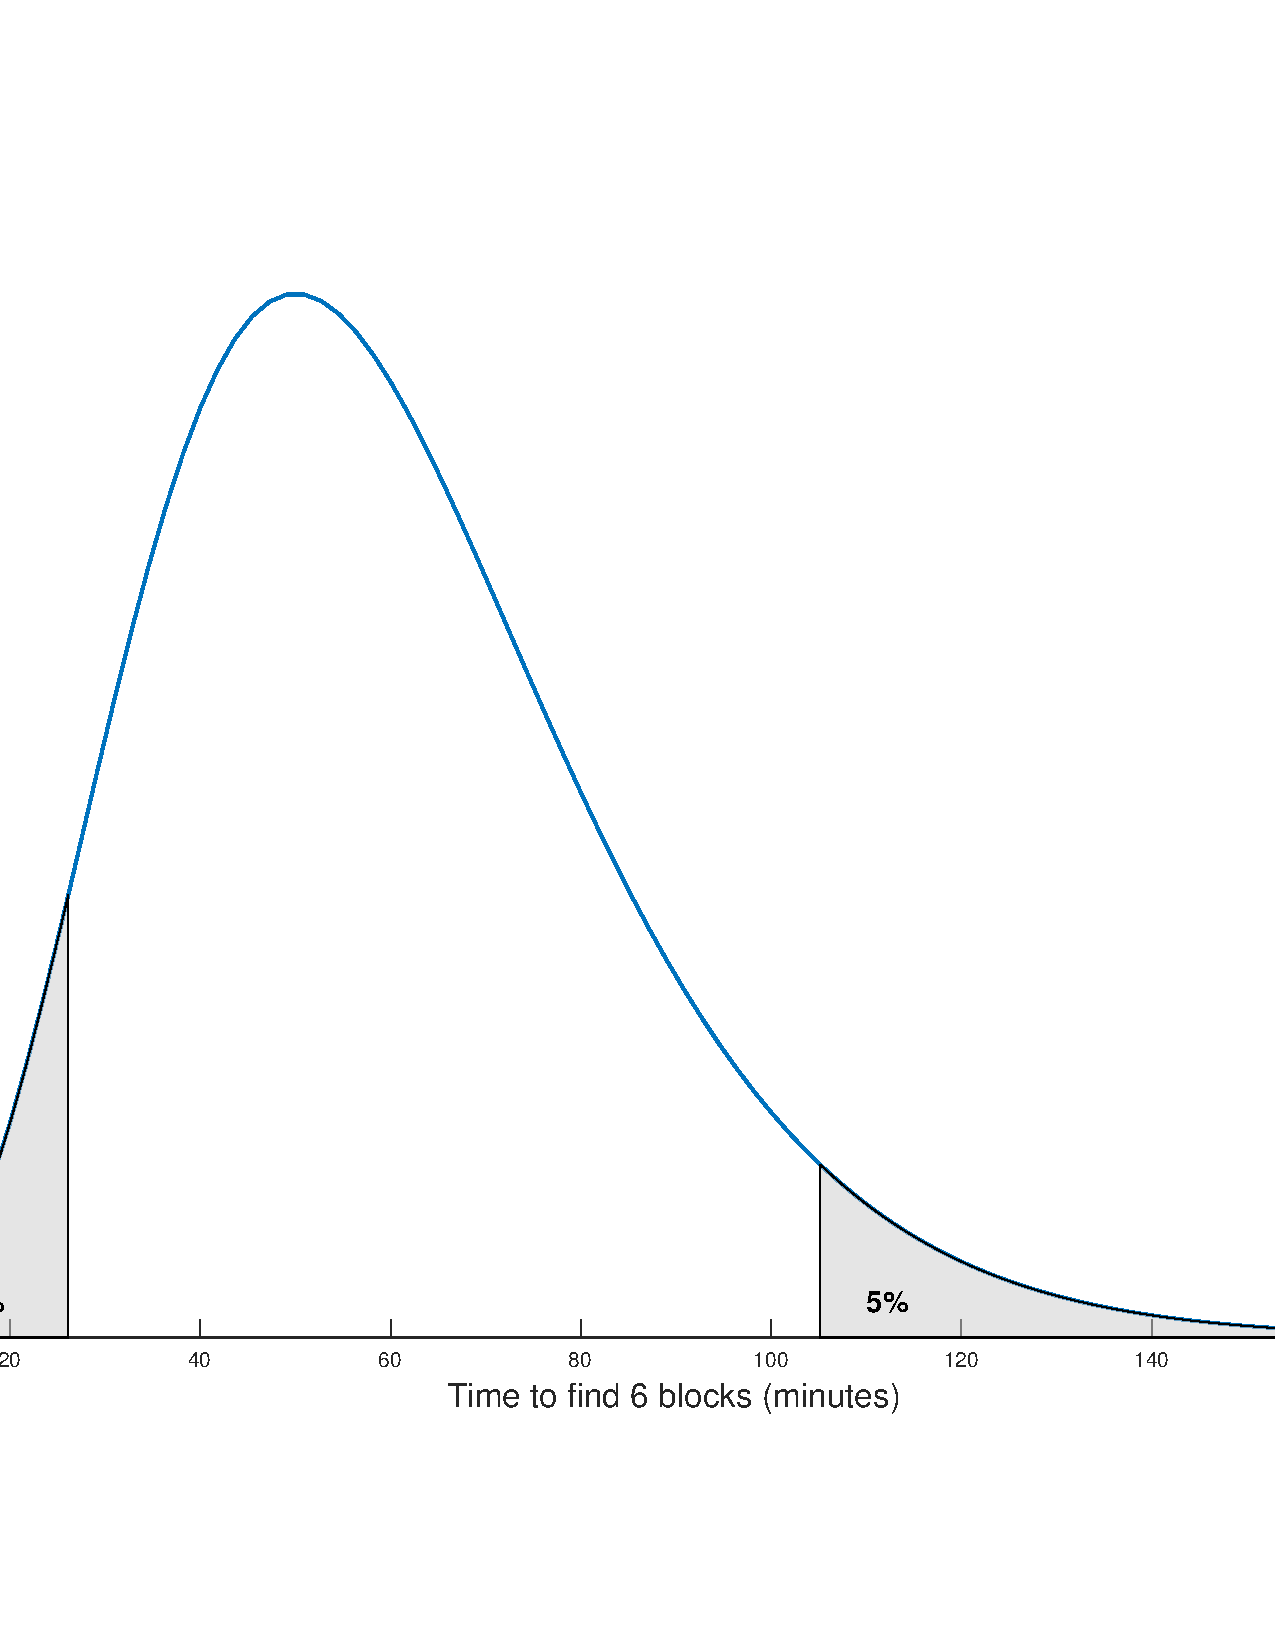
\includegraphics[width=\textwidth]{./images01/time-6-blocks.pdf}
\caption{Probability density function of $Y_6$, i.e., probability of finding 6 blocks after time $t$. The shaded areas shows the lower 5\% and upper 5\% of the pdf.\label{fig-bitcoin-time-6-blocks}}
\end{figure}

\section{Mining for a miner}

Let's analyze the probability of finding a new block for a miner who has $\alpha$ percent of the network's total hash rate. Let $T_\alpha = \frac{X}{\alpha H}$ be the time required for the miner to find a new block. As $T_\alpha = \left( \frac{1}{\alpha} \right) T$, when $H \rightarrow +\infty$, $T_\alpha$ also follows an exponential with parameter $\lambda_\alpha = \frac{\alpha}{\eta}$. Hence, we confirm the intuition that the miner with $\alpha$ percent of the network's total hash power will find $\alpha$ percent of the blocks.

\begin{theorem}
	When the miner with $\alpha$ percent of the network's total hash rate is part of the mining network, $\mathbf{P}(\text{next block is from $T_\alpha$}) = \alpha.$
\end{theorem}
\begin{proof}
\begin{align*}
	\mathbf{P}(\text{next block is from $T_\alpha$}) &= P \left( T_\alpha = \min\{T_\alpha, T_{1-\alpha}\} \right) \\
		&= \frac{\lambda_\alpha}{\lambda_\alpha + \lambda_{1-\alpha}} \\
		&= \frac{\alpha/\eta}{\alpha/\eta + (1-\alpha)/\eta} \\
		&= \frac{\alpha}{\alpha + 1 - \alpha} \\
		&= \alpha.
\end{align*}
\end{proof}

\begin{theorem}
	When one miner with $\alpha$ percent of the network's total hash rate multiplies their hash rate by $m$, the probability of this miner find the next block is multiplied by $\frac{m}{m \alpha + 1 - \alpha}$.
	\label{thm-miner-multiply}
\end{theorem}
\begin{proof}
	When miners increase their hash rate, they also increase the network's total hash rate. Let $H$ be the network's hash rate before the increase. Thus, the network's total hash rate after the increase is $H + (m-1) \alpha H = (1 - \alpha + m \alpha) H$. So,
\begin{align*}
	\mathbf{P}(\text{next block is from $T_{m \alpha}$}) &= P \left( T_{m \alpha} = \min\{T_{m \alpha}, T_{1-\alpha}\} \right) \\
		&= \frac{\lambda_{m \alpha}}{\lambda_{m \alpha} + \lambda_{1-\alpha}} \\
		&= \frac{m \alpha/\eta}{m \alpha/\eta + (1-\alpha)/\eta} \\
		&= \frac{m \alpha}{m \alpha + 1-\alpha} \\
		&= \alpha \left( \frac{m}{m \alpha + 1 - \alpha} \right).
\end{align*}
\end{proof}

\begin{cor}
	If one miner has a really tiny percent of the network's total hash rate, then multiplying their hash rate by $m$ approximately multiplies their probability of finding the next block by $m$.
\end{cor}
\begin{proof}
	$$\lim_{\alpha \rightarrow 0} \mathbf{P}(\text{next block is from $T_{m \alpha}$}) = \lim_{\alpha \rightarrow 0} \frac{m}{m \alpha + 1 - \alpha} = m.$$
\end{proof}

That way, it is not exactly correct to say that when one doubles their hash rate, their probability will double as well. It is only true for small miners.


\section{Orphan blocks}
% Probabilidade de orfão
An orphan block would be created if a new block is found during the propagation time of a new block. Let $\alpha$ be the percentage of the total hash rate of the node which is outdated, and $\Delta t$ the propagation time in seconds. Thus, $\mathbf{P}(\text{new orphan}) = \mathbf{P}(T < \Delta t) = 1 - e^{-\frac{\alpha \Delta t}{\eta}}$.

Bitcoin peer-to-peer network is a gossip network, where miners are semi-randomly connected to each other, and each miner sends all information it receives to all its peers. According to \citet{decker2013information}, the average time for a new block propagate over the network is 12.6 seconds, while the 95\% percentile is 40 seconds, which indicates a long-tail distribution. \citet{bitcoinstats} has measured the propagation time between 2013 and 2017. During 2017, the worst daily 90\% percentile was 21 seconds. Notice that both results may not be contradictory because Bitcoin network is continuously evolving.

For instance, if a node has 10\% of the total hash rate and it takes 30 seconds to receive the update, then $\mathbf{P}(\text{new orphan}) = 1 - e^{-\frac{0.1 \cdot 30}{600}} = 0.004987$, which is almost 0.5\%. I would say that a node with 10\% of the total hash rate would be well connected and it would take less time to receive the update, so, the probability would be even smaller than 0.5\%.

Another important factor is that, as Bitcoin is open-source, miners are free to change the gossip algorithm, which leads to the network incentives. See \citet{babaioff2012bitcoin} for an analysis of the incentives to miners forward new blocks and transactions in the network.

For further information about gossip algorithms, see \citet{shah2009gossip}.


\section{Analysis of network's hash rate change}
% Análise: Mudança no network's hash rate antes de atualizar o $A$.

The difficulty, given by the number $A$, is adjusted every 2016 blocks. As, $\mathbf{P}(13 \text{ days} < Y_{2016} < 15 \text{ days}) = \mathbf{P}(13 \cdot 24 \cdot 3600 < Y_{2016} < 14 \cdot 24 \cdot 3600) = 0.9986$, it is expected that the total time to find 2016 blocks will be between 13 and 15 days, assuming that the network's hash rate remains constant. If it takes less than the expected time, it means that the network's total hash rate has increased. While if it takes more than the expected time, it means that the network's total hash rate has decreased. So, let's analyze what happens when the network's hash rate changes significantly.

%Let's assume that the network's total hash rate will change only once, from $H$ to $\alpha H$ --- so, if $\alpha = 1$, there would be no change, if $\alpha > 1$, there would be an increase, and if $\alpha < 1$, there would be a decrease. As the time required to find a new block would be $T_\alpha = \frac{X}{\alpha H}$, we got the same random variable as we have gotten when analyzing a miner with $\alpha$ percent of the network's total hash rate. But, the analysis will be different because here $\alpha$ may be greater than one.

Let $H \cdot u(t)$ be the network's total hash rate over time. So, the number of hashes calculated in $t$ seconds is $H \int_0^t u(t) dt$. Hence, $\mathbf{P}(T \leq t) = \mathbf{P}(X \leq H \int_0^t u(t)dt)$. When $H \rightarrow +\infty$, $\mathbf{P}(T \leq t) = 1 - e^{-\frac{1}{\eta} \int_0^t u(t) dt}$, and the pdf of $T$ is $\frac{u(t)}{\eta} \cdot e^{-\frac{1}{\eta} \int_0^t u(t)dt}$.

Let's say that the network's total hash rate has suddenly multiplied by $\alpha$. So, $u(t) = \alpha$, $\int_0^t u(t) dt = \alpha t$, and $T$ also follows an exponential distribution, but with $\lambda = \frac{\alpha}{\eta}$. Thus, $Y_n^\alpha = \sum_{i=1}^{n} T_i^\alpha \sim \text{Erlang}(n, \frac{\alpha}{\eta})$. Thus, $\mathbf{E}[Y_{n}^\alpha] = \frac{\mathbf{E}[Y_{n}]}{\alpha}$, i.e., the average total time required to find $n$ blocks will be divided by $\alpha$, while $\mathbf{V}[Y_{n}^\alpha] = \frac{\mathbf{V}[Y_n]}{\alpha^2}$ and the variance will be divided by $\alpha^2$. Hence, on one hand, when the network's hash rate increases ($\alpha > 1$), the 2016 blocks will be found earlier. On the other hand, when the network's hash rate decreases ($\alpha < 1$), the 2016 blocks will be found later.

For example, if the network's total hash rate suddenly doubles ($\alpha = 2$), then $\mathbf{P}(6.5 \text{ days} < Y_{2016} < 7.5 \text{ days}) = 0.9986$, and the time required to find 2016 blocks halved. On the other side, if the network's total hash rate suddenly halves ($\alpha = 0.5$), then $\mathbf{P}(27 \text{ days} < Y_{2016} < 29 \text{ days}) = 0.9469$, and the time required to find 2016 blocks doubled. It is an important conclusion, since it shows that even if half of the network stops mining, it will only double the time to the next difficulty adjustment, i.e., the time between blocks will be 20 minutes for, at most, the next 29 days, at which point the adjustment will occur and everything will be back to the normal 10 minutes between blocks.

% TODO Step-wise analysis

\subsection{Hash rate smoothly changing}

Let $u(t) = \frac{1+abx}{1+bx}$. It is an useful function because $u(0) = 1$ and $\lim_{t \rightarrow \infty} u(t) = a$. The bigger the $b$, the faster $u(t) \rightarrow a$. For example, if $a=2$, it means $H$ would be smoothly doubling. If $a=0.5$, it means $H$ would be smoothly halving.

It is easy to integrate $u(t)$ because $\frac{1+abx}{1+bx} = \frac{1-a}{1+bx} + a \Rightarrow \int_0^t u(x) dx = at + \frac{1-a}{b} \log(1+bt)$. So,
$$F_T(t) = 1 - (1+bt)^{\frac{\lambda(a-1)}{b}} e^{-\lambda at}.$$
$$f_T(t) = \lambda \left( \frac{1+abt}{1+bt} \right) (1+bt)^{\frac{\lambda(a-1)}{b}} e^{-\lambda at}.$$

Assuming that $n = \frac{\lambda(a-1)}{b}$ is integer, we have:
$$F_T(t) = 1 - (1+bt)^n e^{-\lambda at}$$

Thus,
\begin{align*}
\mathcal{L}\{F_T(t)\} &= \mathcal{L}\{1 - (1+bt)^n e^{-\lambda at}\} \\
	&= \mathcal{L}\{1\} - \mathcal{L}\{(1+bt)^n e^{-\lambda at}\} \tag{$\mathcal{L}$ is a linear operator} \\
	&= \frac{1}{s} - \mathcal{L}\{(1+bt)^n e^{-\lambda at}\} \\
	&= \frac{1}{s} - \sum_{k=0}^n \binom{n}{k} b^k \mathcal{L}\{t^k e^{-\lambda at}\} \\
	&= \frac{1}{s} - \sum_{k=0}^n \binom{n}{k} b^k \frac{k!}{(s+\lambda a)^{k+1}}
\end{align*}

Hence, as $\mathcal{L}\{f_T(t)\} = s \mathcal{L}\{F_T(t)\}$,

$$\mathcal{L}\{f_T(t)\} = 1 - \sum_{k=0}^n \binom{n}{k} \frac{s b^k k!}{(s+\lambda a)^{k+1}}$$

Then,

\begin{align*}
\frac{d}{ds} \mathcal{L}\{f_T(t)\}
	&= - \sum_{k=0}^n \binom{n}{k} b^k k! \frac{d}{ds} \frac{s}{(s+\lambda a)^{k+1}} \\
	&= - \sum_{k=0}^n \binom{n}{k} b^k k! \left[ \frac{1}{(s+a\lambda)^{k+1}} - \frac{s(k+1)}{(s+a \lambda)^{k+1}} \right] \\
\frac{d}{ds} \mathcal{L}\{f_T(t)\}|_{s=0}
	&= - \sum_{k=0}^n \binom{n}{k} b^k k! \frac{1}{(\lambda a)^{k+1}} \\
	&= - \frac{1}{a\lambda} \sum_{k=0}^n \binom{n}{k} k! \left( \frac{b}{\lambda a} \right)^k \\
	&= - \frac{1}{a\lambda} \sum_{k=0}^n \frac{n!}{(n-k)!} \left( \frac{b}{\lambda a} \right)^k \\
	&= - \frac{1}{a\lambda} \left[ n! \sum_{k=0}^n \frac{1}{(n-k)!} \left( \frac{b}{\lambda a} \right)^k \right] \\
	&= - \frac{1}{a\lambda} \left[ n! \sum_{k=0}^n \frac{1}{k!} \left( \frac{b}{\lambda a} \right)^{n-k} \right] \tag{$k \rightarrow n-k$} \\
	&= - \frac{1}{a\lambda} \left[ n! \left(\frac{b}{\lambda a}\right)^n \sum_{k=0}^n \frac{1}{k!} \left( \frac{b}{\lambda a} \right)^{-k} \right] \\
	&= - \frac{1}{a\lambda} \left[ n! \left(\frac{b}{\lambda a}\right)^n \sum_{k=0}^n \frac{1}{k!} \left( \frac{\lambda a}{b} \right)^{k} \right]
\end{align*}

Finally, as $\mathbf{E}[T] = -\mathcal{L}\{f_T(t)\}|_{s=0}$,
$$\mathbf{E}[T] = \frac{1}{\lambda a} \left[ n! \left(\frac{b}{\lambda a}\right)^n \sum_{k=0}^n \frac{1}{k!} \left( \frac{\lambda a}{b} \right)^{k} \right] \text{, where $n = \frac{\lambda(a-1)}{b}$}$$

Let's check this equation for already known scenarios. When $a=1$, then $n=0$ and $\mathbf{E}[T] = 1/\lambda$. When $b \rightarrow +\infty$, it reduces to the case in which the hash rate is multiplied by $a$, which we have already studied. In fact, $n \rightarrow 0$, $u(t) \rightarrow a$, and $\mathbf{E}[T] = \frac{1}{\lambda a}$.

\begin{theorem}
	$$a > 1 \text{ and } x > M \Rightarrow \left| \frac{1+abx}{1+bx} - a \right| < \frac{a-1}{1+bM}$$
\end{theorem}
\begin{proof}
$x > M \Rightarrow \frac{1}{1+bx} < \frac{1}{1+bM}$. As $1-a<0$, $\frac{1-a}{1+bx} > \frac{1-a}{1+bM}$. Thus, $\frac{1-a}{1+bM} < \frac{1-a}{1+bx} + a - a = \frac{1+abx}{1+bx} - a < 0 < \frac{a-1}{1+bM}$. Hence, $-\frac{a-1}{1+bM} < \frac{1+abx}{1+bx} - a < \frac{a-1}{1+bM}$.
\end{proof}

For instance, if we would like to know the impact of smoothly double the hash rate in the next week, then the parameters would be $\lambda = 1/600$, $a=2$, $M=1\text{ week}=3600\cdot24\cdot7 = 604,800$, $b$ can be calculated using $\epsilon = \frac{a-1}{1+bM} < 0.01 \Leftarrow b > 0.000163690 \Leftarrow n < 10.1818$. So, for $n=10$, then $b=0.000166666$ and $\epsilon = 0.009823 < 0.01$, as expected. Finally, $\mathbf{E}[T] = 557.65$. In other words, during the next week, the average time between blocks will be 9 minutes and 17 seconds, instead of the normal 10 minutes. If the hash rate had suddenly doubled, the average time between blocks would be 5 minutes.

%$$\mathbf{E}[T] = -\mathcal{L}\{f_T(t)\}|_{s=0} = \frac{b^n n! 600^{n+1}}{a^{n+1}} e^{\frac{a}{600b}} \text{, where $n = \frac{a-1}{600b}$}$$


%$a > 1, x > M \Rightarrow 1 + bx > 1 + bM \Rightarrow \frac{1}{1+bx} < \frac{1}{1+bM} \Rightarrow \frac{1-a}{1+bx} + a > \frac{1-a}{1+bM} + a \Rightarrow \frac{1+abx}{1+bx} - a > \frac{1-a}{1+bM}$.


\subsection{Piecewise linear model of hash rate change}

Let's analyze what would happen if the network's hash rate is growing linearly with angular coefficient $a^2$, i.e., $u(a, b, t) = a^2t + b$. Thus, $\mathbf{P}(T \leq t) = 1 - e^{-\frac{bt + a^2t^2/2}{\eta}}$.

It is well known that $\mathbf{E}(T) = \int_{0}^{\infty} 1 - \mathbf{P}(T \leq t) dt$. Thus, replacing $y = \frac{a^2 t + b}{a \sqrt{2 \eta}}$, and using the fact that $\int_0^\infty e^{-x^2} dx = \frac{\sqrt{\pi}}{2} \erf(x)$, we have:

\begin{align}
\mathbf{E}(T)|_{t_1}^{t_2} &= \int_{t_1}^{t_2} \exp \left( - \frac{bt + a^2 t^2/2}{\eta} \right) dt \nonumber \\
	&= \frac{\sqrt{2 \eta}}{a} \exp \left( \frac{b^2}{2a^2 \eta} \right) \int_{y_1}^{y_2}  \exp(-y^2) dy \nonumber \\
	&= \frac{\sqrt{2 \eta}}{a} \exp \left( \frac{b^2}{2a^2 \eta} \right) \frac{\sqrt{\pi}}{2} [\erf(y_1) - \erf(y_2)] \nonumber \\
	&= \frac{\sqrt{2 \pi \eta}}{2a} \exp \left( \frac{b^2}{2a^2 \eta} \right) \left[\erf(y_2) - \erf(y_1) \right]
\end{align}

Where $y_1 = \frac{a^2 t_1 + b}{a \sqrt{2 \eta}}$ and $y_2 = \frac{a^2 t_2 + b}{a \sqrt{2 \eta}}$.

Thus, $\mathbf{E}(T) = \mathbf{E}(T)|_0^\infty$. When $t_1 = 0 \Rightarrow y_1 = \frac{b^2}{2 \sqrt{2 \eta}}$ and $t_2 \rightarrow \infty \Rightarrow y_2 \rightarrow \infty \Rightarrow \erf(y_2) = 1$, then:

$$
\mathbf{E}(T) = \frac{\sqrt{2 \pi \eta}}{2a} \exp \left( \frac{b^2}{2a^2 \eta} \right) \left[1 - \erf\left(\frac{1}{a \sqrt{2 \eta}}\right)\right]
$$

The function $\mathbf{E}(T)|_{t_1}^{t_2}$ may be used to a piecewise linear analysis of any hash rate change. Let's analyze the hash doubling in one week. Then, $u(1 \text{week}) = u(604800) = 2$, thus $a^2 = \frac{1}{604800} \Rightarrow a = \frac{1}{120 \sqrt{42}}$. Let's sample the interval $[0, 1 \text{week}]$ every hour, i.e., ($t_0$, $t_1$, $t_2$, \dots, $t_168$), where $t_i = i \cdot 1 \text{hour} = i \cdot 3600$.

For each point $t_i$, let $g_i(t) = [H(t-t_i) - H(t-604800)] u(t) + 2 H(t-604800)$, then $\mathbf{E}(T) = \mathbf{E}(T)|_{t_i}^{t_{i+1}} + 1 - e^{\frac{t}{\eta}}$. The result is presented in Figure .

%In order to obtain $\mathbf{E}(T)$, we will use the formula $\frac{d}{ds}T^*(s)|_{s=0} = -\mathbf{E}(T)$, where $T^*$ is the Laplace transform of the pdf of T.
%
%Let $f_T(x)$ be the pdf of T and $F_T(x)$ be the cdf of T, i.e., $F_T(x) = \int_0^x f_T(t) dt$. Thus, $\mathcal{L}\{F_T(x)\} = \frac{T^*(s)}{s}$.
%
%\begin{align*}
%	\mathcal{L}\{F_T(x)\} &= \int_0^\infty e^{-sx} F_T(x) dx \\
%		&= \int_0^\infty e^{-sx} \left( 1 - e^{-\frac{x + a^2x^2/2}{\tau}} \right) dx \\
%		&= \int_0^\infty e^{-sx} dx - \int_0^\infty e^{-sx} e^{-\frac{x + a^2x^2/2}{\tau}} dx \\
%		&= \frac{1}{s} - \int_0^\infty e^{-sx -\frac{x + a^2x^2/2}{\tau}} dx \\
%\end{align*}
%
%Let $b=\frac{a}{\sqrt(2 \tau)}$ and $c = \frac{\sqrt(2 \tau)}{2a} \left( s + \frac{1}{\tau} \right)$, then $sx + \frac{x+a^2x^2/2}{\tau} = (bx + c)^2 - c^2$.
%Let $y = bx+c \Rightarrow dy = bdx$.
%
%\begin{align*}
%	\int_0^\infty e^{-sx -\frac{x + a^2x^2/2}{\tau}} dx &= \int_0^\infty e^{-(bx+c)^2 + c^2} dx \\
%		&= \int_c^\infty e^{-y^2 + c^2} \frac{dy}{b} \\
%		&= \frac{e^{c^2}}{b} \int_c^\infty e^{-y^2} dy \\
%		&= \frac{\sqrt{\pi}e^{c^2}}{2b} \erfc(c)
%\end{align*}
%
%$$ \mathcal{L}\{F_T(x)\} = \frac{1}{s} - \frac{\sqrt{\pi}e^{c^2}}{2b} \erfc(c) $$
%
%Hence,
%$$ T^*(s) = s \mathcal{L}\{F_T(x)\} = 1 - \frac{s\sqrt{\pi}e^{c^2}}{2b} \erfc(c) $$
%
%As $\frac{d}{ds}c = \frac{\sqrt{2 \tau}}{2a}$,
%
%\begin{align*}
%\frac{d}{ds} T^*(s) &= - \frac{\sqrt{\pi}e^{c^2}}{2b} \erfc(c) - \frac{\sqrt{2 \tau \pi} sc e^{c^2}}{2ab} \erfc(c) + \frac{\sqrt{2 \tau \pi}s}{4ab} \\
%\frac{d}{ds} T^*(s)|_{s=0} &= - \frac{\sqrt{2 \tau \pi}}{2a} e^{\frac{1}{2 \tau a^2}} \erfc\left(\frac{1}{a \sqrt{2 \tau}}\right) \\
%\mathbf{E}[T] &= \frac{\sqrt{2 \tau \pi}}{2a} e^{\frac{1}{2 \tau a^2}} \erfc\left(\frac{1}{a \sqrt{2 \tau}}\right) \\
%\end{align*}
%
%$\mathbf{E}[T]$ is ploted for $a \in (0, 0.1]$ at Figure \ref{fig-bitcoin-H-increase}. The plot interval is really small because $a=1$ would imply doubling the hash rate after 1 second.
%
%\textcolor{red}{I do not know how to interpret this.}

\begin{figure}[ht]
\centering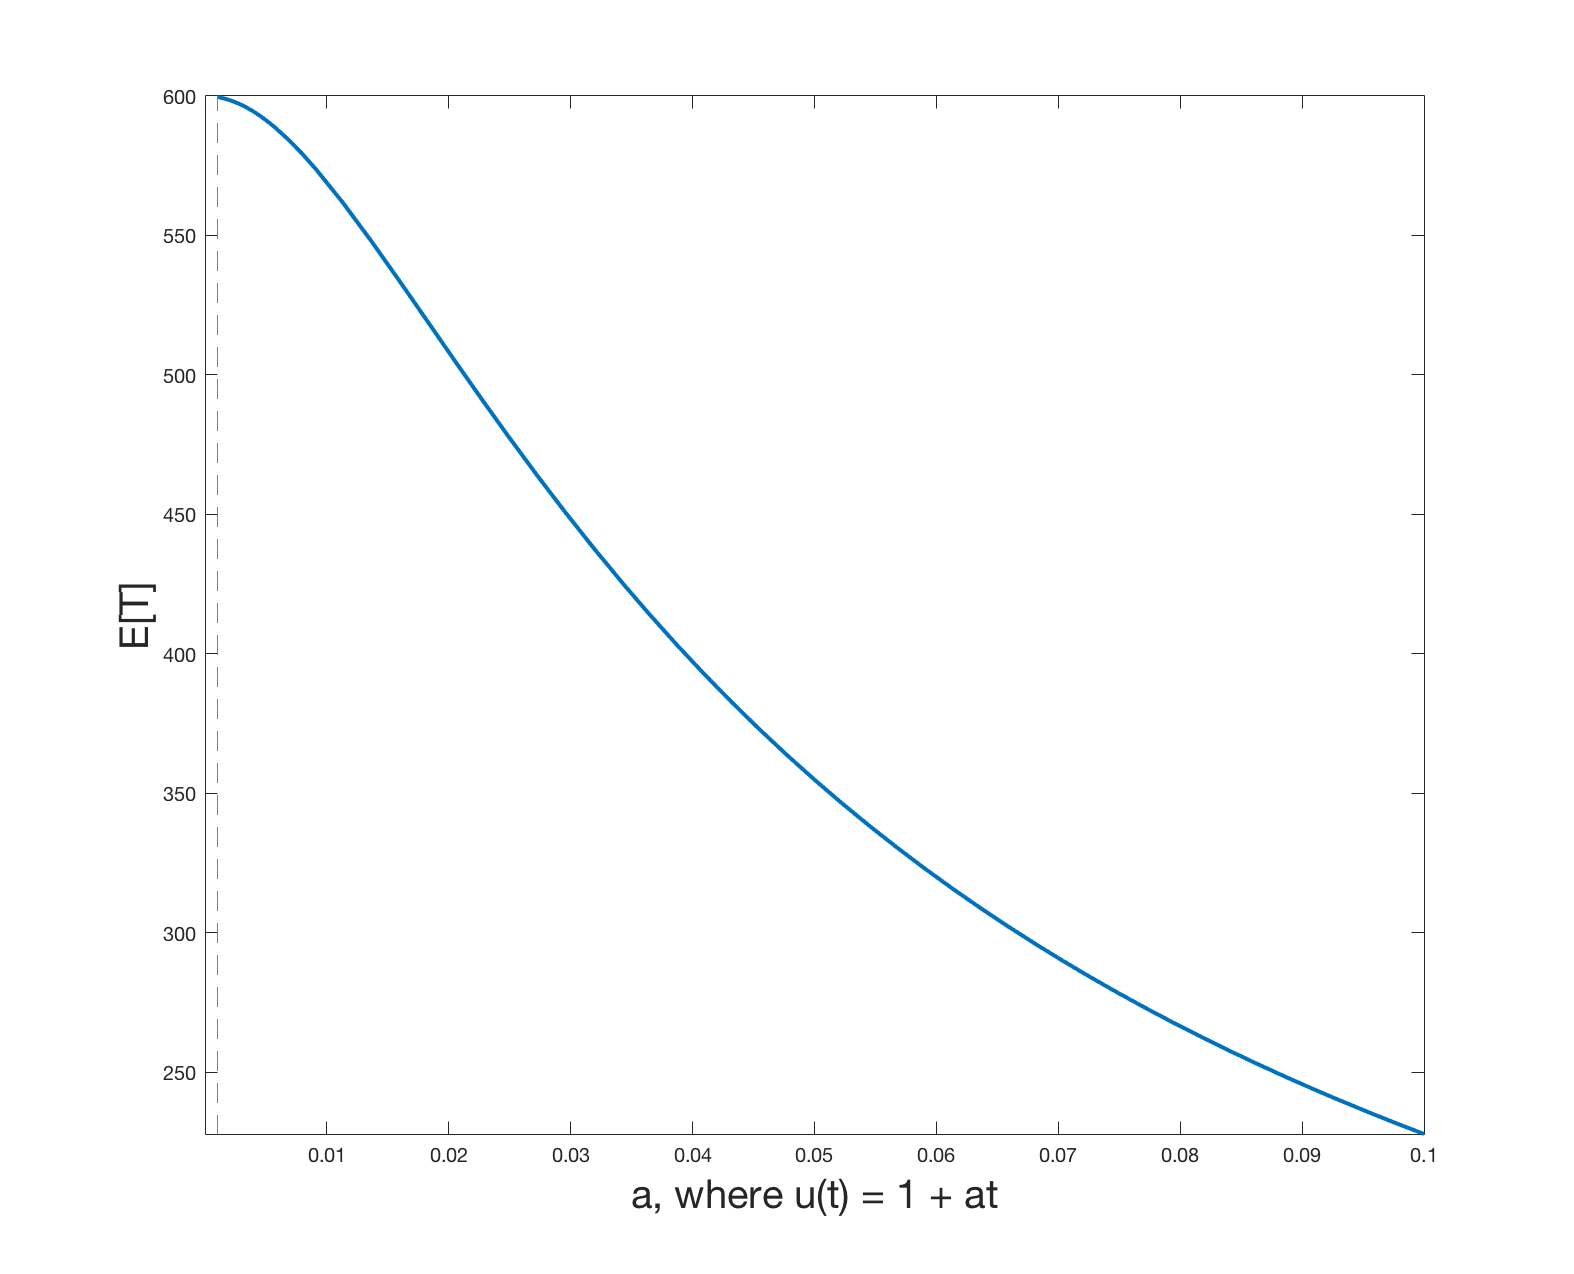
\includegraphics[width=\textwidth]{./images01/bitcoin-H-increasing.png}
\caption{$\mathbf{E}[T]$ when H increases linearly with $u(t) = 1 + at$.\label{fig-bitcoin-H-increase}}
\end{figure}


\section{Attack in the Bitcoin network}
% Ataque submarino
% Probabilidade de "correr por fora"

\citet{karame2012two}

There are many possible ways to attack the Bitcoin (REF). In this section, we are interested in a particular attack: the double spending attack.

In the double spending attack, the attacker's send some funds to the victim, let's say a merchant. They wait for $k$ confirmations of the transaction, and the victim delivers the good or the service to the attacker. Then, the attacker mine enough blocks with a conflicting transaction, double spending the funds which was sent to the victim. If the attacker is successful, the original transaction will be \textit{erased} and the victim will be left with no funds at all. In order to be successful, the attacker must propagate more blocks than the network in the same period, propagating a chain longer than the main chain. Hence, we would like to understand what the odds are that the attacker will be successful. This attack was originally discussed by \citet{nakamoto2008bitcoin}.

In order to maximize their odds, the attacker must start to mine the new blocks as soon as they send the funds to the victim. In this moment, it starts to mine in the head of the blockchain, just like the rest of the network. So, in the beginning, the attacker and the network are in exactly the same point.

Let $\beta H$ be the hash rate of the attackers, and $\gamma H$ be the network's hash rate without the attackers. Thus, when $H \rightarrow +\infty$, we already know that $T_{\text{attackers}}$ and $T_{\text{network}}$ follow exponential distributions with parameters $\lambda_{\text{attacker}} = \frac{\beta}{\eta}$ and $\lambda_{\text{network}} = \frac{\gamma}{\eta}$, respectively.

As \cite{nakamoto2008bitcoin} has done, we will also model the attack using the Gambler's Ruin. In this game, a gambler wins \$1 at each round, with probability $p$, and loses \$1, with probability $1-p$. The rounds are independent. The gambler starts with \$$k$ plays continuously until he either accumulates a target amount of \$$m$, or loses all his money. Let $\rho = \frac{1-p}{p}$, then the probability of losing his fortune is:

$$
\mathbf{P}(\text{losing his fortune}) =
\begin{cases}
	\frac{\rho^k - \rho^m}{1-\rho^m} \text{, if $\rho \ne 1$,} \\
	\frac{m-k}{m} \text{, if $\rho = 1$.}
\end{cases}
$$

When $m \rightarrow +\infty$,

$$
\mathbf{P}(\text{losing his fortune}) =
\begin{cases}
	\rho^k \text{, if $\rho < 1$,} \\
	1 \text{, if $\rho \geq 1$.}
\end{cases}
$$

% TODO Expected time to absorption.

The gambler winning \$1 is the same as the network finding a new block, the gambler losing \$1 is the same as the attacker finding a new block. The initial \$$k$ is the same as the number of blocks the attacker is behind the network. Thus, the gambler loses his fortune is the same as the attacker successfully finds $k$ or more blocks than the network, i.e., losing his fortune means that the attack was successful.

In our case, $p = \frac{\lambda_{\text{network}}}{\lambda_{\text{network}} + \lambda_{\text{attacker}}} = \frac{\gamma}{\beta + \gamma}$, thus $\rho = \frac{\beta}{\gamma}$. Hence, $\rho < 1 \Leftrightarrow \beta < \gamma$.

Suppose that the attacker is mining with the network. Suddently, he stops mining with the network and starts attacking, i.e., starts to mine in another chain. In this scenario, since the attacker's hash rate is not mining with the network anymore, $\gamma = 1 - \beta$. Thus, $\beta < \gamma \Rightarrow \beta < 0.5 \Leftrightarrow \rho < 1$. Here comes the conclusion that, if the attacker has 50\% or more of the network's hash rate, then his attack will be certainly successful. We got exactly the same equations and conclusions as \cite{nakamoto2008bitcoin}.

But this scenario seems not to be the optimal attack, because the attacker has waited $k$ confirmations before starting the attack. A better approach would be to start attacking just after propagating the transaction. In this case, our previous model is not good, because even if the attacker have found more blocks than the network, he cannot propagate those blocks before the network has found $k$ confirmations. So, we have to model the probabilities before the network has found the $k$ block. Then, if the attacker has more blocks than the network, he has successfully attacked. Otherwise, we return to the previous model, in which the attacker must still find more blocks.

\begin{theorem}
	Assuming that the attacker starts the attack just after publishing the transaction, the probability of the attacker has already found exactly $s$ blocks while it waits the network to find $k$ blocks is $\mathbf{P}(S = s) = \binom{k+s-1}{s} (1-p)^s p^k.$
\end{theorem}
\begin{proof}
The attacker must find exactly $s$ blocks while the network must find exactly $k$ blocks. It is as they would be walking the grid from the point $(0, 0)$ to $(s, k)$, where it is only allowed to go up or right, like in Figure \ref{figure:bitcoin-attack-paths}. When the attacker finds a block, it would be a movement to the right. When the network finds a block, it would be an upward movement. No matter the order which the blocks are found, all the paths occur with probability $(1-p)^s p^k$.

The walking ends when $(\cdot, k$) is reached, i.e., when the network finds $k$ blocks, regardless of how many blocks the attacker has found -- i.e., it is not allowed to walk above the line $(\cdot, k)$. Thus, the number of paths between $(0, 0)$ and $(s, k)$ moving only upward or to the right, without going into the line $(\cdot, k)$ is exactly the number of paths between $(0, 0)$ and $(s, k-1)$, which is equal to the number of permutations of the sequence $(u, u, \dots, u, r, r, \dots, r)$ in which there are $s$ movements to the right ($r$) and $k-1$ upward movements ($u$). This number of permutations is $\frac{(k-1+s)!}{s!(k-1)!} = \binom{(k-1)+(s)}{s}$ because there are $s$ repetitions of the element $r$ and $k-1$ repetitions of the element $u$.

Finally, the probability is $\binom{k+s-1}{s} (1-p)^{s} p^{k}$.

\begin{figure}[ht]
  \centering
  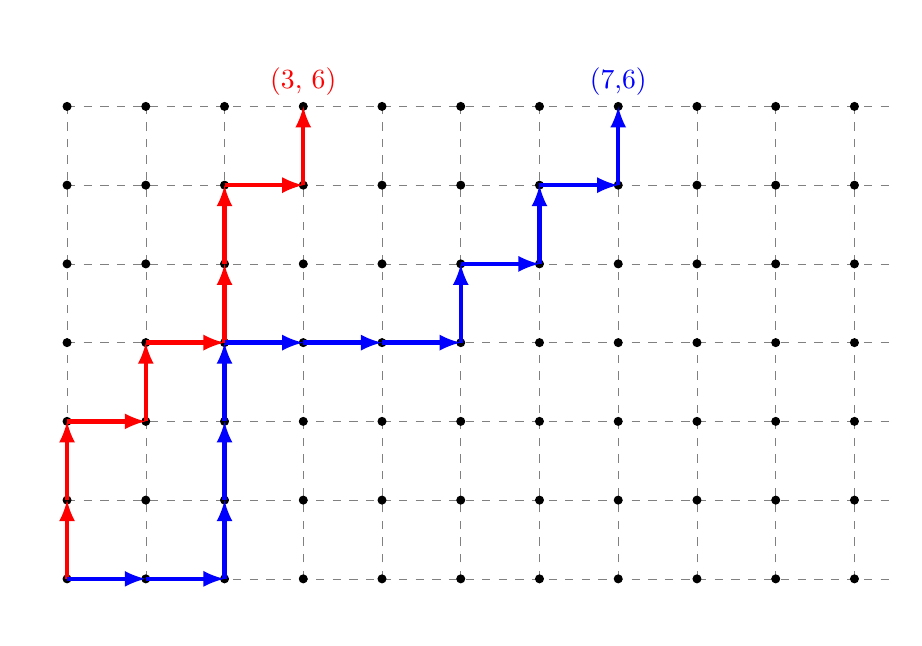
\begin{tikzpicture}
    \coordinate (Origin)   at (0,0);
    \coordinate (XAxisMin) at (-1,0);
    \coordinate (XAxisMax) at (5,0);
    \coordinate (YAxisMin) at (0,-1);
    \coordinate (YAxisMax) at (0,5);
    %\draw [thin, gray,-latex] (XAxisMin) -- (XAxisMax);% Draw x axis
    %\draw [thin, gray,-latex] (YAxisMin) -- (YAxisMax);% Draw y axis

    \clip (-0.5,-0.5) rectangle (10.5cm,7cm); % Clips the picture...
    %\pgftransformcm{1}{0}{0}{1}{\pgfpoint{0cm}{0cm}}
          % This is actually the transformation matrix entries that
          % gives the slanted unit vectors. You might check it on
           % MATLAB etc. . I got it by guessing.
    \draw[style=help lines,dashed] (0,0) grid[step=1cm] (14,6);
          % Draws a grid in the new coordinates.
          %\filldraw[fill=gray, fill opacity=0.3, draw=black] (0,0) rectangle (2,2);
              % Puts the shaded rectangle
    \foreach \x in {0,1,...,10}{% Two indices running over each
      \foreach \y in {0,1,...,6}{% node on the grid we have drawn
        \node[draw,circle,inner sep=1pt,fill] at (\x,\y) {};
            % Places a dot at those points
      }
    }

    \draw [ultra thick,-latex,red] (0,0) -- (0,1) node [midway, left] {};
    \draw [ultra thick,-latex,red] (0,1) -- (0,2) node [midway, left] {};
    \draw [ultra thick,-latex,red] (0,2) -- (1,2) node [midway, above] {};
    \draw [ultra thick,-latex,red] (1,2) -- (1,3) node [midway, right] {};
    \draw [ultra thick,-latex,red] (1,3) -- (2,3) node [midway, right] {};
    \draw [ultra thick,-latex,red] (2,3) -- (2,4) node [midway, right] {};
    \draw [ultra thick,-latex,red] (2,4) -- (2,5) node [midway, right] {};
    \draw [ultra thick,-latex,red] (2,5) -- (3,5) node [midway, right] {};
	\draw [ultra thick,-latex,red] (3,5) -- (3,6) node [above] {(3, 6)};

    \draw [ultra thick,-latex,blue] (0,0) -- (1,0) node [midway, left] {};
    \draw [ultra thick,-latex,blue] (1,0) -- (2,0) node [midway, left] {};
    \draw [ultra thick,-latex,blue] (2,0) -- (2,1) node [midway, left] {};
    \draw [ultra thick,-latex,blue] (2,1) -- (2,2) node [midway, left] {};
    \draw [ultra thick,-latex,blue] (2,2) -- (2,3) node [midway, left] {};
    \draw [ultra thick,-latex,blue] (2,3) -- (3,3) node [midway, left] {};
    \draw [ultra thick,-latex,blue] (3,3) -- (4,3) node [midway, left] {};
    \draw [ultra thick,-latex,blue] (4,3) -- (5,3) node [midway, left] {};
    \draw [ultra thick,-latex,blue] (5,3) -- (5,4) node [midway, left] {};
    \draw [ultra thick,-latex,blue] (5,4) -- (6,4) node [midway, left] {};
    \draw [ultra thick,-latex,blue] (6,4) -- (6,5) node [midway, left] {};
    \draw [ultra thick,-latex,blue] (6,5) -- (7,5) node [midway, left] {};
	\draw [ultra thick,-latex,blue] (7,5) -- (7,6) node [above] {(7,6)};
  \end{tikzpicture}
  \caption{Both the attacker and the network are mining. Each step up is a new block found by the network with probability $p$. Each step right is a new block found by the attacker with probability $1-p$. It ends when the network finds $k$ blocks --- in this example, $k=6$. The red path has probability $p^6 (1-p)^3$, while the blue path has probability $p^6 (1-p)^7$. Notice that the blue path is a successfull attack, because the attacker has found more blocks than the network. In the red path, the attacker still have to catch up 3 blocks to have a successful attack, which happens with probability $\rho^3$, if $p < 0.5$.}
  \label{figure:bitcoin-attack-paths}
\end{figure}
\end{proof}

Assuming that the attacker starts mining just after publishing the victim's transaction, the probability of the attacker will have found more than $k$ blocks while it waits the network to find $k$ blocks is $\mathbf{P}(S \geq k) = \sum_{s=k}^{\infty} \binom{k+s-1}{s} (1-p)^s p^k$.

\begin{theorem}
	$$\mathbf{P}(S \geq k) = 1 - \sum_{s=0}^{k-1} \binom{k+s-1}{s} (1-p)^s p^k.$$
\end{theorem}
\begin{proof}
	Let's use the following identity:
	$$\frac{1}{(1-z)^{a+1}} = \sum_{i=0}^{\infty} \binom{i+a}{i} z^i \text{, for $|z|<1$}$$

	Thus, replacing $z=1-p$, $i=s$, and $a=k-1$, we have:

	$$\frac{1}{p^{k}} = \sum_{s=0}^{\infty} \binom{s+k-1}{s} (1-p)^s$$
	$$1 = \sum_{s=0}^{\infty} \binom{s+k-1}{s} (1-p)^s p^k.$$

	Now, just split $\sum_{s=0}^{\infty} = \sum_{s=0}^{k-1} + \sum_{s=k}^{\infty}$ and it is done.
\end{proof}

Using this last theorem, we moved from an infinity sum to a finity sum.

\begin{theorem}
	Let $p = \frac{\gamma}{\beta + \gamma}$.
$$
\mathbf{P}(\text{successful attack}) =
\begin{cases}
%1 - \sum_{s=0}^{k-1} \binom{k+s-1}{s} (1-p)^s p^k \left(1 - \left( \frac{1-p}{p} \right)^{k-s} \right)
	1 - \sum_{s=0}^{k-1} \binom{k+s-1}{s} \left( (1-p)^s p^k - (1-p)^k p^s \right) \text{, $p \geq 0.5$} \\
	1 \text{, $p < 0.5$}.\\
\end{cases}
$$
\end{theorem}
\begin{proof}
$$
\mathbf{P}(\text{successful attack}) = \mathbf{P}(S \geq k) + \sum_{i=0}^{k-1} \mathbf{P}(s=i) \rho^{k-i}
$$
\end{proof}


For $k=6$, $p=0.9$, $\mathbf{P}(\text{successful attack}) = 0.0005914121600000266$.

For $k=6$, $p=0.7$, $\mathbf{P}(\text{successful attack}) = 0.15644958192000014$.

\begin{figure}[ht]
\centering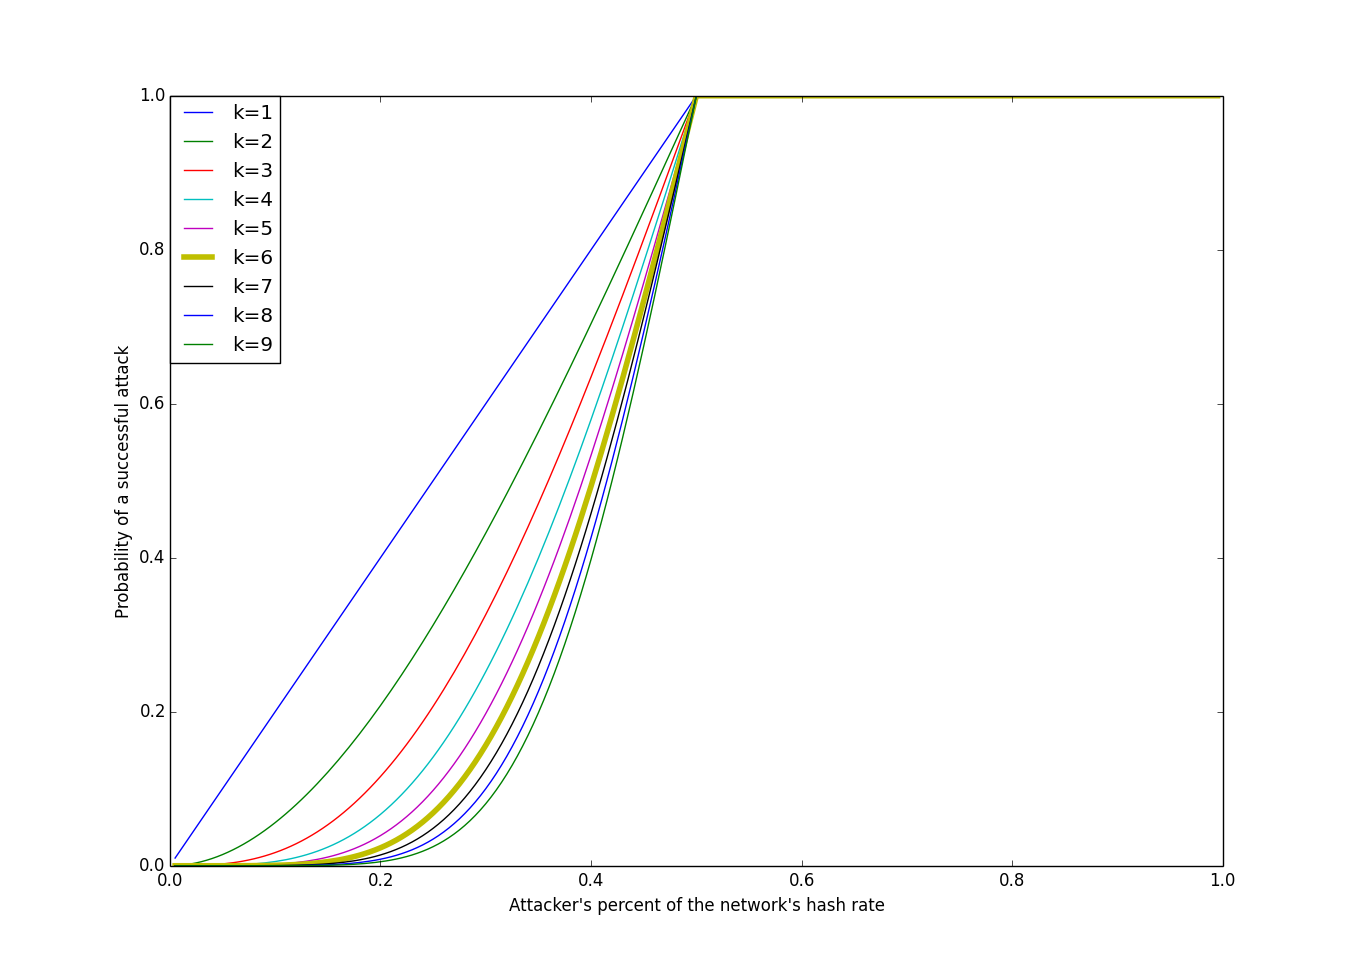
\includegraphics[width=\textwidth]{./images01/fig-bitcoin-attack.png}
\caption{Probability of a successful attack according to the network's hash rate of the attacker ($\beta$).\label{fig-bitcoin-attack}}
\end{figure}

%The number of blocks found in a given time interval $\Delta t$ is given by the Poisson distribution. So, the number of blocks found by the attackers $N_{\text{attacker}}$ follows a Poisson distribution with parameter $\lambda_{\text{attacker}} \Delta t = \frac{\beta \Delta t}{600}$, and the number of blocks found by the network $N_{\text{network}}$ follows a Poission distribution with parameter $\lambda_{\text{network}} \Delta t = \frac{\gamma \Delta t}{600}$. We would like to calculate $\mathbf{P}(N_{\text{attackers}} - N_{\text{network}} \geq k)$.

%$\mathbf{P}(Y_{n+k}^{\text{attacker}} < Y_{n}^{\text{network}})$


\section{Confirmation time and network capacity}
% Tempo na fila para confirmar transação

Let's say that when a new transaction is propagated it is enqueued in the unconfirmed transaction queue. Then, when a new block is found, some of these transactions in the queue are confirmed. We are interested in some measures of the queue, like the expected time to confirm a transaction and the queue's length.

Let's assume that all transactions have exactly the same size $S$ and pay exactly the same fee. If the Bitcoin block's maximum size is $M$, there would be room for $s = \lfloor M/S \rfloor$ transactions in each block. Using the results from \citet{bailey1954queueing}, we have found that $\pi_n = \frac{z_s-1}{z_s^{n+1}}$ is the probability of having $n$ unconfirmed transactions in the pool subjected to $s > m$, where $m=\frac{\lambda_{\text{TX}}}{\lambda_{\text{blocks}}}$ and $z_s$ is the single root of the polynomial $z^s(1+m(1-z))-1$ with $|z_s|>1$. The average size of the unconfirmed transaction pool is $\mathbf{E}(\pi) = \frac{1}{z_s - 1}$. Thus, $s > m \Rightarrow \lambda_{\text{TX}} < s \lambda_{\text{blocks}}$. The probabilities form a simple geometric series, and so they are exponentially decreasing. We may interpret it as a stable system, i.e., the unconfirmed transactions pool size is finite. In the Bitcoin's network, $\lambda_{\text{blocks}} = 1/\eta$ and the average number of transactions per block is $s=2,250$, so, this solution is valid when $\lambda_{\text{TX}} < 2,250/600 = 3.75$. Hence, $3.75$ is the maximum number of new transactions per second that the Bitcoin's network may handle. When $\lambda_{\text{TX}} > 3.75$, the unconfirmed transaction pool starts to grow indefinitely.

The average waiting time of a transaction to be confirmed, when $m < s$, is $\mathbf{E}(w) = \frac{1}{\lambda_{\text{TX}} (z_s-1)}$.

When $m \ll s$, $z_s \rightarrow 1 + 1/m$. So, the average number of unconfirmed transactions is $\mathbf{E}(\pi) \rightarrow m$ and the average waiting time $\mathbf{E}(w) \rightarrow \frac{1}{\lambda_{\text{blocks}}} = \eta = 600 \text{ seconds}$. In the Bitcoin's network, $s \gg m \Rightarrow \lambda_{\text{TX}} \ll 3.75$.

When $\lambda_{\text{TX}} \rightarrow s$, $z_s \rightarrow 1$. So, $\mathbf{E}(\pi) \rightarrow +\infty$.

Finally, we conclude that the Bitcoin's network capacity is $\lambda_{\text{blocks}} s = s/\eta = s/600$ transactions per second, where $s$ is the average number of transactions per block.


\section{Fork analysis}

% TODO BIP's and signaling bit --- see BIP 9 and BIP 135.

When a disagreement between miners' rules happens, that is referred as either a hard-fork or a soft-fork. It is said to be a soft-fork when the rules are backward compatible, and a hard-fork when the rules are not backward compatible. In general, a hard-fork relaxes the constraints, while the latter hardens them.

Suppose that the miners' are split in two groups, $G_1$ and $G_2$, with different rules. Let's say $H_1$ and $H_2$ are their hash rate, respectively. We have two different scenarios to analyze: (i) when neither of them accepts other's blocks; and (ii) when $G_2$ accepts $G_1$'s blocks, but not the other way around.

Scenario (i) is easy to analyze, because the network would just split and, after a while, both difficulties will be adjusted. Then, they will be just like two different Bitcoin networks.

Scenario (ii) is more trick. As $G_2$ accepts $G_1$ blocks, their hashrate will matter. If $H_1 > H_2$, then $G_2$ will frequently skip their blockchain, because $G_1$'s blockchain will be longer most of the time. If $H_1 < H_2$, then $G_2$ may have its own blockchain after a while --- a true fork. But what would happen if $H_1$ keeps increasing and eventually gets larger than $H_2$? It if happens for sufficient time, the whole $G_2$'s blockchain may be discarded in order to move to $G_1$'s blockchain when $G_1$'s gets longer.

\begin{theorem}
	When $H_1 > H_2$, the
\end{theorem}



%What would happen if, after a while, the groups agree again. How would the blockchain merge?


\chapter{Iota \& Tangle}

Iota's underlying technology is Tangle, which has DAG-based architecture with a whole different approach to confirmations. It proposes that there is no need for a block to confirm transactions, as transactions can confirm themselves. Here, each transaction has its own proof-of-work, named weight, and they must confirm two other previous transactions. In this sense, instead of a chain of blocks, the transactions and their confirmations form a directed and acyclic graph (DAG), as in Fig. \ref{fig-tangle-example}.

Like Blockchain, Tangle is another technology to store immutable data and may be the underlying technology to different applications, such as cryptocurrencies, digital contracts (Ethereum-like), digital notaries, and so forth.

Transactions may be either confirmed or unconfirmed. The confirmed transactions have been already confirmed by at least one more transaction. It does not mean they are already irreversible and protected against a double spend attack --- it just means at least one transaction has done some work to confirm it. The unconfirmed transactions are called tips and they are eager to be confirmed. Usually a new transaction selects two tips to confirm, but this rule may not be followed.

Different from Bitcoin, transactions does not have scripts to check whether one may spend the tokens. Instead, it uses a fixed Winternitz hash-based digital signature \citep{dods2005hash}, i.e., whoever correctly signs the transaction may tranfer the tokens. It also supports multi-signature scheme (see \cite{iotamultisign}). Not allowing scripts is a disadvantage when compared to Bitcoin because future applications are limited and changing it would require a major modification in transaction format.

At the beginning, the digital signature algorithm relied on the Curl hash function, which is a ternary hash function designed by Iota's developers. This hash function was replaced by the Kerl hash function after \cite{heilman2017iota} has found a critical vulnerability which enabled practical signature forgery attacks. The Kerl hash function is a variation of SHA-3 also designed by Iota's developers \citep{iotakerl}. Like the Curl hash function, Kerl has not been deeply studied by cryptography researchers and may have critical vulnerabilities.

Iota's tokens are pre-mined, which means they have been issued in the genesis transaction and no more tokens will ever be issued. This means there are no miners in Iota's network and only the users keep the network alive through their new transactions. If, for any reason, the number of transactions per second plummet, the time to confirmed the most recent transactions will increase significantly. This possibly poses a serious risk to the network stability and users' trustworthy.

As there are no miners, there are also no fees, which is a major incentive to new comers. Tokens may be freely transfered without any loses, even for tiny amounts, enabling micropayments. For example, online workers paid per hour may receive their payments every hour, reducing the default risk. This allows untrusted parties to work together reducing the risk for both. The contractor always wants to pay in the end, while the workers always wants to get paid in the beginning.

Not having fees is also also an important feature to the Internet-Of-Things (IoT) technologies. The IoT is a network of smart devices that are connected to the internet and exchange data. It allows, for instance, your refrigerator to do your groceries and automatically pay using your Iota tokens. It also allows your electric car to automatically pay for recharge. For further information, see \cite{fleisch2010internet}.

Theoretically, Iota's network benefits from high volume of transactions. The more transactions are coming, the faster previous transactions are confirmed. This is a major feature of Tangle which contrasts with Bitcoin's difficulty to scale. On the other hand, low volume of transactions is a primary problem for Iota, since it would take too long to confirm previous transactions. As it is a known problem, Iota has created a central coordinator which works as a trustworthy node, clearing transactions. In other words, every transaction directly or indirectly confirmed by the central coordinator is assumed to be cleared. Iota's developers claims that the coordinator will be turned off when the network outgrows a minimum (unknown) size.

An important factor of Iota is how the new transactions choose which transactions they will confirm. There are several possible approaches, such as randomly selecting two of the unconfirmed transactions (tips). In Fig \ref{fig-tangle-example}, the reader may have noticed that transaction 8 will confirm transaction 4, which has already been confirmed by transaction 7. It may be on purpose, or maybe transaction 4 was unconfirmed when it was chosen, but it got confirmed during the calculation of the proof-of-work or the network propagation of the transaction. The selection algorithm seems to be important to protect the network against double spend attacks. For further information, see \cite{tangle2016}.

\begin{figure}[ht]
\centering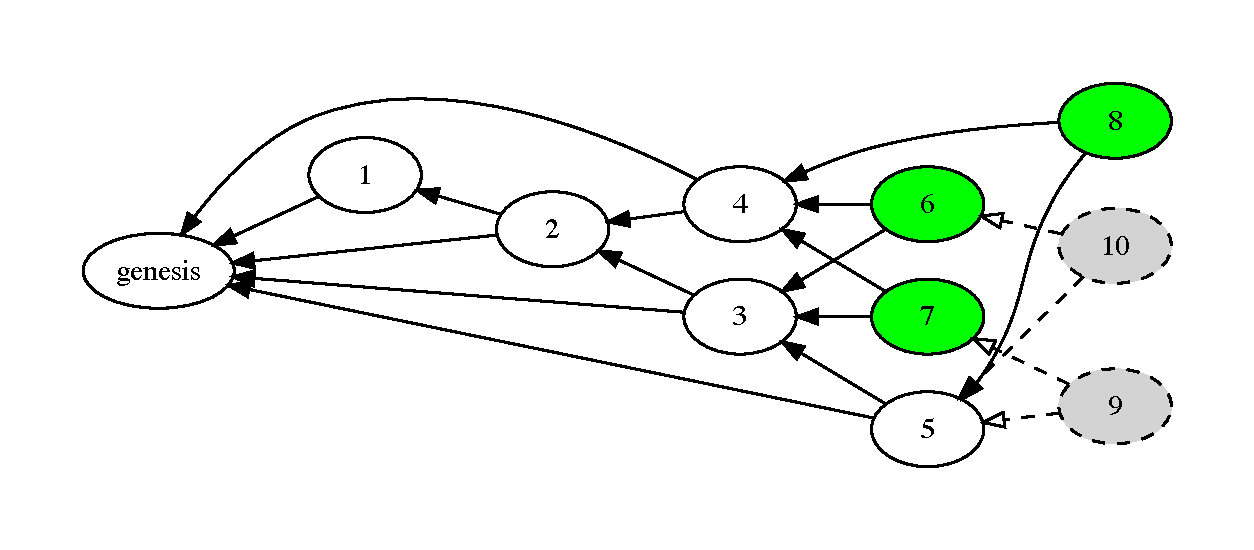
\includegraphics[width=\textwidth]{./images01/fig-tangle-example.pdf}
\caption{White nodes represent transactions that have been confirmed at least once. Green circles represent unconfirmed transactions (tips). Gray and dashed nodes are the transactions currently solving the proof-of-work in order to be propagated.\label{fig-tangle-example}}
\end{figure}

Transactions have an accumulated weight which may be interpreted as how hard it is to rollback a transaction. It is analogous to the number of confirmations of a block in Bitcoin. The higher the accumulated weight, the safer the transaction. Let $A$ be a transaction, its accumulated weight is the sum of all weights of the transactions which confirm $A$, including A itself, i.e., $w_A + \sum_{A \leadsto P} w_P$. For example, in Figure \ref{fig-tangle-example}, the accumulated weight of transaction 3 is the sum of the weights of the transactions 3, 5, 6, 7, and 8.

The score of a transaction is a measure of how much proof-of-work has been done before the transaction has been created. As the heighest score of the network increases over time, comparing a transaction's score with the highest score of the network indicates the ``age'' of the transaction. The score of a transaction A is the sum of all weights of the transactions which are being confirmed by A, including A itself, i.e., $w_A + \sum_{P \leadsto A} w_P$. For example, in Fig. \ref{fig-tangle-example}, the score of transaction 3 is the sum of the weights of the transactions 1, 2, and 3.

Another measure of the ``age'' of a transaction is its height. The height of a transaction A is the length of the longest path from transaction A to the genesis transaction. For example, in Fig. \ref{fig-tangle-example}, the height of transaction 5 is four ($5 \rightarrow 3 \rightarrow 2 \rightarrow 1 \rightarrow$ genesis). The lower the height, the older the transaction.

The depth of a transaction A is a measure of the youth of the transaction. It is the length of the longest path in the inverted graph from transaction A to any unconfirmed transaction (tip). For example, in Fig. \ref{fig-tangle-example}, the depth of transaction 2 is three ($2 \rightarrow 3 \rightarrow 5 \rightarrow 8$). It is the opposite of the height. The lower the depth, the younger the transaction. When a new transaction is confirming two transactions with high depth, it is referred to as lazy transaction.

The higher the volume of new transactions, the more unconfirmed transactions will appear. In Fig. \ref{fig-tangle-swarm}, the reader can notice that the number of new transactions was increased for a while, and then decreased back to the original value. The Iota has behaved well when exposed to a high load scenario, since it reduced the number of tips to only three after the high demand has ceased. It is like a moving swarm which gets wider when the number of new transactions increases and gets thinner when the number of new transactions decreases.

\begin{figure}[ht]
\centering
\includegraphics[width=\textwidth]{./images01/fig-tangle-swarm.pdf}
\caption{Suddenly the number of transactions per second increases and the width of the swarm grows. After a while, the number of transactions per second decreases and the width of the swarm shrinks.\label{fig-tangle-swarm}}
\end{figure}

Conflicting transactions may happen when two or more transactions try to spend the same tokens --- or, in the Bitcoin's transaction format, try to spend the same output. In this case, the network must choose which of the transactions will be accepted and the other one will be invalidated, even when both have already been confirmed. In fact, when one transaction is invalidated, the whole sub-DAG which confirms it is also invalidated. In this case, it may happen to reverse some transactions.

Intuitively, when there is a conflict, the network should accept the transaction which has greater accumulated weight, invalidating the others (see Fig. \ref{fig-tangle-conflict}). But it may be not enough to prevent some attacks like the nuclear submarine attack.

\begin{figure}[ht]
\centering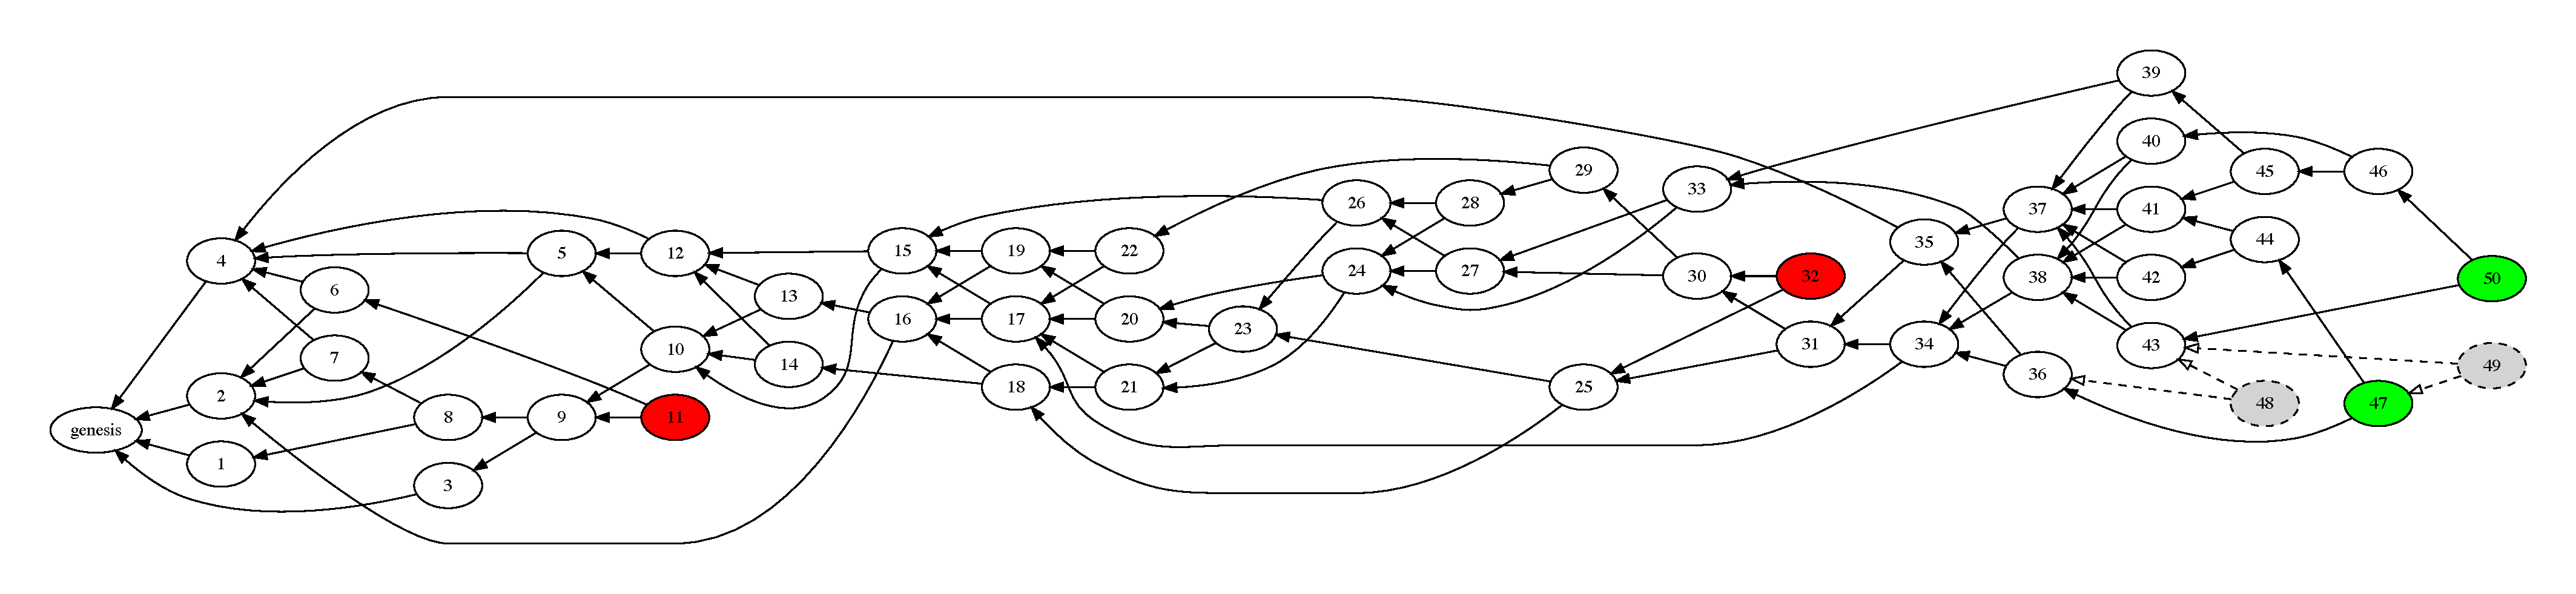
\includegraphics[width=\textwidth]{./images01/fig-tangle-conflict.pdf}
\caption{The red nodes are transactions which had some conflict with previous transaction and were invalidated by the network. Notice that none of them have been confirmed.\label{fig-tangle-conflict}}
\end{figure}

The nuclear submarine attack, also known as the parasite chain attack, is when the attacker generates a separate DAG (or a side DAG), with many transactions and a lot of proof-of-work. This side DAG is off the network, i.e., its transactions have not been propagated. Then, at a convenient moment, the attacker suddenly propagates these transactions. The whole network needs to decide how to handle these transactions.

If the transactions have no conflict with any transaction of the main DAG, i.e., there is no transaction spending the same tokens, then it is easy to handle the transactions. But, as it is an attack, there will be some conflicts, and it is not easy to choose which transaction should be invalidated. As the attacker has been generating a separate DAG, the conflicting transaction may have an accumulated weight similar or greater than the transaction which is already in the main DAG. Hence, using only the accumulated weight may not be enough to prevent this attack.

For example, the attackers generate (and do not propagate) a transaction that transfers all their funds to another address. Then, they start to generate many new transactions which confirm themselves and even confirm some of the transactions in the main DAG, but none of these transactions are also propagated to the network. Afterward, the attacker buys something in the real world, pays with cryptocurrency, and wait until the payment gets the accumulated weight demanded by the merchant. Finally, the attacker suddenly propagates all the transactions to the network in a small window of time. If the criteria is to validate the transaction with higher accumulated weight, the network will accept the attackers' original transaction instead of the one used to pay the merchant. Hence, the merchant transaction is invalidated, and the double spend attack has succeeded.

By default, Iota uses the Markov Chain Monte Carlo (MCMC) algorithm to select the two tips. For further information about attacks and strategies to prevent them, including the MCMC algorithm, see \cite{tangle2016}.


\chapter{Hathor's architecture}
% !TEX root = ../partial-blockchain.tex

This work introduces the Hathor's architecture, which lies between Bitcoin's and Iota's and may be a solution to scaling, centralization, and spam issues.

Like Iota, new transactions confirm previous ones, forming a Directed Acyclic Graph (DAG). For this, each transaction has its own proof-of-work which is solved by the issuer before propagating the transactions in the network. Like Bitcoin, miners find new ``blocks'' every 10 minutes in which they collect the fees and newly generated tokens. Each transaction has an ``accumulated weight'' which express the required effort to break the transaction, similar to Bitcoin's number of confirmations.

In Hathor, there are two difficulty levels: (i) one for new transactions which are just moving tokens around, and (ii) another one for ``blocks'' which are generating new tokens and collecting fees. The first may be adjusted to prevent spammers, which would spend too many resources to generate a great number of new transactions, whereas the latter is adjusted every 2,016 blocks to keep the pace of blocks on every 2 minutes.

Both miners and users will be working on proof-of-work, decentralizing even more the network's hash rate. Even though the users' difficulty is less than the miners', the hash rate will increase with every new user. The more transactions arrive, the higher the total hash rate. This may have good consequences in governance, which we will further discuss.

There is a trade-off about the \textit{difficulty} of new transactions. The higher it is, the harder it is to generate new transactions, preventing spammers but also making it harder for IoT devices generate new transactions. This difficulty may even be increased when a spam attack is in course and reduced when it is gone. If the difficulty is too high, IoT devices may sign their transactions and send them to another devices which have a greater hash rate and will solve their proof-of-work faster.

It also seems interesting to have this difficulty depending on new transaction's size (in bytes) and amount being moved. The idea here is to require more work when high amounts are at stake. It would not affect IoT devices, which are expected to usually move smaller amounts. Regarding the transaction's size, requiring more work for larger transactions may make sense because they may prevent abuses, such as a denial-of-service attack using enormous transactions which would consume a lot of node's bandwidth and disk space.

Another important security matter is that each transaction has to confirm all its inputs, i.e., there must be a confirmation path between all the transactions of the inputs and the transaction which are spending them. It is always possible since there is at least one confirmation path between any transaction and a tip. This ensures that, when a conflict is resolved, only the sub-DAG with root at the invalidated transaction will be affected. The remaining parts of the DAG remains the same.

The transactions are classified into three groups: (i) confirmed transactions, (ii) in-progress transactions, and (iii) unconfirmed transactions (tips). The confirmed transactions are the ones which have already been settled, i.e., their accumulated weights have reached a minimum level. The unconfirmed transactions (tips) are the brand new transactions which have not been confirmed even once yet, i.e., their accumulated weights are zero. The in-progress transactions are in the middle. They have already been confirmed a few times, but not enough to reach the minimum level required to be a confirmed transaction. For simplicity, the pending transactions encompass both in-progress and unconfirmed transactions.

Another transaction classification concerns its validation by the network. A transaction is said to be network validated if there are confirming paths from all tips to the transactions, i.e., the whole network has validated that the transaction is valid. It is important to notice that a transaction may be network validated but still pending, or even be confirmed but not network validated.

A \emph{block} is just a regular transaction with no inputs which confirms a previous block and at least two in-progress transactions or tips. There may be any number of outputs provided that they comply with the number of newly generated tokens. Each block collects all fees from all transactions confirmed by it which have not been confirmed by another block before. The blocks are ordered according to their timestamp. If two blocks have the same timestamp, the block hash is used as a tiebreaker.

In the low load scenario, there is a small number of new transactions coming into the network, which means they give a minor contribution to confirmations. In this case, the confirmation is held mostly by blocks. On the other hand, in the high load scenarios, there is a large number of new transactions giving a major contribution to confirmations. In this case, the blocks strengthen the confirmations, but many of them will have already been confirmed before the next blocks are found. The higher the number of new transactions, the faster the transactions are confirmed. The blocks assure a ``maximum confirmation time''.

The incentive scheme which keeps the network running is the same as Bitcoin's. Miners go towards fees and newly generate coins, whereas users just want to exchange their tokens. When there is no new transaction to be confirmed, the miners keep the network up and running while they find new blocks.


\section{Transaction confirmation}

Hathor uses similar concepts of weight and accumulated weight as Iota's. The weight depends only in the transaction itself, whereas the accumulated weight depends on its confirmations.

The weight of a transaction is calculated as $w = \log_2(k)$ where $k$ is the average number of hashes required to solve its proof-of-work.

The accumulated weight is the average number of hashes required to solve the proof-of-work of the transaction itself plus all the transactions which confirm it. Let $A$ be a transaction, its accumulated weight $w_A$ is calculated as $\log_2(2^{w_A} + \sum_{A \leadsto P} 2^{w_P})$.

In Bitcoin, it is well-known that one should wait at least ``six confirmations'' before accepting a transaction. This Bitcoin's criteria is based on some math presented in Satoshi's seminal work \citep{nakamoto2008bitcoin}. Adopting six confirmations is the same as demanding from attackers a minimal effort of six times the network's hash rate to successfully double spend those tokens. Let $H$ be the total hash rate of the network. Then, as $\mathbf{E}(Y_6) = 60 \text{ minutes}$, it will be necessary to calculate, on average, $\mathbf{E}(Y_6) \cdot H = 60 \cdot 60 \cdot H$ hashes to solve the proof-of-work of 6 blocks.

Therefore, in order to have the same level of security as Bitcoin, a transaction is said to be confirmed when its accumulated weight is greater than or equal to $\log_2(\mathbf{E}(Y_6) \cdot H) = \log_2(6 \cdot 128 \cdot H) = 7 + \log_2(6) + \log_2(H)$, where $H$ is calculated as the total hash rate of the miners plus the total hash rate of new transactions.


\section{Time between blocks}

The hash function used for the proof-of-work (PoW) is the same as Bitcoin: \emph{SHA-256} applied twice. Thus, most of the math analysis we have already done before is just the same.

Let $X$ be the number of trials to solve the PoW and $T$ be the time between blocks. We already know that $X$ follows a geometric distribution with $p = \frac{A}{2^{256}}$, where $A$ is inversely proportional to the difficulty, i.e., the smaller the $A$, the higher the difficulty. We also know that $T$ follows an exponential distribution with $\lambda = \frac{1}{\eta}$, where $\eta$ is the average time between blocks. As proved before, $\eta p H = 1$, thus let's define $w = \log_2(\mathbf{E}(X)) = \log_2(1/p) = \log_2(\eta H) = \log_2(\eta) + \log_2(H)$.

For the blocks, $\eta = 128$, thus, $\mathbf{E}(T) = 128 \text{ seconds}$, and $\mathbf{V}(T) = 16,384$. The symmetrical confidence interval with $\alpha = 10\%$ is $[6.56, 383.45]$, i.e., 90\% of the cases the distance between blocks will be between 6 seconds and just under 7 minutes.

Let $H$ be the hash rate of the miners, then, the weight of the blocks is calculated by

$$w_\text{blocks} = \log_2(128) + \log_2(H) = 7 + \log_2(H)$$

This weight will be updated every 2,016 blocks to take into consideration the change of $H$. First, $H$ will be estimated using the fact that $\mathbf{E}(Y_{2016}) = \frac{2016}{\lambda} = 2016 \eta = \frac{2016}{pH} = \frac{2016 \cdot 2^w}{H}$. Thus, $H = \frac{2016 \cdot 2^w}{\Delta t} \Rightarrow \log_2(H) = w + \log_2(2016) - \log_2(\Delta t)$, where $\Delta t$ is the time between the latest weight update and now. Finally,

$$w_\text{new} = 7 + w_\text{old} + \log_2(2016) - \log_2(\Delta t)$$

Notice that, if the hash rate has not changed, then $\Delta t = 128 \cdot 2016$ and $w_\text{new} = w_\text{old}$.


\section{Weight of the transactions}

There is a trade-off which must be considered in the weight of the transactions: the higher the weight, the better to prevent spam, but the worse to microtransactions. So, trying to fulfill both necessities, the weight will be a function of the transaction's size (in bytes) and total amount:

$$w_\text{tx} = \log_2(\text{size}) + \log_2(\text{amount}) + 0.5$$

Although the transaction size depends on the implementation, a typical transaction with 2 inputs and 2 outputs would have approximately 188 bytes. So, for instance, transfering 50,000 tokens would require a weight of 23, which means an average of $2^{23}$ trials to solve the proof-of-work.


\section{Issuance rate}

Hathor issues tokens every block, thus it is similar to Bitcoin. Even so, an important decision is whether it will issue a limited number of tokens or not. Bitcoin chose to issue a limited number of tokens. On the other hand, Ethereum and others chose to issue an ilimited number of tokens.

Both ways, the number of issued tokens is predictable. This feature itself brings confidence to the community, who will not face monetary intervention (unless they agree to) --- this comes in contrast with fiat money in which the central authority may change the monetary policy to adjust to political demands.

Bitcoin issuance rate started in 50 tokens per block and decreases over time. Every 210,000 blocks---4 years, on average---it halves the number of tokens issued per block. As Bitcoin smallest fraction is $10^{-8}$, after the 33th reduction it will stop issuing new tokens since $2^{33} > 50 \cdot 10^{-8}$. In total, the number of issued tokens will never exceed 21 million. For further information, see \cite{bitcoinsupply}.

%Using the same strategy, Hathor's issuance rate starts in 50,000 tokens per block and decreases over time. Different from Bitcoin, Hathor's tokens are always integers and cannot be split. Every 1,000,000 blocks, the number of tokens issued per block is halved. Thus, the supply is limited to 100 billion issued tokens during its whole life. To calculate the supply limit use the following equation:

%\begin{align*}
%    \sum_{k=0}^{\infty} 1,000,000 \cdot \left\lfloor \frac{50000}{2^k} \right\rfloor \approx
%    \sum_{k=0}^{\infty} 1,000,000 \cdot \frac{50000}{2^k} = 100 \text{ billion}
%\end{align*}

%As the average time between blocks is 128 seconds, it will take around 3 years, 9 months and 20 days between halves.


\section{Transaction fees}

In Bitcoin, the value of the fee is calculated as the difference between the transaction's outputs and the inputs. For instance, a transaction with inputs summing 8,000 and outputs summing 7,000 is paying 1,000 of fees.

In Hathor, each transaction may pay a fee to the next block which confirms it. But, even if the fee is zero, the miners are forced to confirm at least two pending transactions. These two pending transactions also confirm other transactions which may have no fees. In summary, transactions with no fees cannot be left behind and will always be confirmed by both blocks and other transactions.

One may arguee that it allows the whole network to never pay fees and they are right. In the beginning, miners' incentive is driven by new tokens instead of fees. In the long term, it may be necessary to require a minimum fee to keep the miners working, depending on the chosen issuance policy.


\section{Transaction validation}

A transaction will be considered valid when it complies with the following rules: (i) it spends only unspent outputs; (ii) the sum of the inputs is greater than or equal to the sum of the outputs; (iii) the number of inputs is at most 256; (iv) the number of outputs is at most 256; (v) it confirms at least two pending transactions; (vi) it solves the proof-of-work with the correct weight.

The transaction has a timestamp field which is used to record when the transaction was generated. This timestamp field must be in UTC time to prevent timezone issues. It must also be within at most 5 minutes from the current time, otherwise the transaction will be discarded.

The digital signature is used to ensure that only the owners may spend their tokens. It will be calculated signing the transaction's input and output only. This allows the transaction to be signed in one device and to be sent to another device that will choose which transaction will be confirmed and will solve the proof-of-work.

Services of solving proof-of-work may also be offered by companies. They give their customers a wallet address and they send the payment inside of the transaction itself. This allows IoT devices to save energy, delegating the task of solving the proof-of-work.

In case of transaction conflict, in which two transactions try to spend the same tokens, the one with higher accumulated weight is chosen and the other is invalidated. Although it is not a possible policy in Iota because of the submarine attack, Hathor does not have the same problem. In Hathor, like in Bitcoin, the submarine attack is only possible if the attacker has a hash rate higher than the whole network, including the miners. In other words, when analysing the double spending attack, Hathor is as safe as Bitcoin.


\section{Orphan blocks}

Different from Bitcoin, there is no orphan blocks in Hathor. Unless a block confirms either directly or indirectly an invalid transaction, every block is valid. There is no need to left a block behind since its proof-of-work is increasing transactions' accumulated weight.

If two blocks are trying to collect fees from the same transactions, the one with higher timestamp will be discarded.


\section{Governance}

In general, cryptocurrencies are decentralized, which means there is no central authority who decides its future, i.e., no one can enforce their will. Every decision must be accepted by its community, which means the community must agree. But what happens if they do not agree? When a consensus is not reached, the rules remain the same and the cryptocurrency may stall. The lack of a central authority may generate long debates, split the community, slow down strategic decision-making, and, ultimately, come to a ``civil war''---it is precisely what happened between Bitcoin Core (BTC) and Bitcoin Cash (BCH) in 2017 \citep{bloomberg2017civilwar, forbes2017civilwar}.

Governance is an important part of a cryptocurrency because it must evolve, which means its community must agree into changing the rules. Governance is an agreement of how the community will proceed to change the rules.

Despite the large literature available about governance, what separates Blockchain-based cryptocurrencies from them is the decentralization (against the hierarchical model). The number of papers about governance in decentralized cryptocurrencies has been growing, but it still lacks a solution. \citet{hacker2017corporate} resorts to the theory of complex systems and proposes a governance framework for decentralized cryptocurrencies, which is, in summary, a centralized coordination entity. \citet{hsieh2017internal} has analyzed the effects of governance in returns using panel data on several cryptocurrencies. They present a deeper discussion about the parts of a governance mechanism and concludes that

\begin{quote}
``... on the one hand, investors value cryptocurrencies’ core value proposition, rooted in decentralization; but on the other hand, are suspicious of decentralized governance at higher levels in the organization because they could slow down strategic decision-making (e.g., regarding the introduction of new innovations) or create information asymmetries between investors and technologists.''
\end{quote}

I believe that the solution to a good governance will come from financial incentives to all players to find a common ground. In Bitcoin, users have less bargaining power than miners because they do not contribute with work, whereas, in Hathor, both miners and users are working together. So, when it comes to changing the rules, the bargaining power is more distributed than in Bitcoin. The distribution depends on the ratio of the miners' hashpower and the users' hashpower. The higher the ratio, the closer to Bitcoin's governance. The lower the ratio, the higher the bargaining power of the users.

%- Punishment for miners/transactions which does not comply with the rules.
%- Rule change policy.

\section{Expected number of tips}

It is intuitive that the number of tips depends on the number of transactions per second. The higher the number of transactions per second, the higher the number of tips. We can model the number of tips at time $t$ as a stochastic process, which means it changes over time following some probability distribution. Stochastic processes have two important states: transient and steady. A process is in transient state when its properties are changing over time, whereas it is in steady state when its properties has already converged.

Let's assume that the number of transactions per second is constant and does not change over time. Thus, at the beginning, there will be no tips, and the number will increase until it converges to its stable quantity. The process is in transient state until it reaches stability. Then, it is in the steady state. Notice that the number of tips also change in steady state, but its average does not. It just floats around the average.

If the number of transactions per second increases, the process returns to the transient state and moves towards the new steady state. In practice, the number of transactions per second is always changing, so is the steady state.

\citet{tangle2016} has modeled the stochatic process of the total number of tips. It proves that the average number of tips, in the steady state, is:

$$\frac{\lambda_\text{TX} \cdot 2^{w_\text{TX}}}{\log(2)H}$$

A simple idea to get to this equation is through flow analysis: In steady state, we may say that the number of new tips must equal the number of tips being confirmed in a given time window. Thus, in order to estimate the number of tips in the steady state, let's consider the process in which the rate of inward tips is $\lambda_\text{TX}$, whereas the rate of outward tips is $\rho$.

Let $K$ be the number of tips at a given time. Thus, after $\Delta t$ seconds, $\Delta \text{tips} = \lambda_\text{TX} \Delta t - \rho K \Delta t$. In the steady state, $\Delta \text{tips} = 0$, hence $K = \frac{\lambda_\text{TX}}{\rho}$.

The rate of outward tips is proportional to the rate in which devices solve the proof-of-work of transactions. Let $H$ be the devices' hash rate, then, $\rho = \alpha \cdot H \cdot 2^{-w_\text{TX}}$, where $\alpha$ is the coefficient of proportionality.

Finally,

$$K = \frac{\lambda_\text{TX}}{\alpha} \frac{2^{w_\text{TX}}}{H}$$

If new transactions would always confirm two tips, then $\alpha$ would equal 2. But, it may confirm one or even zero tips because concurrent new transactions may confirm their tips first. Thus, $0 < \alpha \le 2$. According to the equation found in \citet{tangle2016}, $\alpha = \log(2) = 0.693147$.

%$$\frac{\lambda_\text{TX} \cdot 2^{w_\text{TX}}}{2H} \le K \le \frac{\lambda_\text{TX} \cdot 2^{w_\text{TX}}}{H}$$

%\section{Attacks \& Conflicting transactions}
%\section{Scripts \& Contracts}
%\section{Bandwidth consumption}


\section{Governance}

- Punishment for miners/transactions which does not comply with the rules.

- Rule change policy.


\section{Expected number of tips}

Explain transient and stationary state. The balance happens in the stationary state.

In order to estimate the balance in the number of tips, let's consider the system in which the rate of inward tips is $\lambda_\text{TX}$, while the rate of outward tips is $\rho$. Let $K$ be the number of tips in the system. Thus, after $\Delta t$ seconds, $\Delta \text{tips} = \lambda_\text{TX} \Delta t - \rho K \Delta t$. In the balance, $\Delta \text{tips} = 0$, hence $K = \frac{\lambda_\text{TX}}{\rho}$.

Finally, the rate of outward tips is twice the rate in which devices solve the proof-of-work of transactions. Let $H$ be the devices' hash rate, then, $\rho = 2 \cdot H \cdot 2^{-w_\text{TX}}$.

Twice?! It is a number between 1 and 2, but none of them.

Therefore, in the balance,

$$K = \frac{\lambda_\text{TX} \cdot 2^{w_\text{TX}}}{2H}$$

$$\frac{\lambda_\text{TX} \cdot 2^{w_\text{TX}}}{2H} \le K \le \frac{\lambda_\text{TX} \cdot 2^{w_\text{TX}}}{H}$$


\section{Attacks \& Conflicting transactions}


\section{Scripts \& Contracts}



\chapter{Methodology}

The methodology we have used is computer simulation. Through the simulation of many scenarios of Hathor, we will understand how the network behaves in complex scenarios, including when the load suddenly increases, and when the network is under attack.

The simulator has been developed using an event-based design which is capable of running hours of simulation in just a few minutes. It creates agents who decide to make a transaction, then they select which transactions will be confirmed, then they spend some time working in the proof-of-work, and, finally, they propagate the transaction to the network. The other agents receive the transaction and may accept or deny it. The agents may use different parameters among themselves.

When a new transaction emerges, it chooses two tips to confirm before solving the proof-of-work. When it finishes solving the proof-of-work, it is propagated and becomes a tip. So, two new transactions may choose the same tips to confirm. If there are $t$ tips, a new transaction will randomly choose 2 out of these $t$ tips, even if they have already been chosen by other new transactions --- in fact, they do not know which have been chosen because these new transactions have not being propagated yet.

When a new transaction is added to the Hathor's network, it uses a depth-first search \citep{cormen2009introduction} (i) to update the aggregated weight of the directly and indirectly confirmed transactions, (ii) to calculate its own score, and (iii) to generate a topological sort \citep{cormen2009introduction}. The topological sort is used to calculate the longest path from all other transactions to the new transaction, and this longest path is used to update the depth of the whole DAG. If the new transaction confirms only transactions which has already been confirmed, the depth update is skipped thanks to Theorem \ref{theorem-new-tx-not-tip}.

The amount of time spent to solve the proof-of-work is a sample from an exponential distribution.

The time between two new transactions is sampled from an exponential distribution with parameter $\lambda$. The value of $\lambda$ is changed over time, causing changes in the load of the network. We consider 1 tx/s to be a low load, and 15 tx/s to be a high load. Even though we have already tested up to 100 tx/s.

The simulator will output different reports: (i) snapshots of the DAG at interesting moments, such as Fig. \ref{fig-tangle-example}, \ref{fig-tangle-swarm}, and \ref{fig-tangle-conflict}; (ii) histogram of confirmation time, such as Fig. \ref{fig-tangle-hist} and \ref{fig-tangle-hist-2}; and many others.


\chapter{Analysis of Hathor}

Hathor's architecture lies between Iota and Bitcoin's architectures. It is similar to Bitcoin's architecture when the number of transactions per second is low, while it is similar to Iota's architecture when the number of transactions per second is high. In order to check this statement, I have run some simulations.

First, two simulations with the extreme cases: (i) no miners, (ii) no transactions. The first should have exactly the same behavior as Bitcoin's blocks with one block after the other forming a long chain. The latter should have a similar behavior as Iota's structure, forming a Direct Acyclic Graph (DAG) with transactions confirming transactions. We can notice in Figure \ref{fig:hathor-similarities} that both cases seem to be correct.

Then, I have run a simulation with both miners and transactions. As we can see in Figure \ref{fig:hathor-dag}, Hathor's structure is a mix of Iota and Bitcoin's structure. The transactions are forming a DAG while, in parallel, the blocks are forming a chain. Differently from Bitcoin, there is no orphan block which means some blocks may be found close to the previous one.

\begin{figure}[!htb]
\centering
\subfloat[No miners]{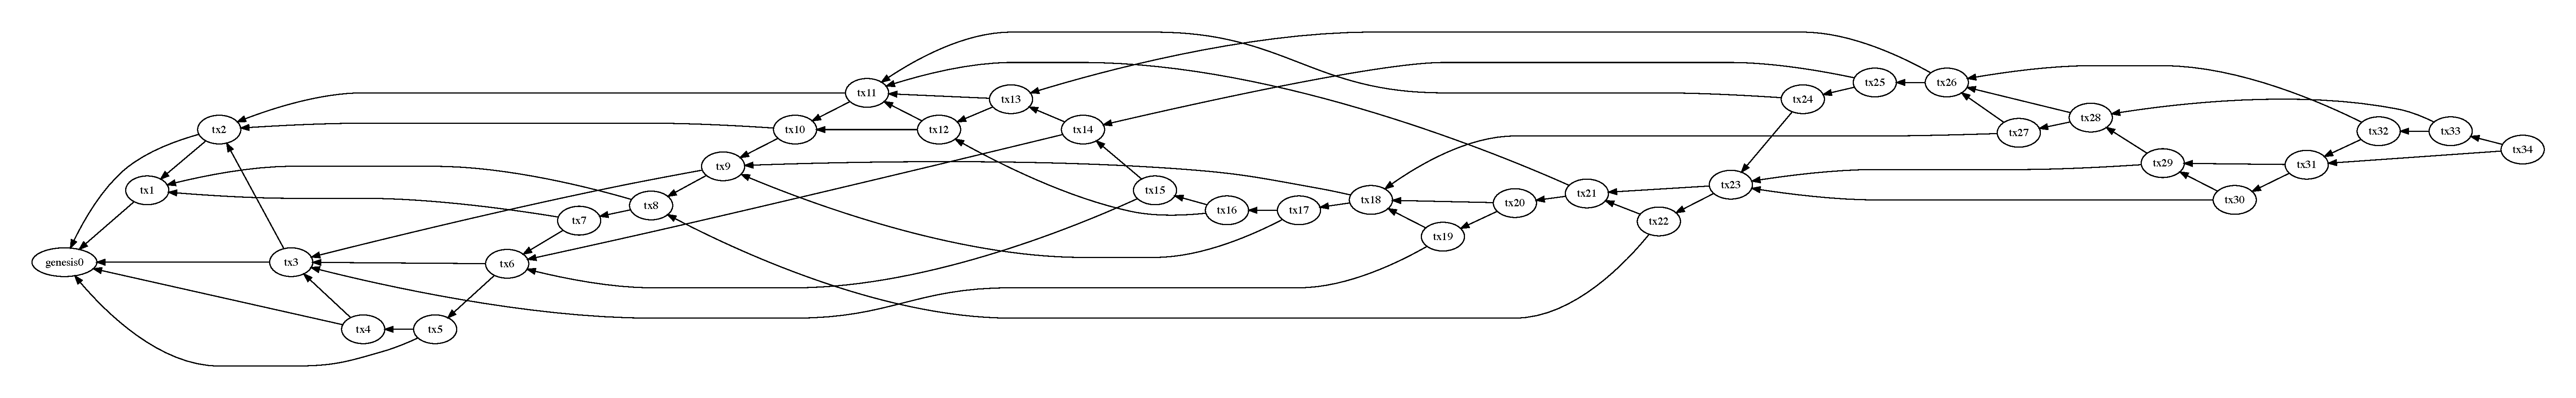
\includegraphics[width=0.5\textwidth]{./images01/sim/no_miners.pdf}}
\subfloat[No transactions]{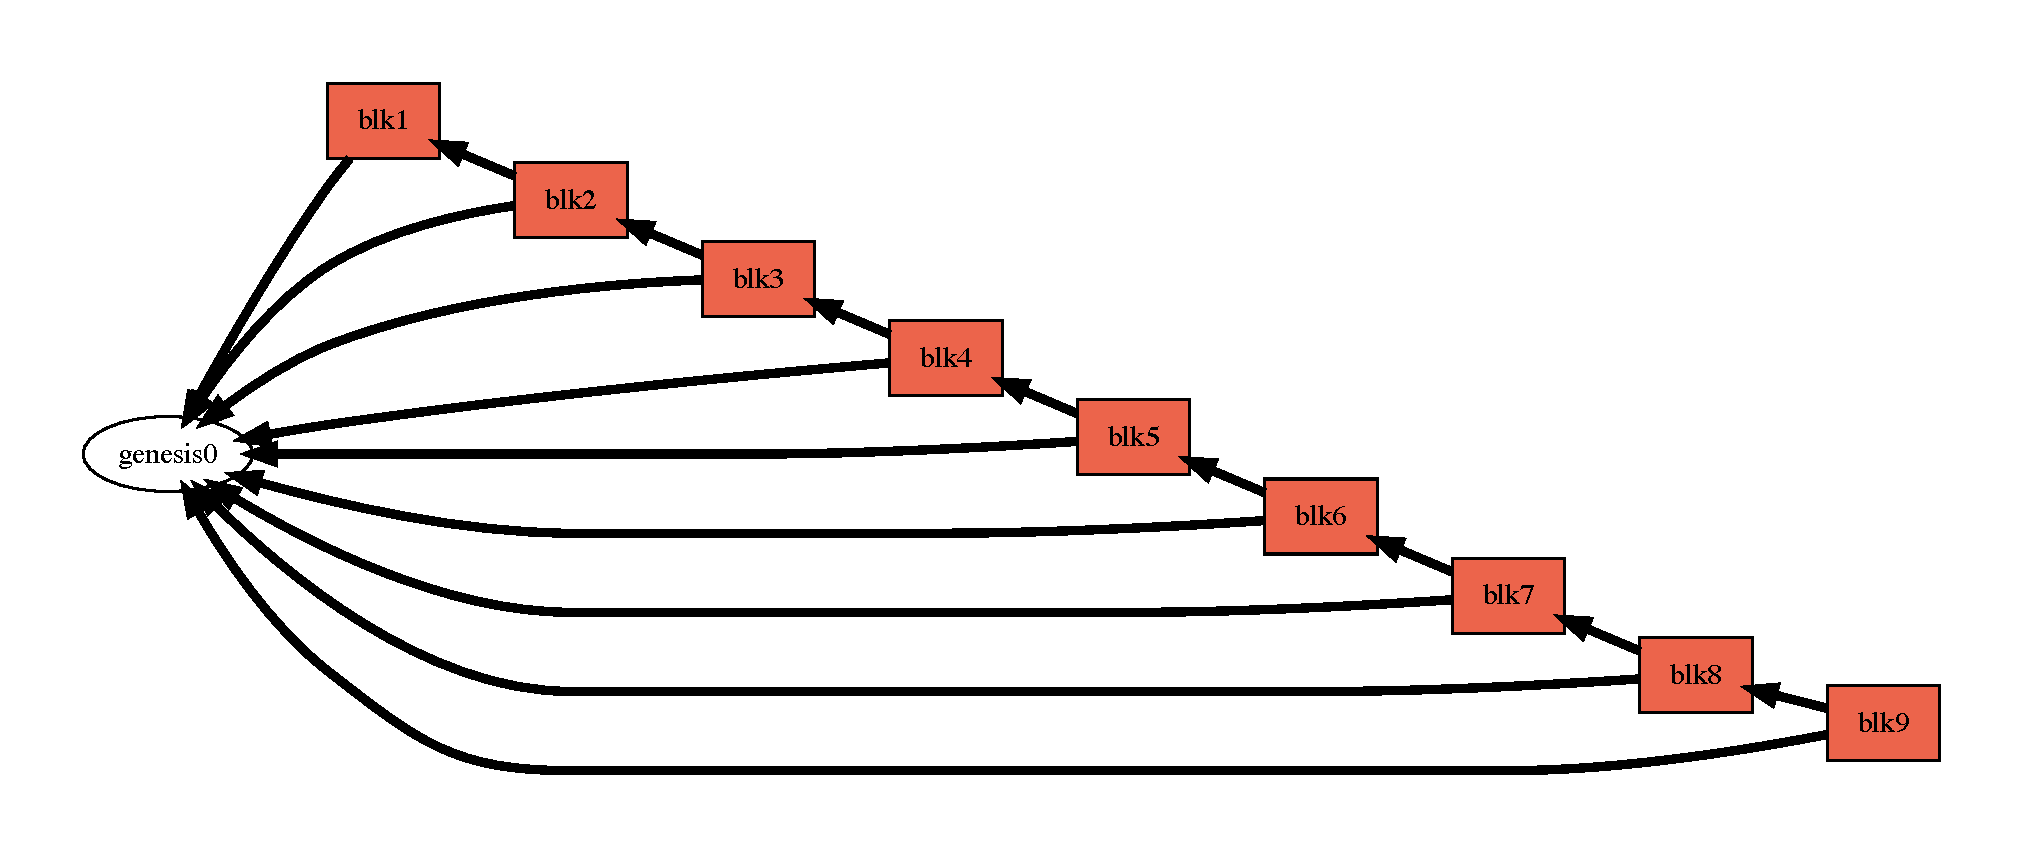
\includegraphics[width=0.5\textwidth]{./images01/sim/only_miners.pdf}}
\caption{Visualization of a Hathor's graph in two particular cases: (a) no miners, (b) no transactions. It shows that when there are no miners, Hathor is similar to Iota (same structure, but different parameters), and when there is no transactions, it is similar to Bitcoin.\label{fig:hathor-similarities}}
\end{figure}

\begin{figure}[!htb]
\centering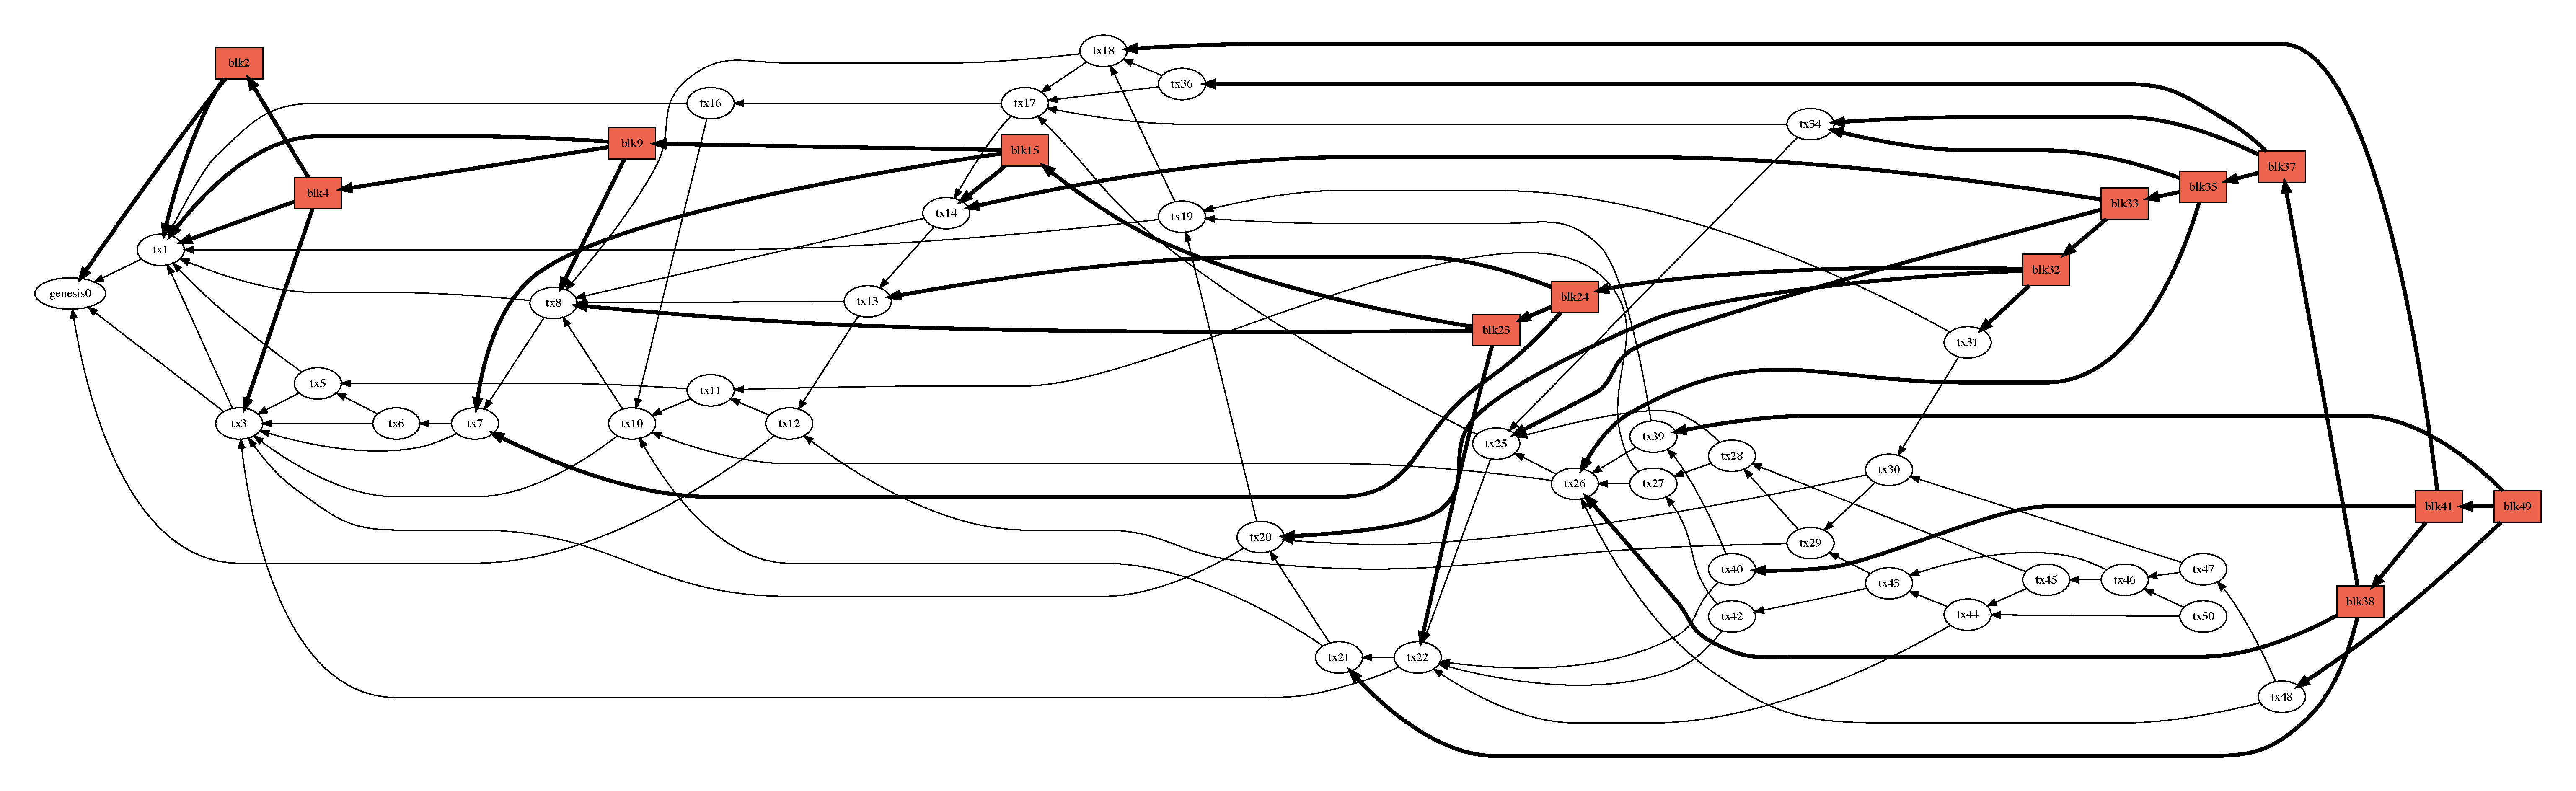
\includegraphics[width=\textwidth]{./images01/sim/hathor.pdf}
\caption{Visualization of a Hathor's graph with transactions and blocks. Red boxes are blocks, and white circles are simple transactions. The arrows show the confirmations.\label{fig:hathor-dag}}
\end{figure}


Another evidence that Hathor lies between Iota and Bitcoin is found when comparing the time to confirm a transaction. In this context, a transaction is said to be confirmed when it has reached an accumulated weight similar to six times the hash rate of the whole network (miners and new transactions). This criteria is equivalent to the well-known ``6 confirmations'' of Bitcoin, which is adopted by almost the whole network.

Thus, I have run a simulation in which miners are majority and there are few transactions. In Figure \ref{fig:hathor-tct-low-mid}, we may see a good fit between the confirmation time of a transaction and the theoretical distribution of the time to find six blocks in Bitcoin (which is $Y_6$ and follows an Erlang distribution). When the load is increased, Hathor's confirmation time is reduced and diverges from Bitcoin's distribution. The reasoning is that confirmations coming from other transactions start to play an important role and accelerates the speed of confirmations.

\begin{figure}[!htb]
\centering
\subfloat[Low load]{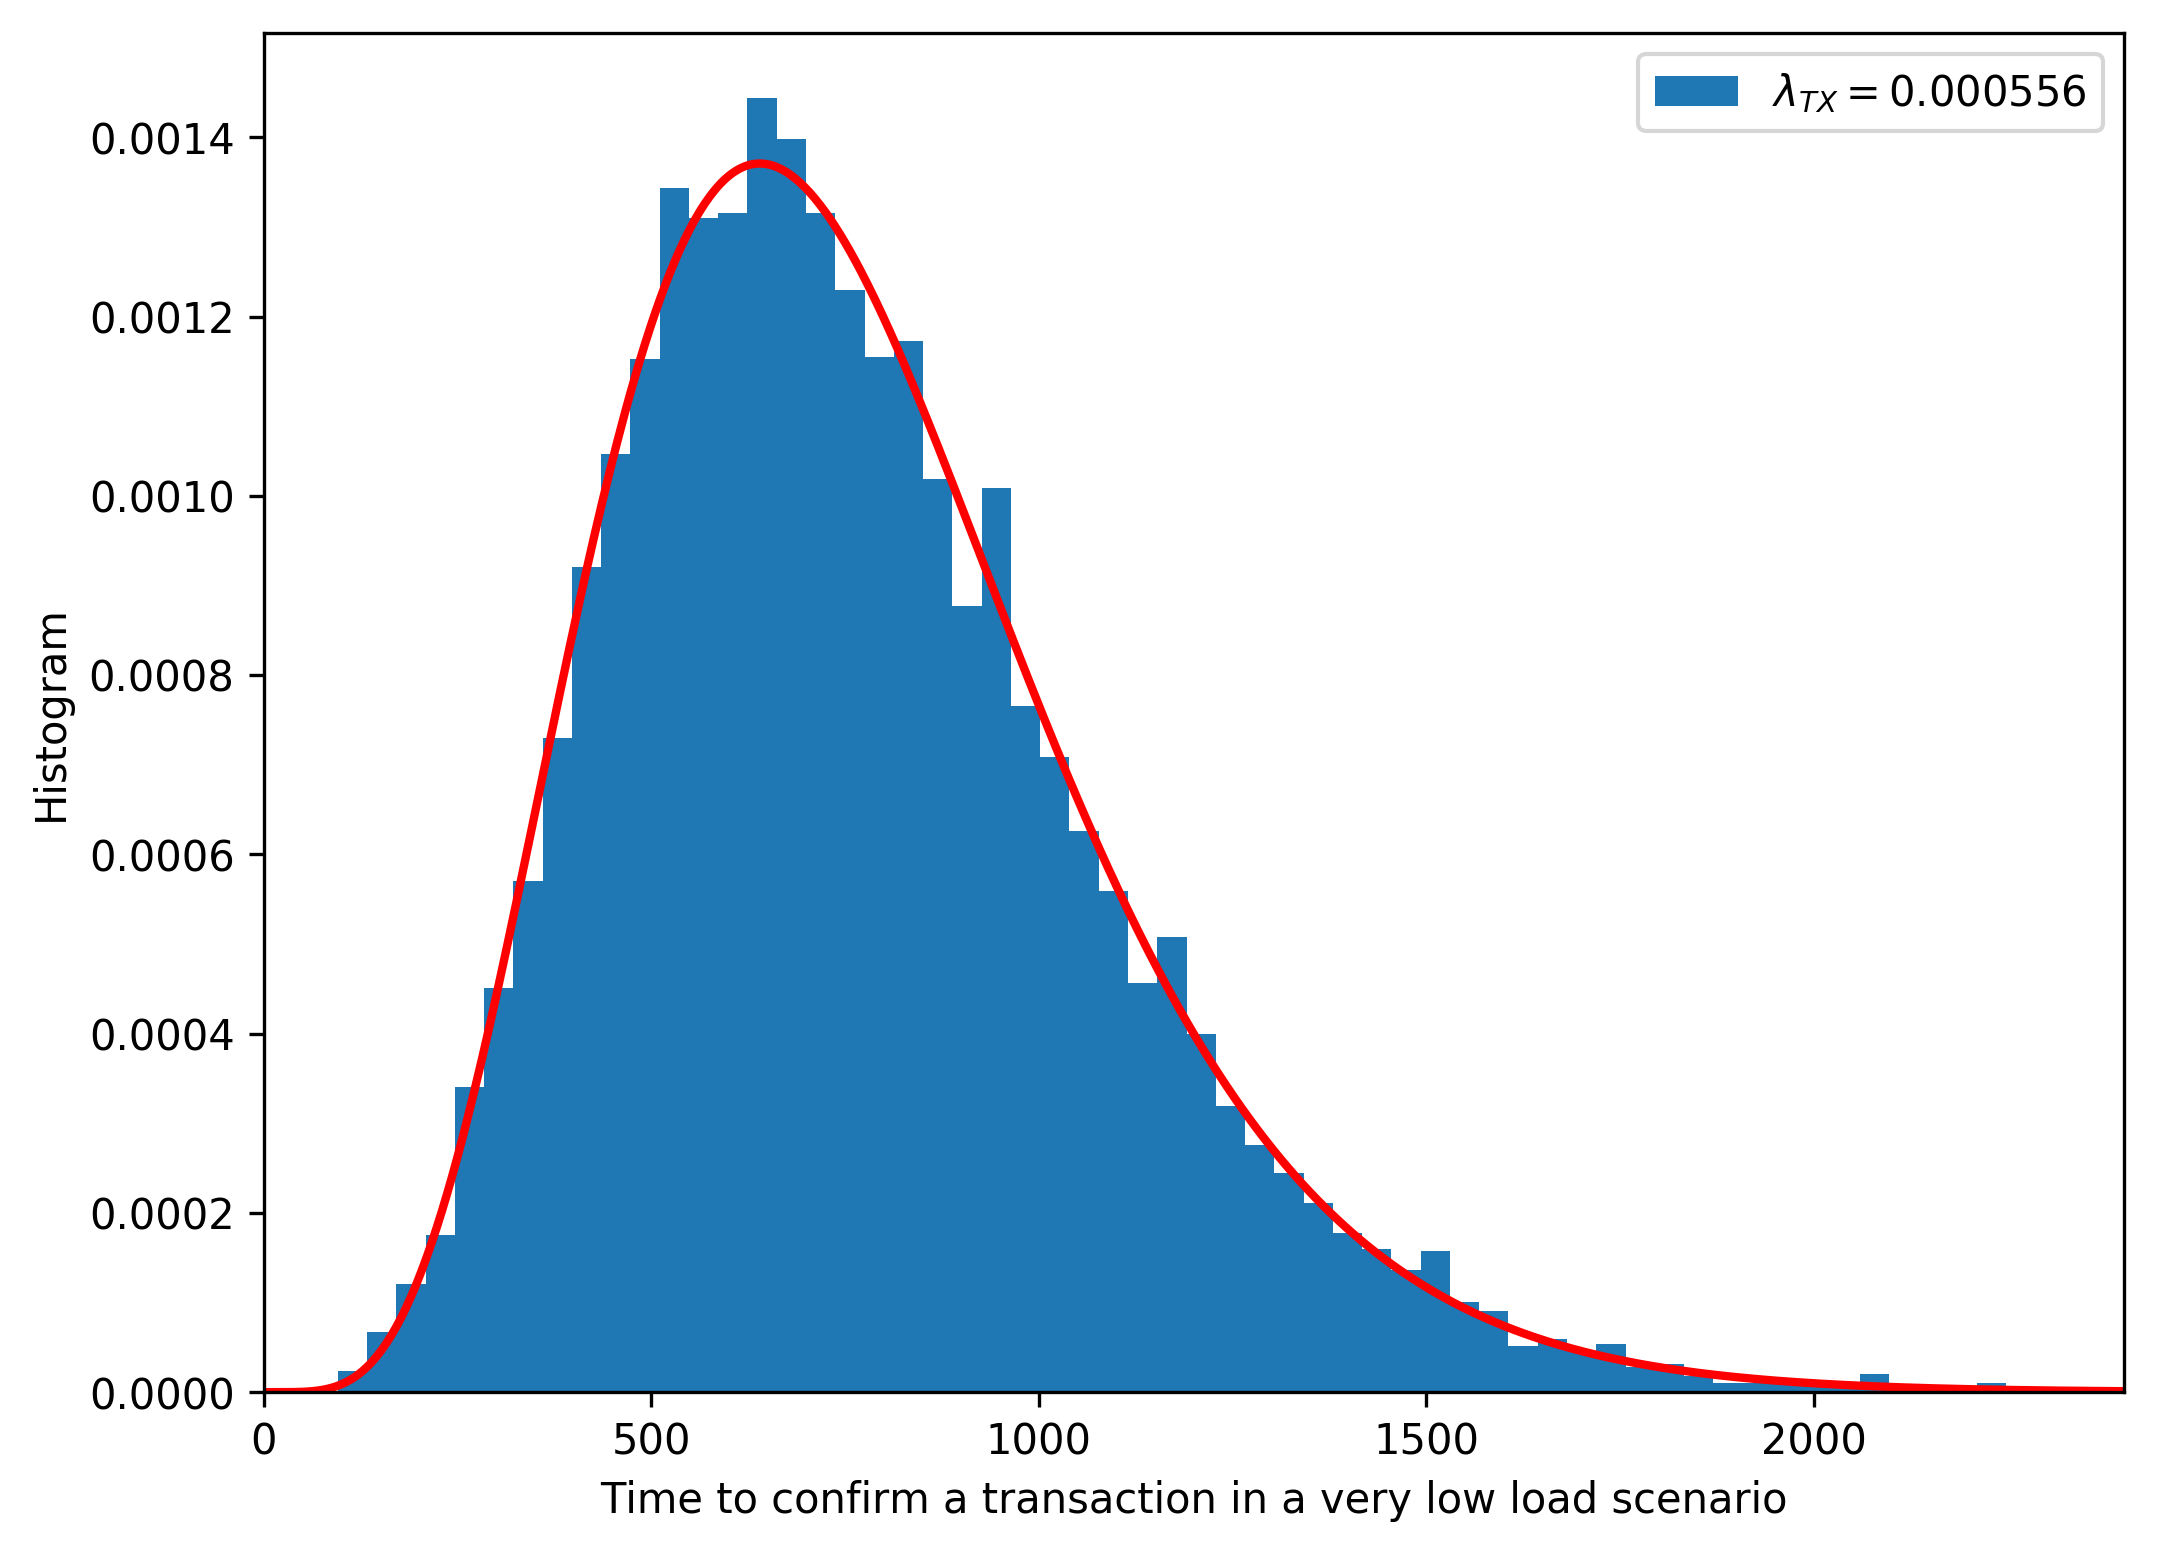
\includegraphics[width=0.5\textwidth]{./images01/sim/tct-low-load.png}}
\subfloat[Mid load \label{fig:hathor-tct-mid-load}]{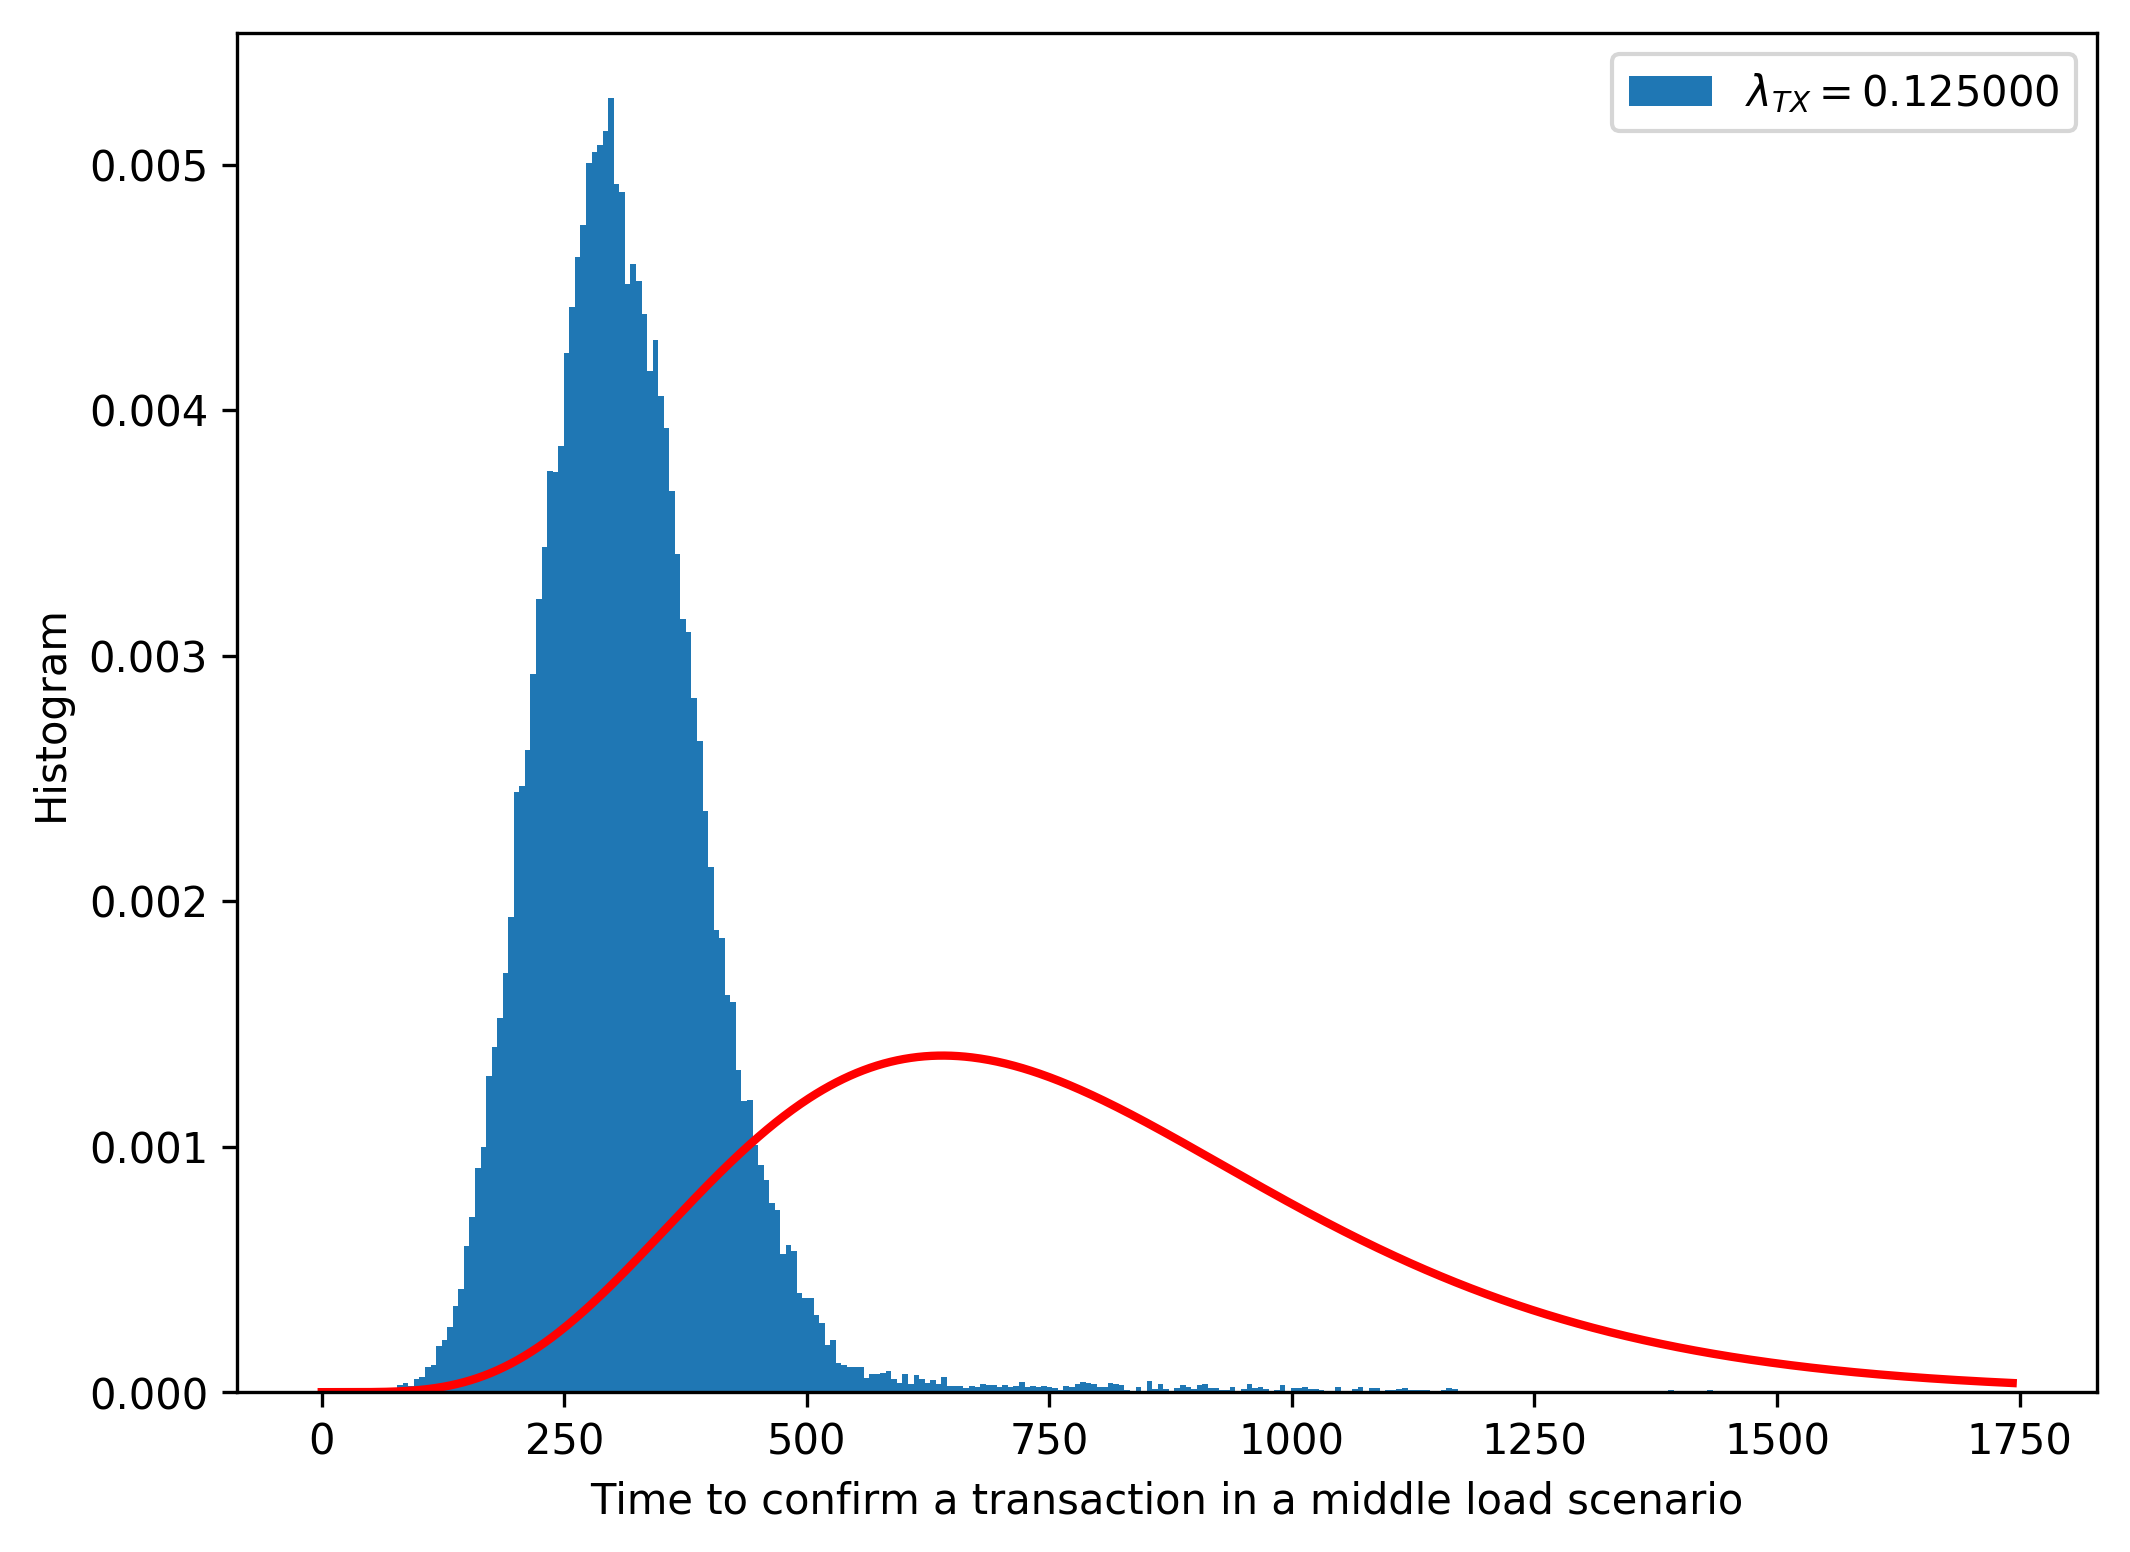
\includegraphics[width=0.5\textwidth]{./images01/sim/tct-mid-load.png}}

\caption{Confirmation time in two scenarios: (a) low load, (b) mid load. The red curve is the distribuion of the time to find six blocks in Bitcoin (which follows an Erlang distribution). As we can notice, in the low load scenario, Hathor's confirmation time behaves just like Bitcoin's. When the load is increased, it starts to diverge from Bitcoin's distribution. \label{fig:hathor-tct-low-mid}}
\end{figure}

We may see Hathor's confirmation time moving from Bitcoin's to Iota's in Figure \ref{fig:hathor-tct-many}. Notice that the confirmation timer is getting smaller as the number of transactions per second increases. Figure \ref{fig:hathor-tct-many-right} is a zoom-in in the right side, and we can see again the good fit between Hathor Bitcoin's confirmation time under low load.

\begin{figure}[!htb]
\centering
\subfloat[The whole picture]{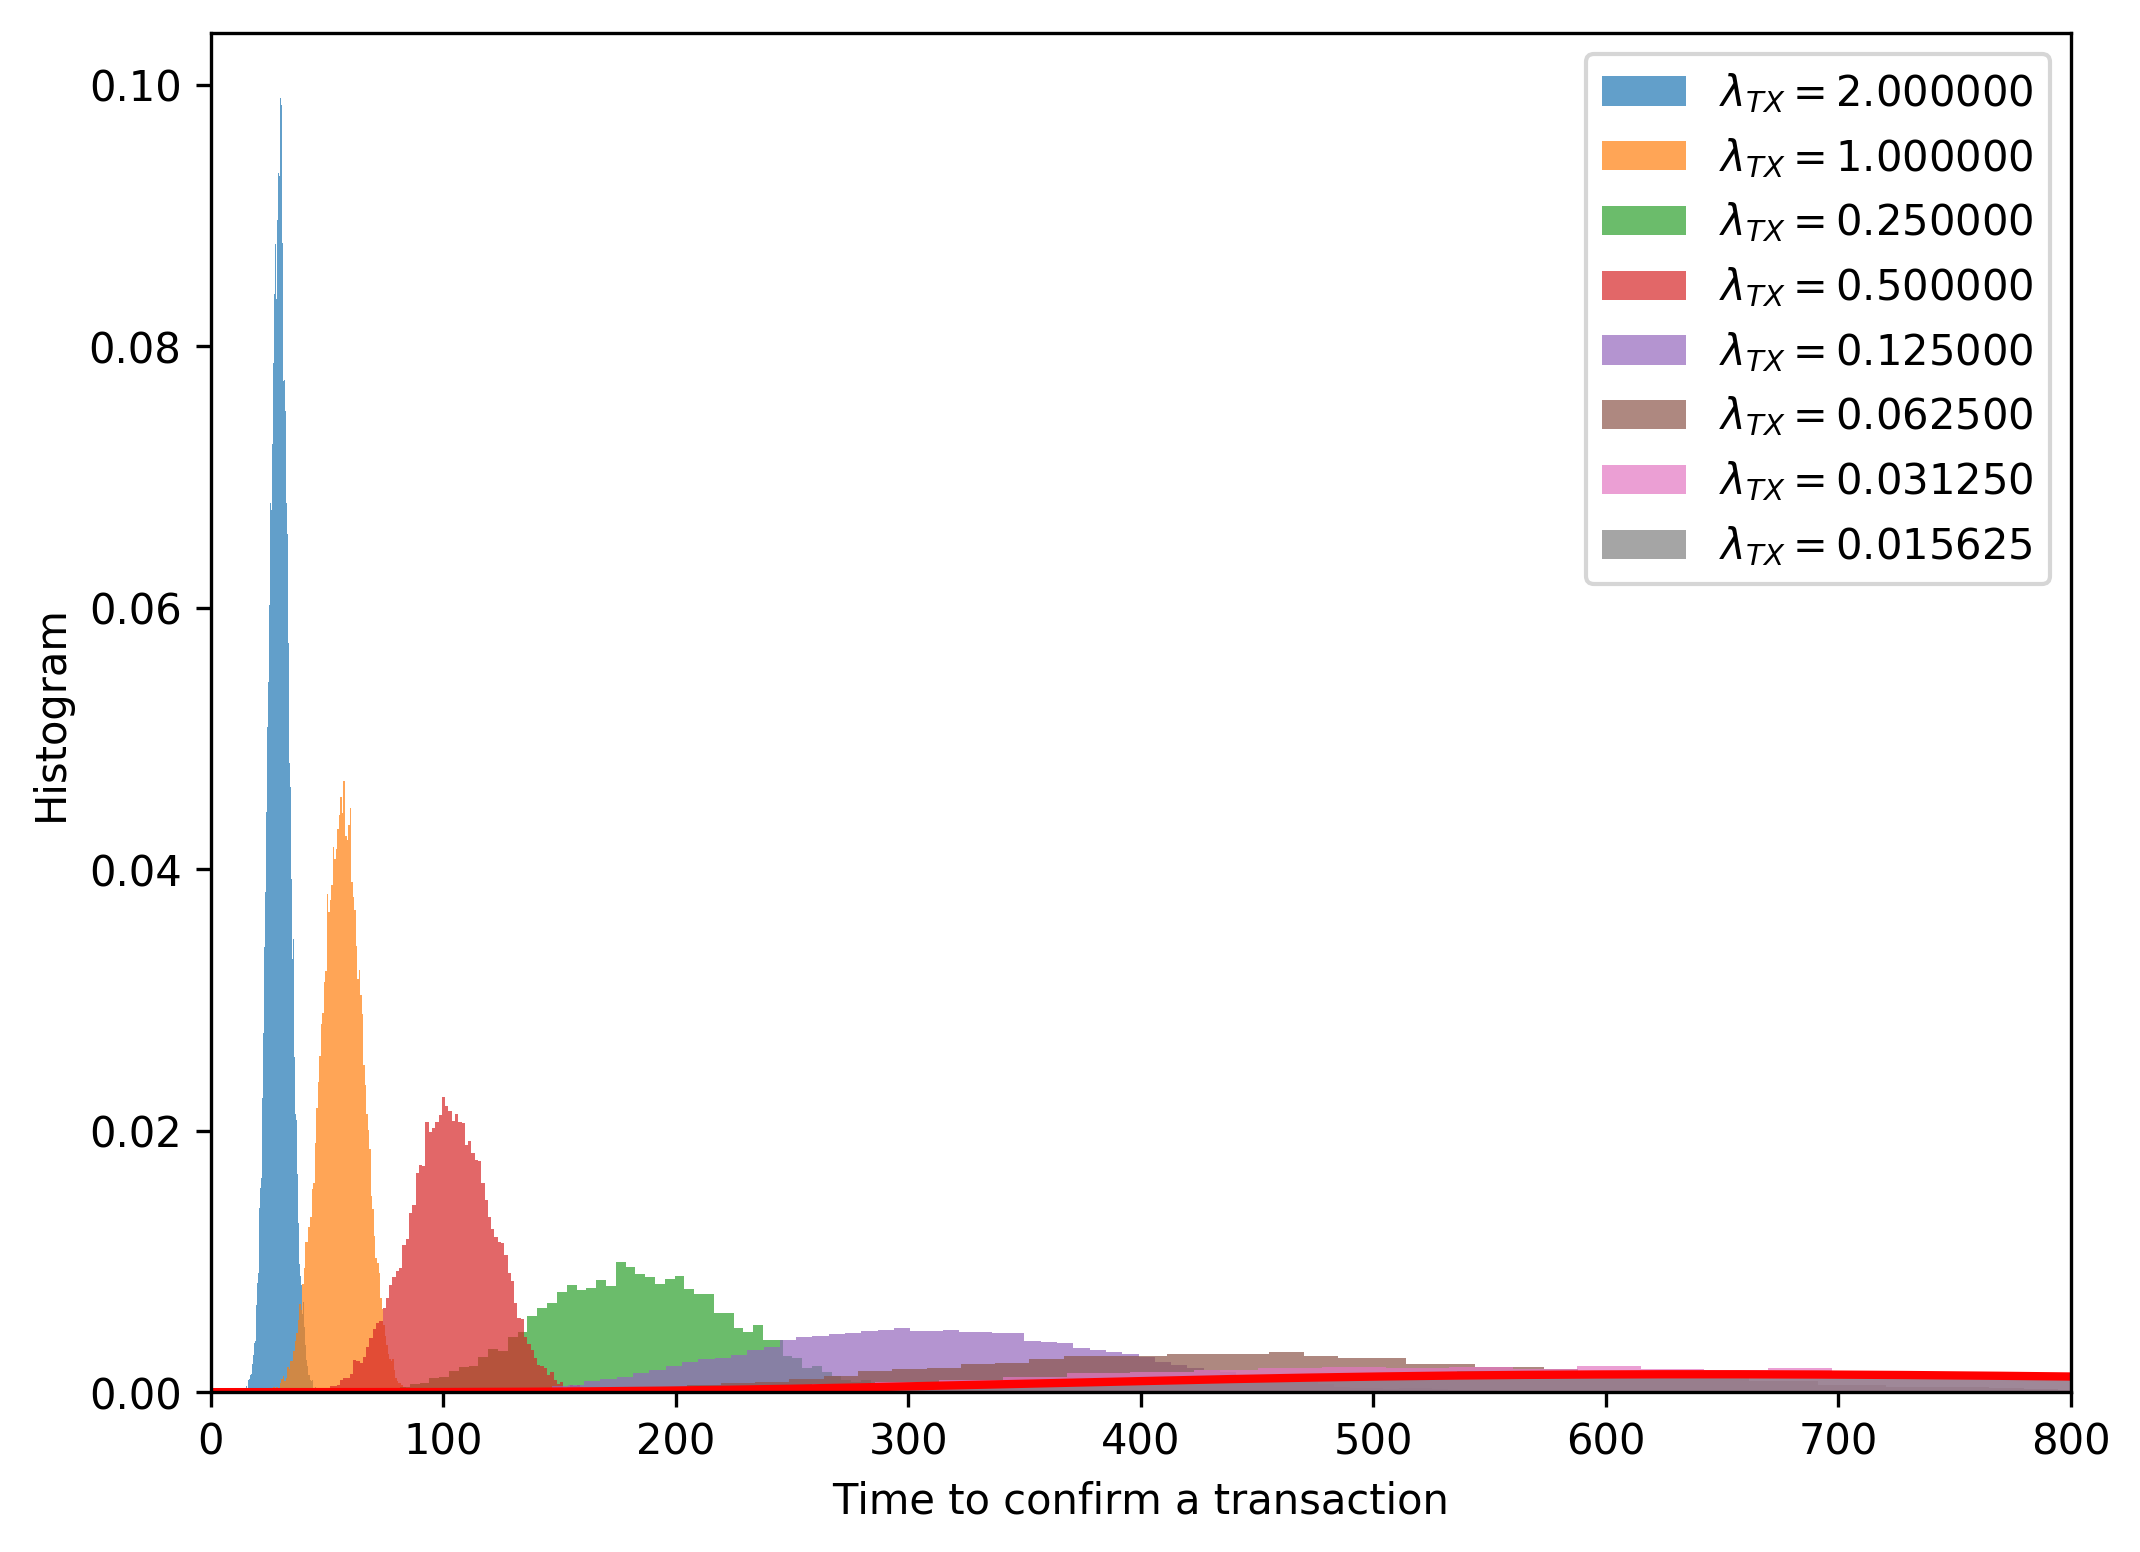
\includegraphics[width=\textwidth]{./images01/sim/tct-many-loads-2.png}}

\subfloat[Zoom in the left part of the above chart]{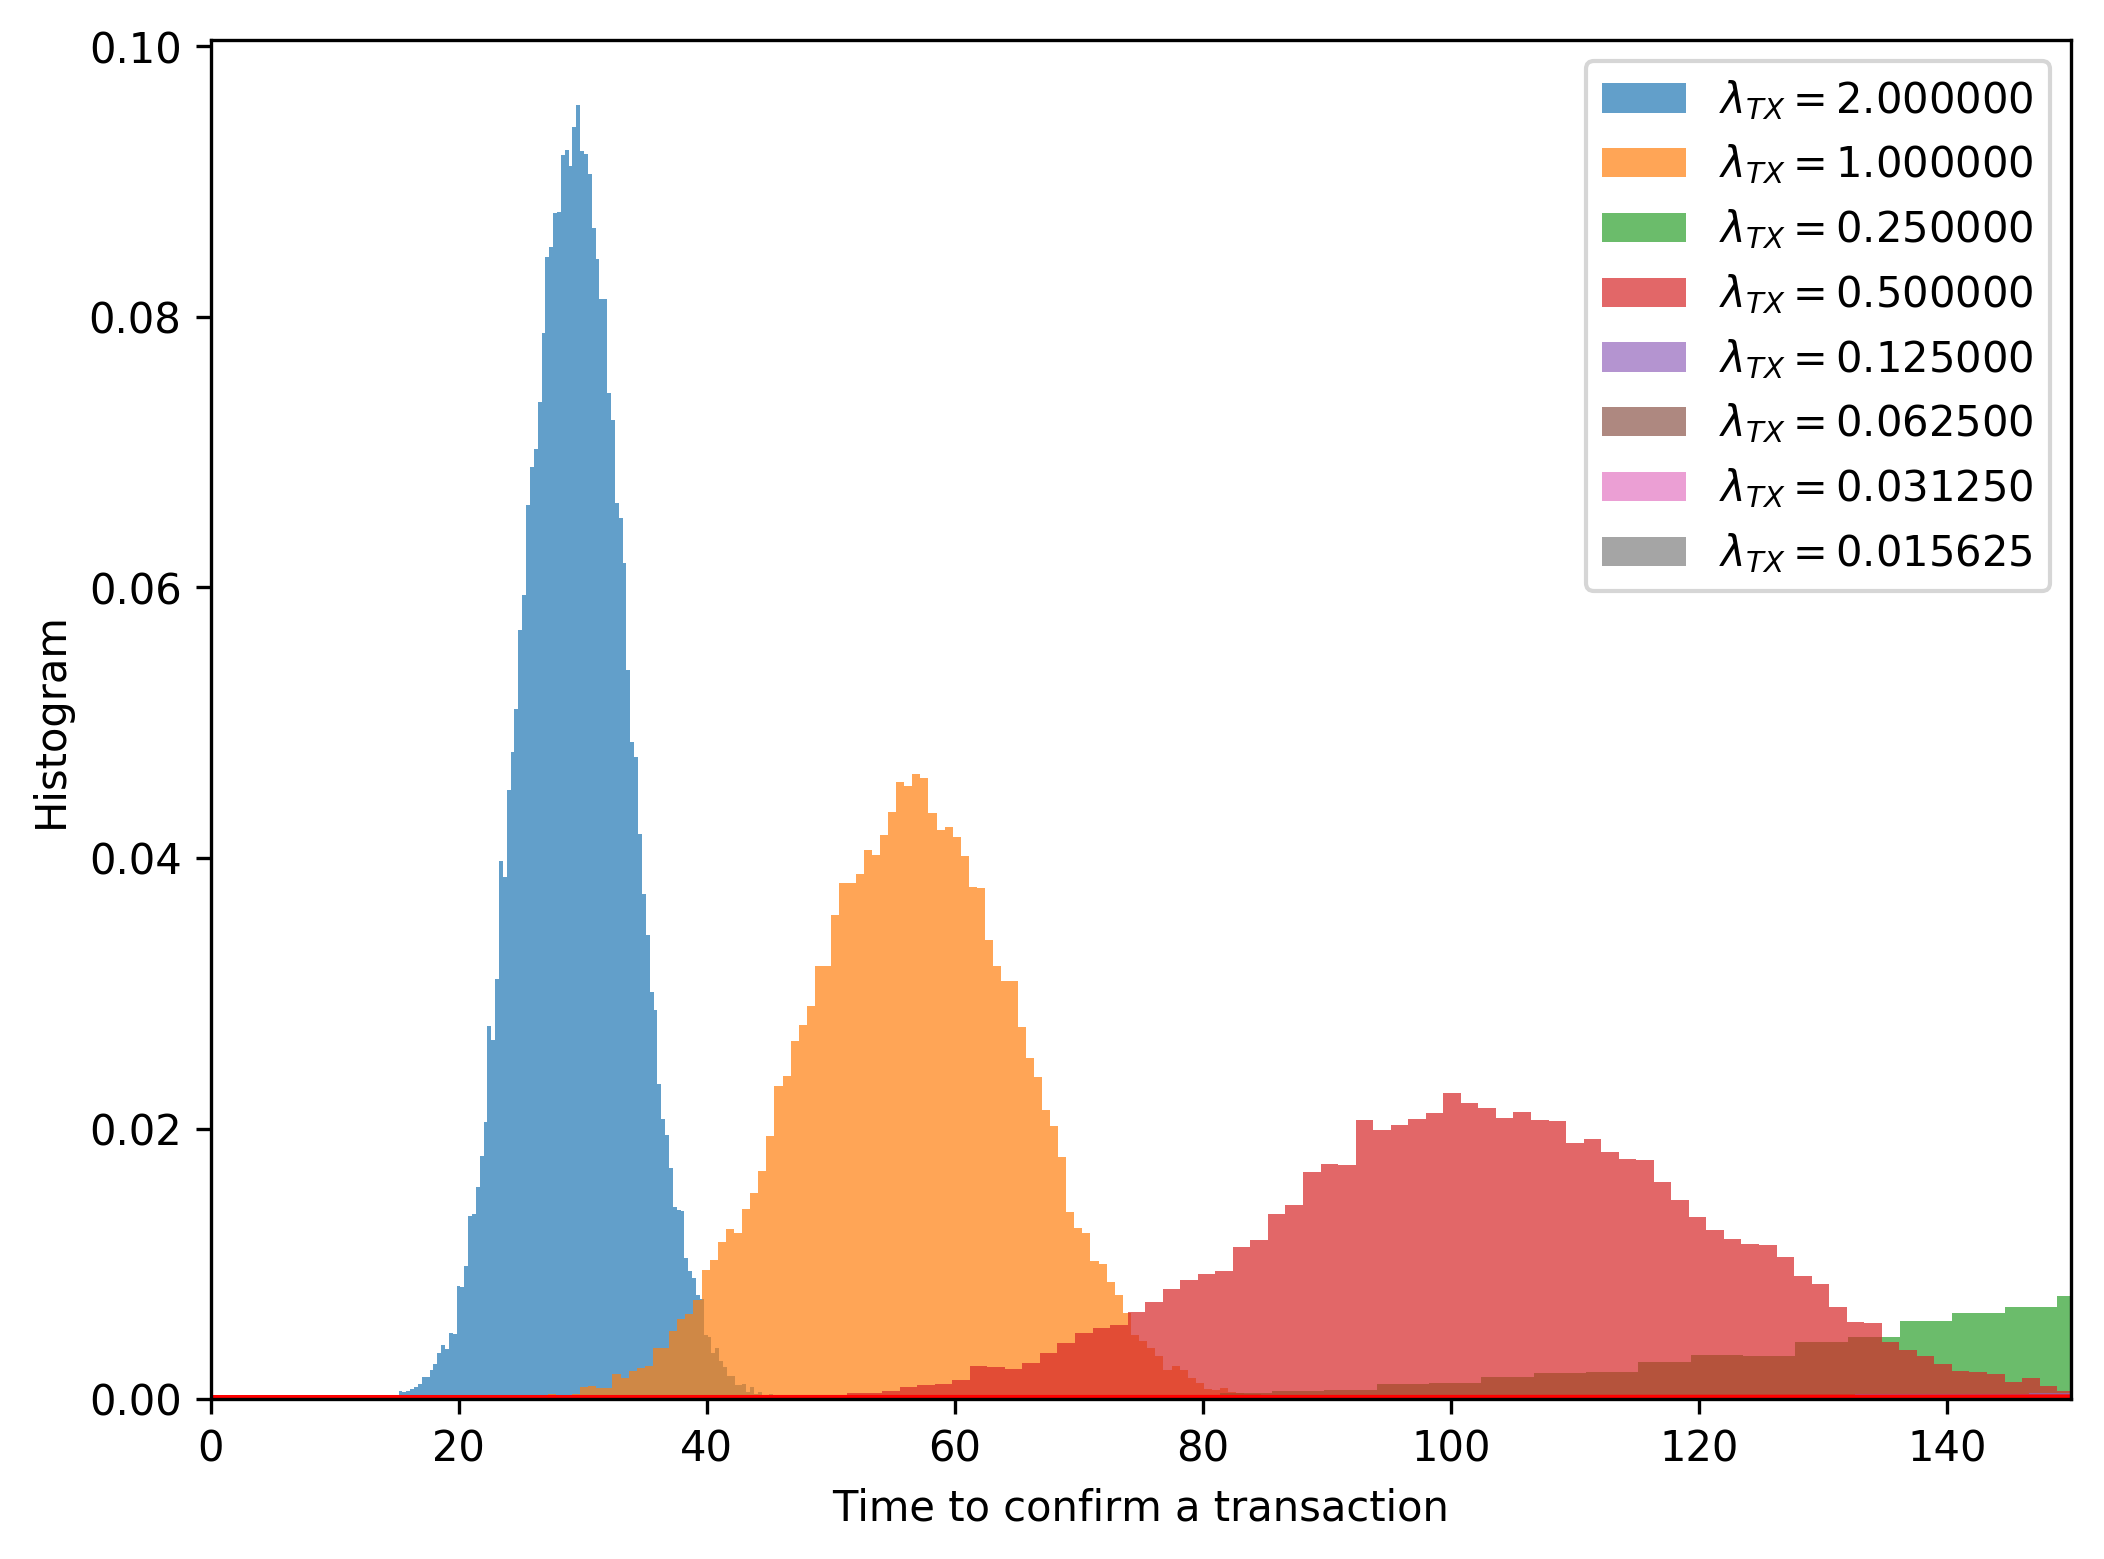
\includegraphics[width=0.5\textwidth]{./images01/sim/tct-many-loads-3.png}}
\subfloat[Zoom in the right part of the above chart \label{fig:hathor-tct-many-right}]{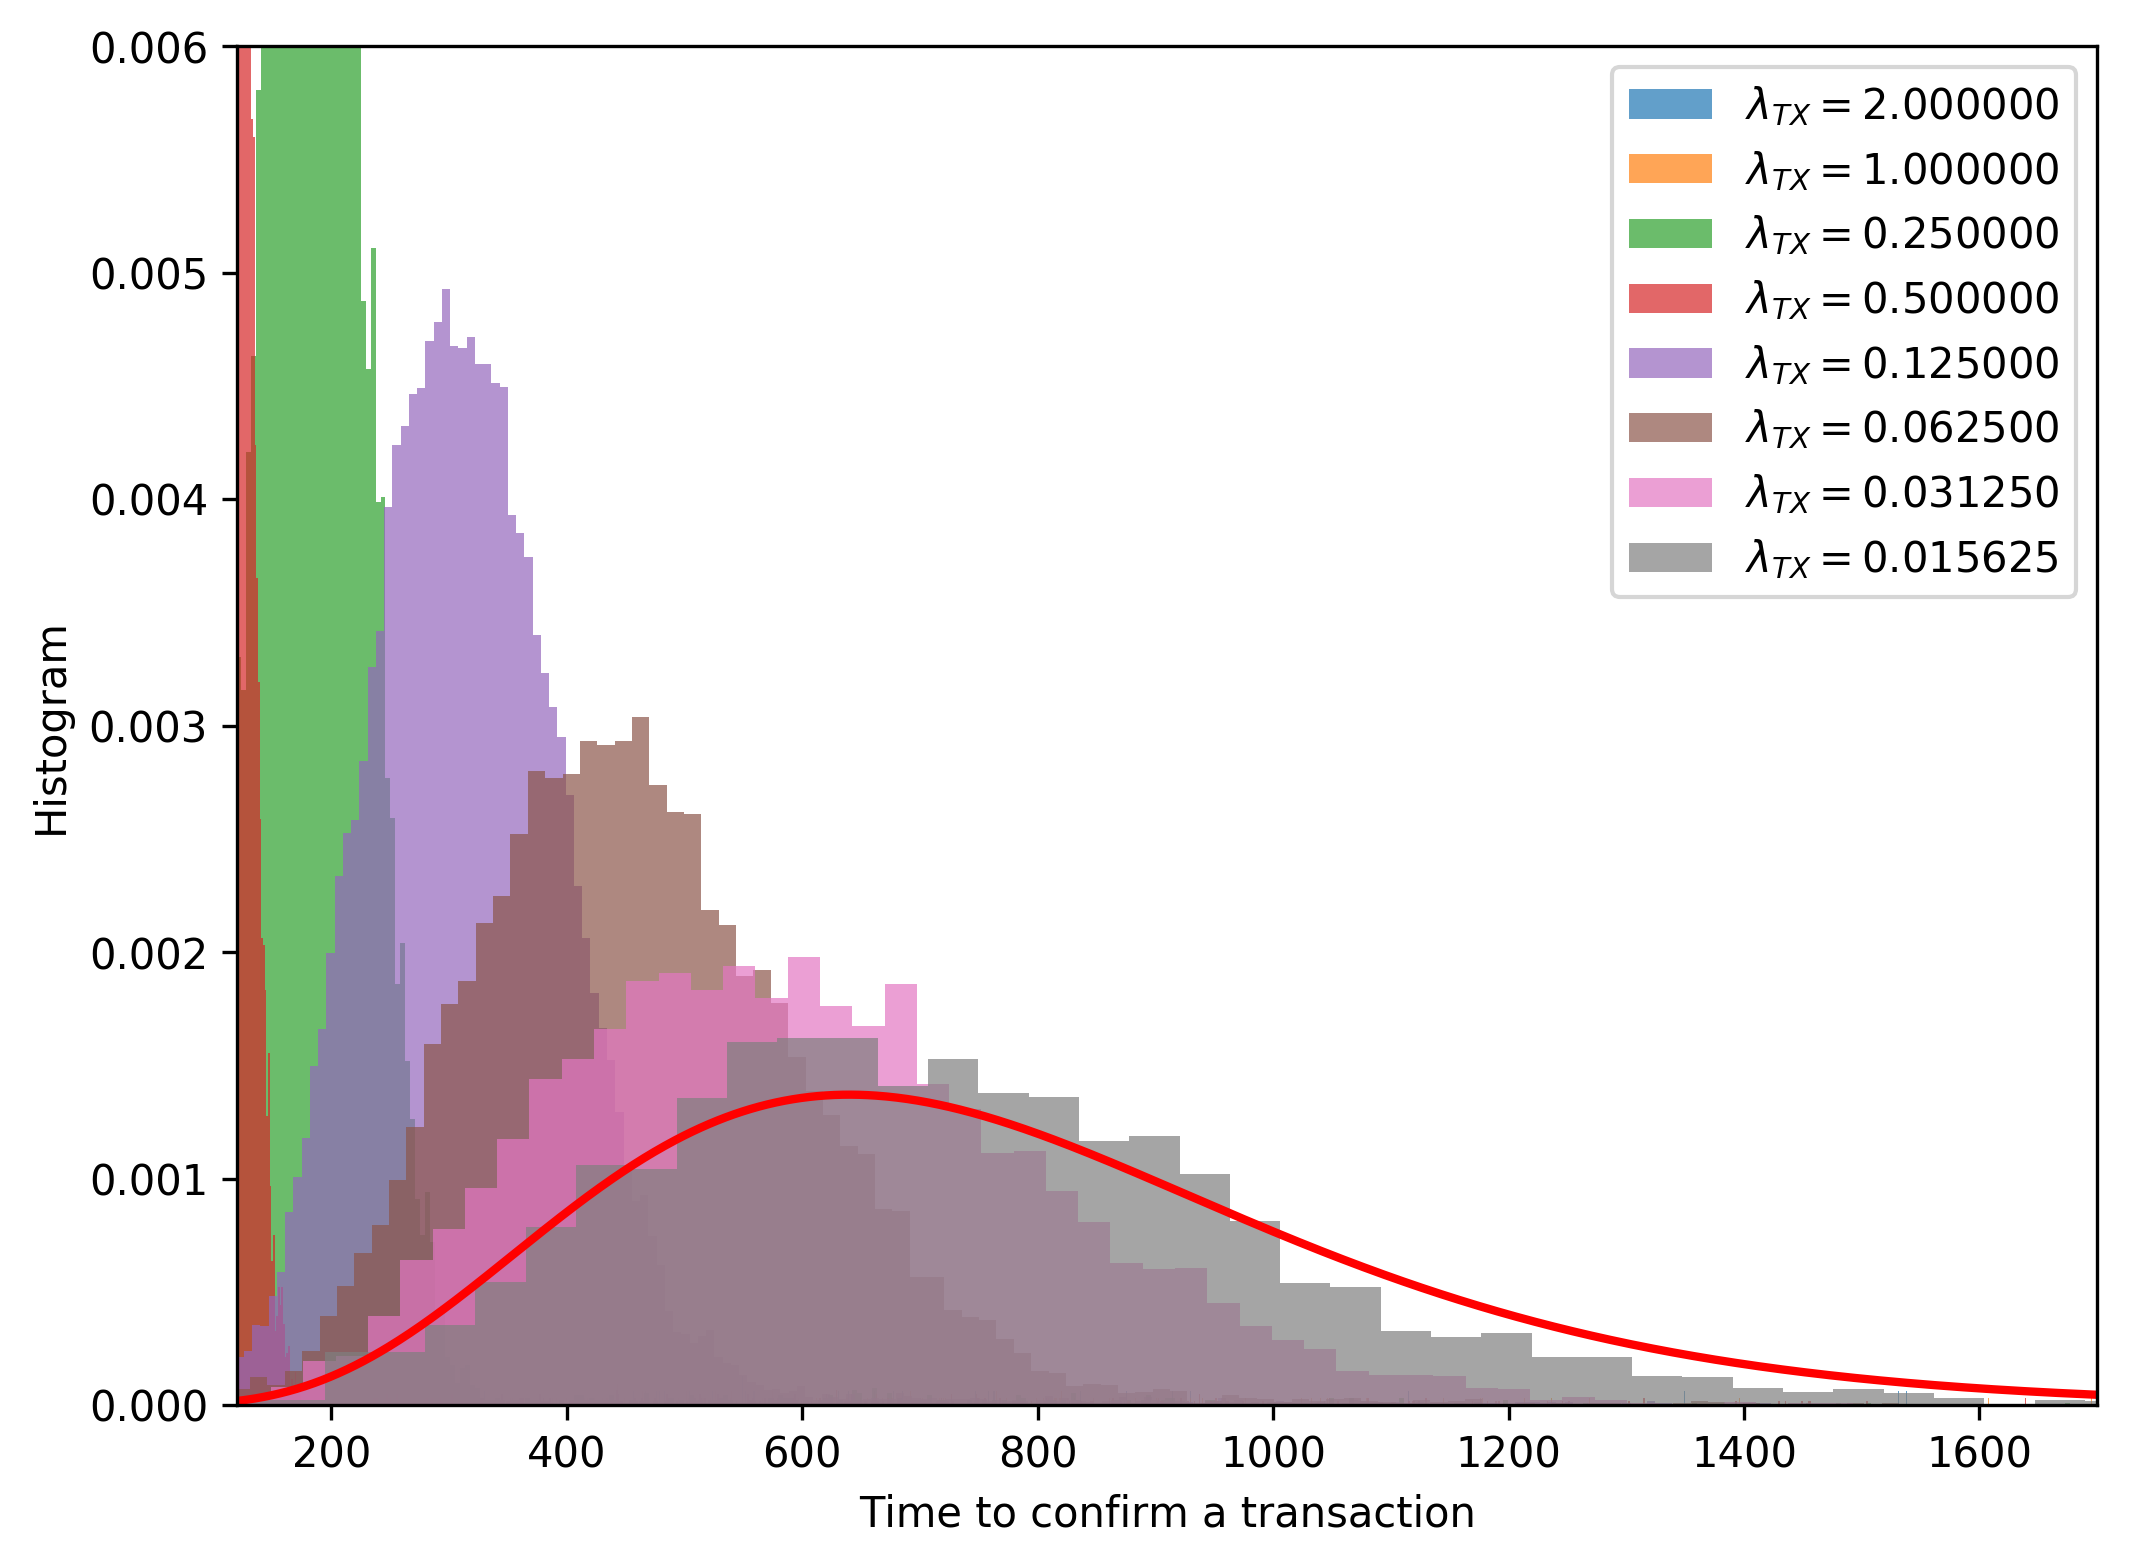
\includegraphics[width=0.5\textwidth]{./images01/sim/tct-many-loads-4.png}}

\caption{Confirmation time in many scenarios, moving from a low load ($\lambda_\text{TX} = 0.015625$) to a high load ($\lambda_\text{TX} = 2$). \label{fig:hathor-tct-many}}
\end{figure}

But, what would happen if, instead of changing the number of transactions per second, we change the relative hash power between miners and transactions? In previous simulations, the miners had a hash rate in the same magnitude as the transactions. In Figure \ref{fig:hathor-tct-100k-10k}, we can see the same simulation as in Figure \ref{fig:hathor-tct-mid-load}, but with the miners' hash rate ten times the transactions'. Besides the difference in the shape of the distribution, we can see that it is moving back towards Bitcoin's confirmation time distribution. It also makes sense because increasing the miners' hash rate increases the required minimum accumulated weighted for confirmed transactions. Therefore, more transactions are necessary to give more accumulated weight. As the number of transactions per second was not changed, most of the work of confirmations were done by blocks (and not by transactions). To confirm this idea, I kept the miners' hash rate ten times the transactions' and increased 16 times the number of transactions per second. As we can see in Figure \ref{fig:hathor-tct-100k-10k-high}, when the number of transactions per second is increased, its role in the accumulated weight also increases and it goes farther from Bitcoin's distribution.

\begin{figure}[!htb]
\centering
\subfloat[Same load as in Figure \ref{fig:hathor-tct-mid-load}]{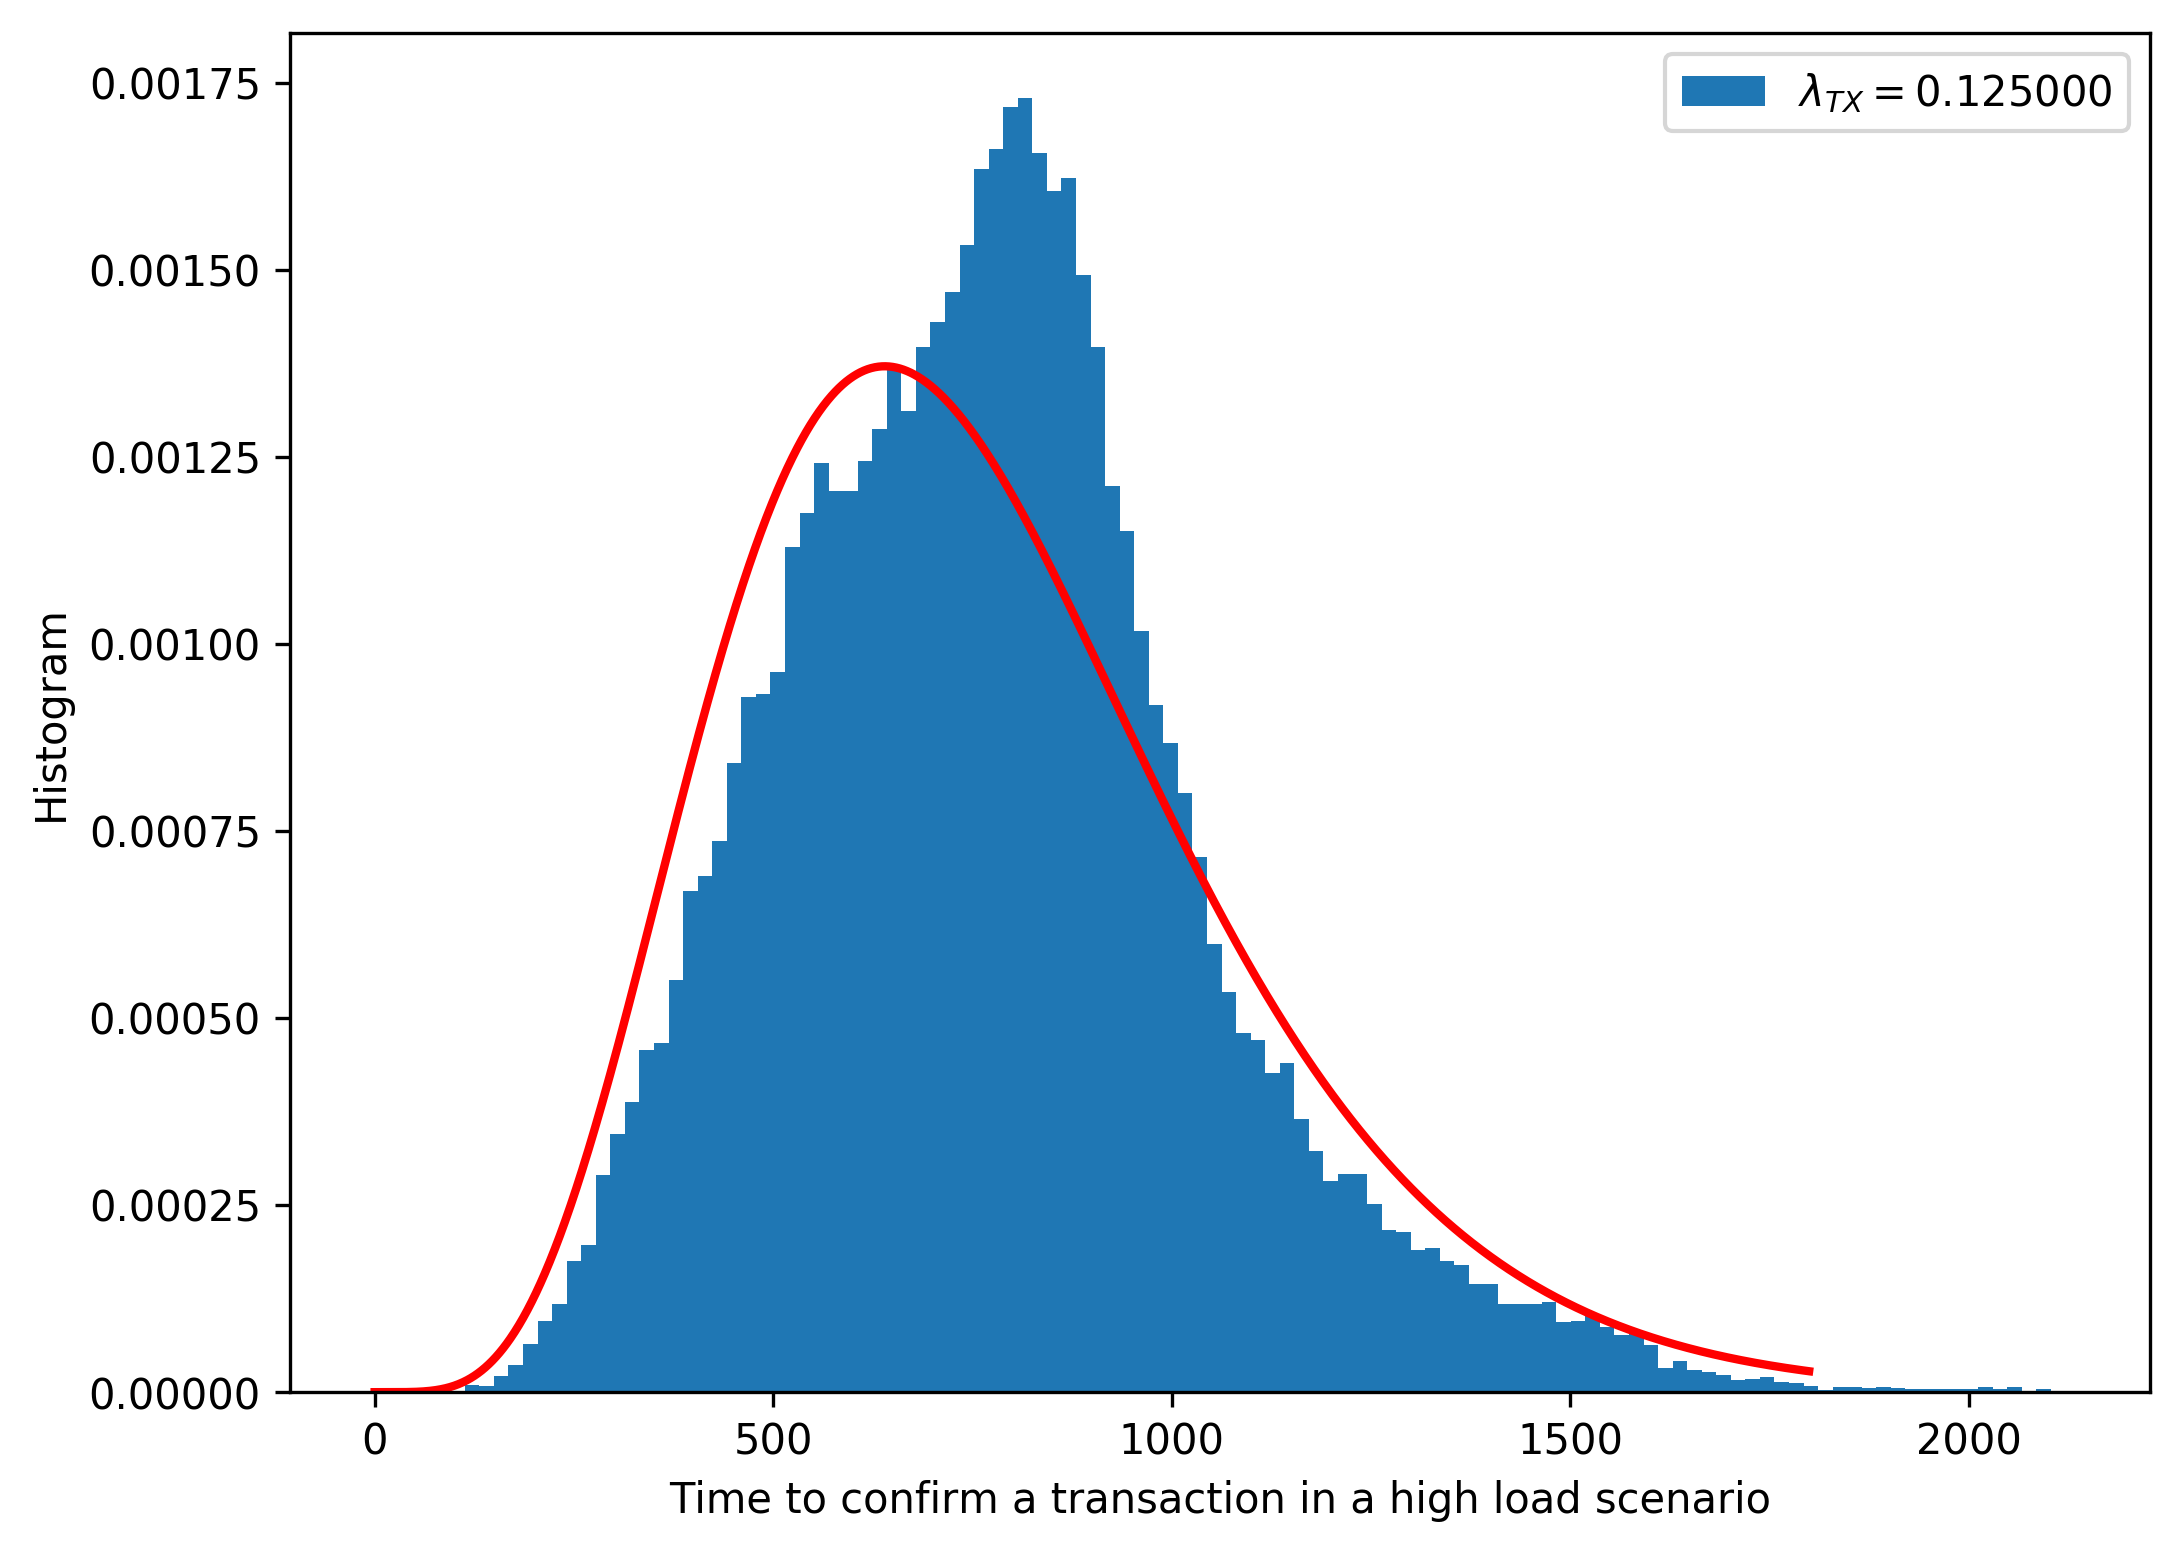
\includegraphics[width=0.5\textwidth]{./images01/sim/tct-100k-10k.png}}
\subfloat[High load, 16 times of (a)\label{fig:hathor-tct-100k-10k-high}]{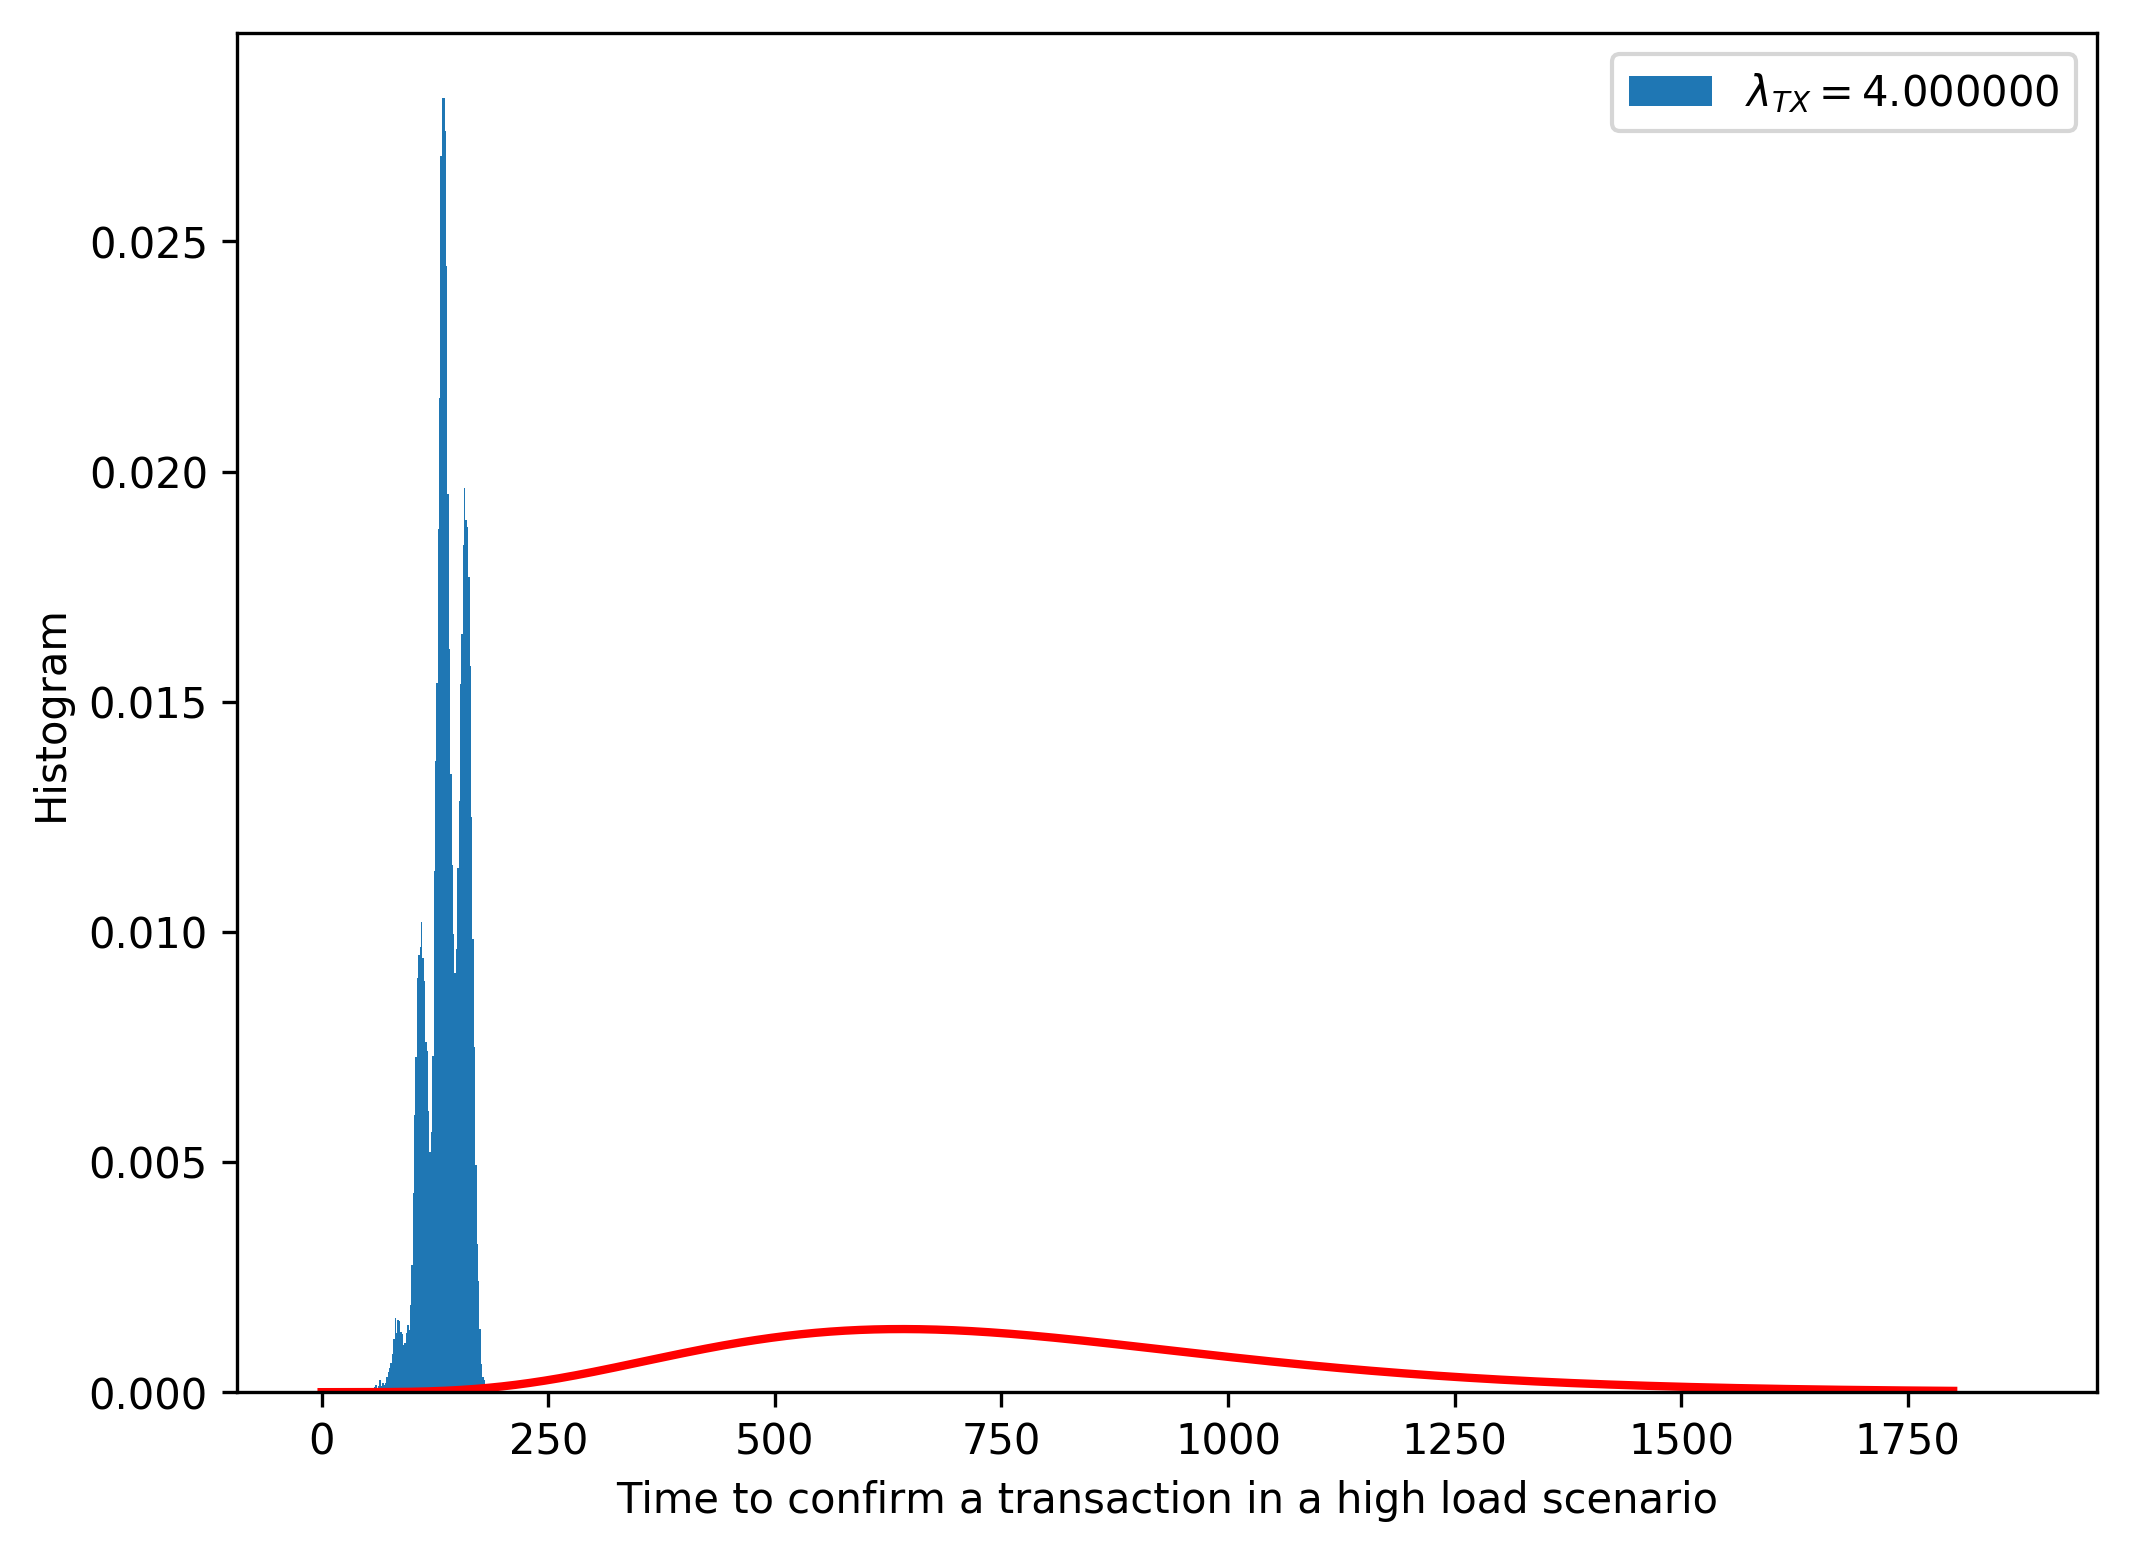
\includegraphics[width=0.5\textwidth]{./images01/sim/tct-100k-10k-high-load.png}}

\caption{Confirmation time with miners' hash rate ten times the transactions'. \label{fig:hathor-tct-100k-10k}}
\end{figure}

Finally, even with both blocks and transactions, Hathor's blocks are similar to Bitcoin's blocks, and they share the same math. To confirm that, see Figure {fig:hathor-tbb}, where the red curve is Bitcoin's distribution of time between blocks and the blue histogram is Hathor's time between blocks. I also made several tests adding and removing miners to check the difficulty adjustment and it worked properly.

\begin{figure}[!htb]
\centering
\subfloat[1 miner]{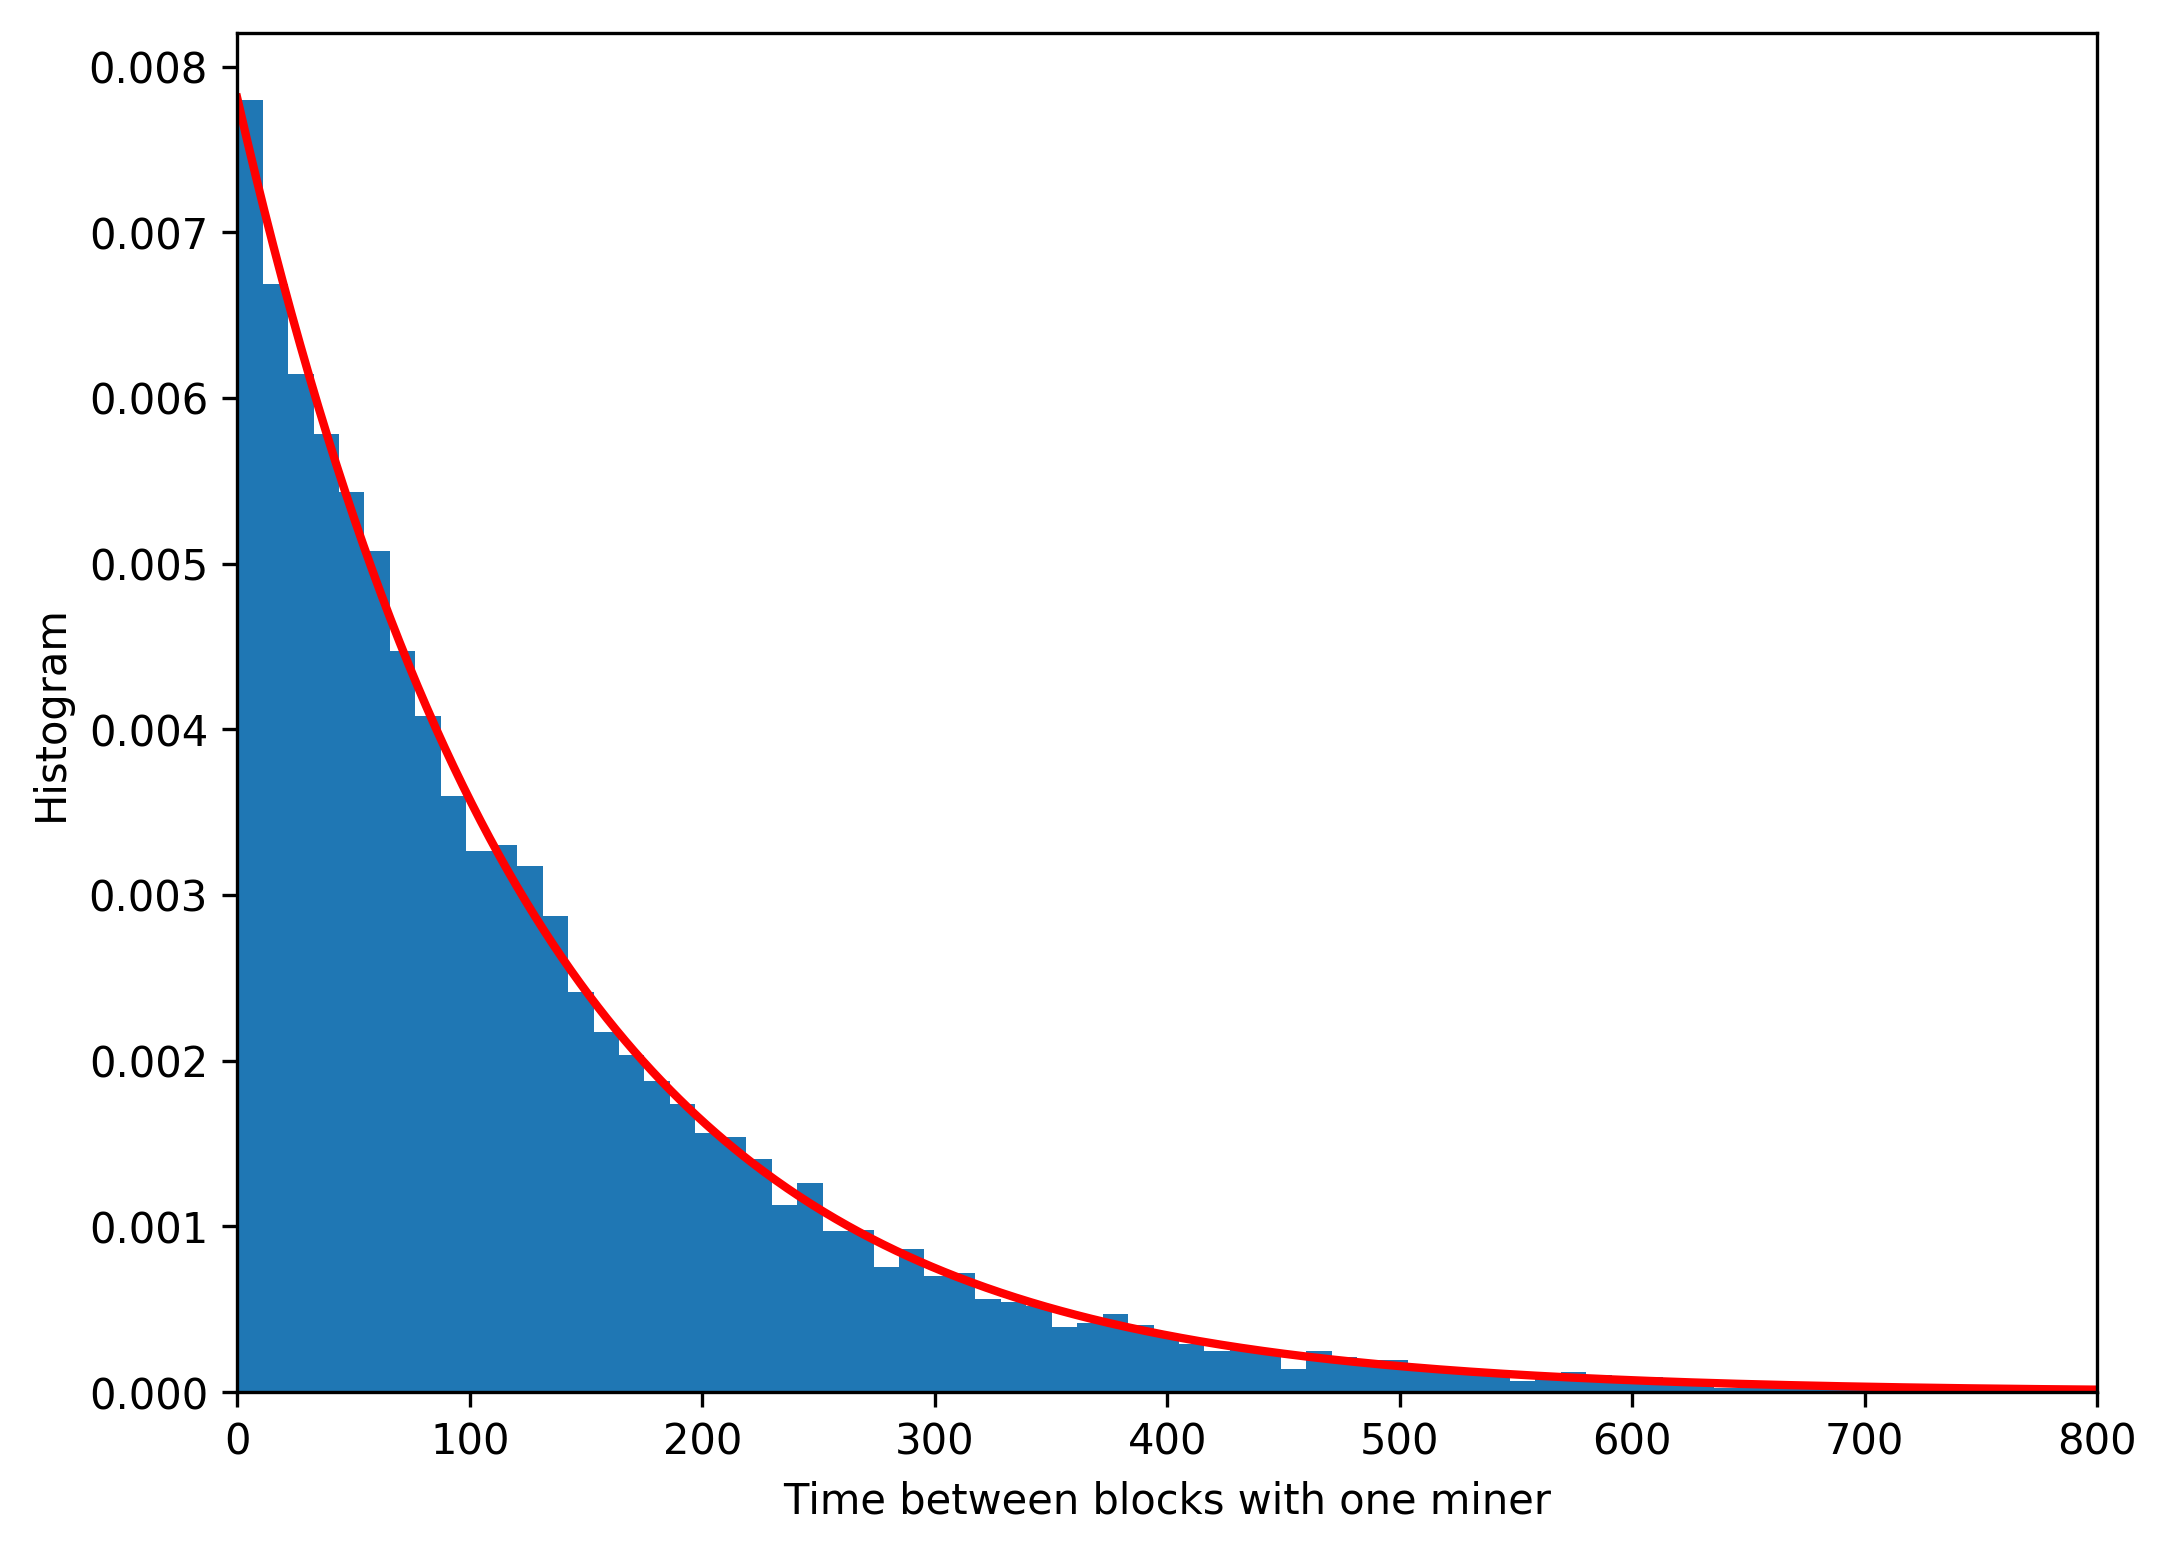
\includegraphics[width=0.5\textwidth]{./images01/sim/tbb-1.png}}
\subfloat[2 miners after difficulty adjustment]{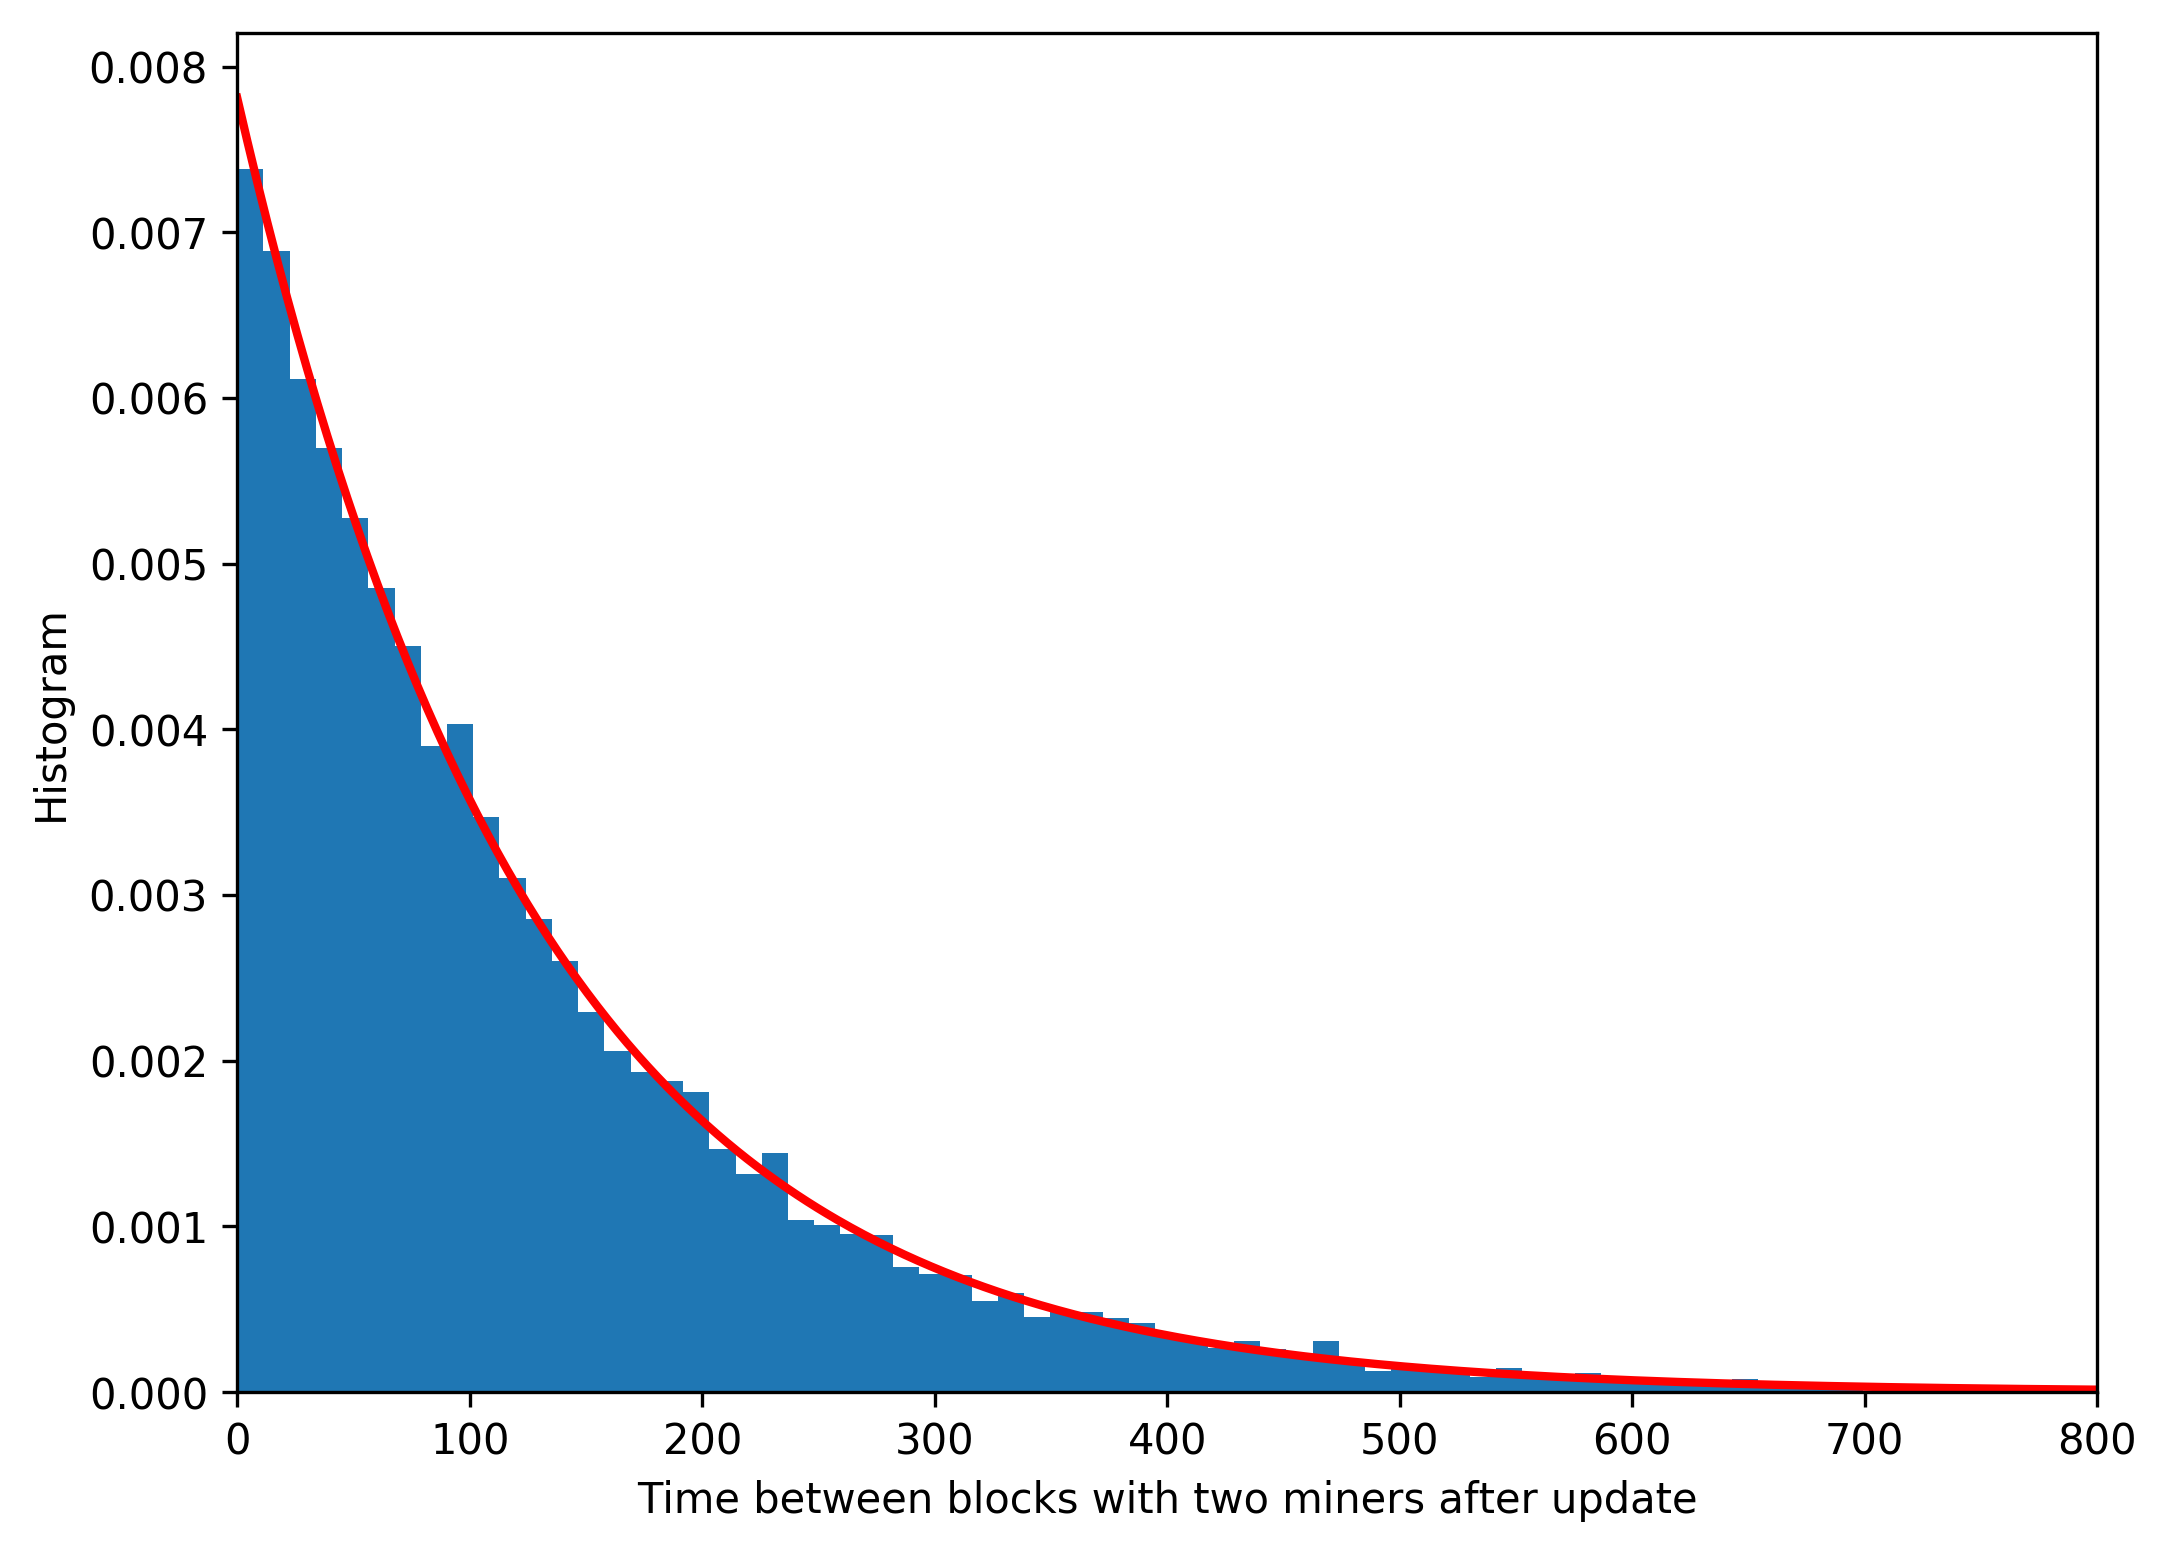
\includegraphics[width=0.5\textwidth]{./images01/sim/tbb-2-after.png}}

\caption{Histogram of time between blocks. The red curve the Bitcoin's theoretical distribution of time between blocks. As we can notice, the fit is very good. \label{fig:hathor-tbb}}
\end{figure}

Afterward, to a better visualization of a Hathor's network, I run a simulation classifying the transactions in either confirmed, in-progress, or unconfirmed (tips). I also showed the transactions solving the proof-of-work which had not been propagated yet. See Figure \ref{fig:hathor-dag-big} and notice the chain of blocks inside the DAG.

\begin{figure}[!htb]
\centering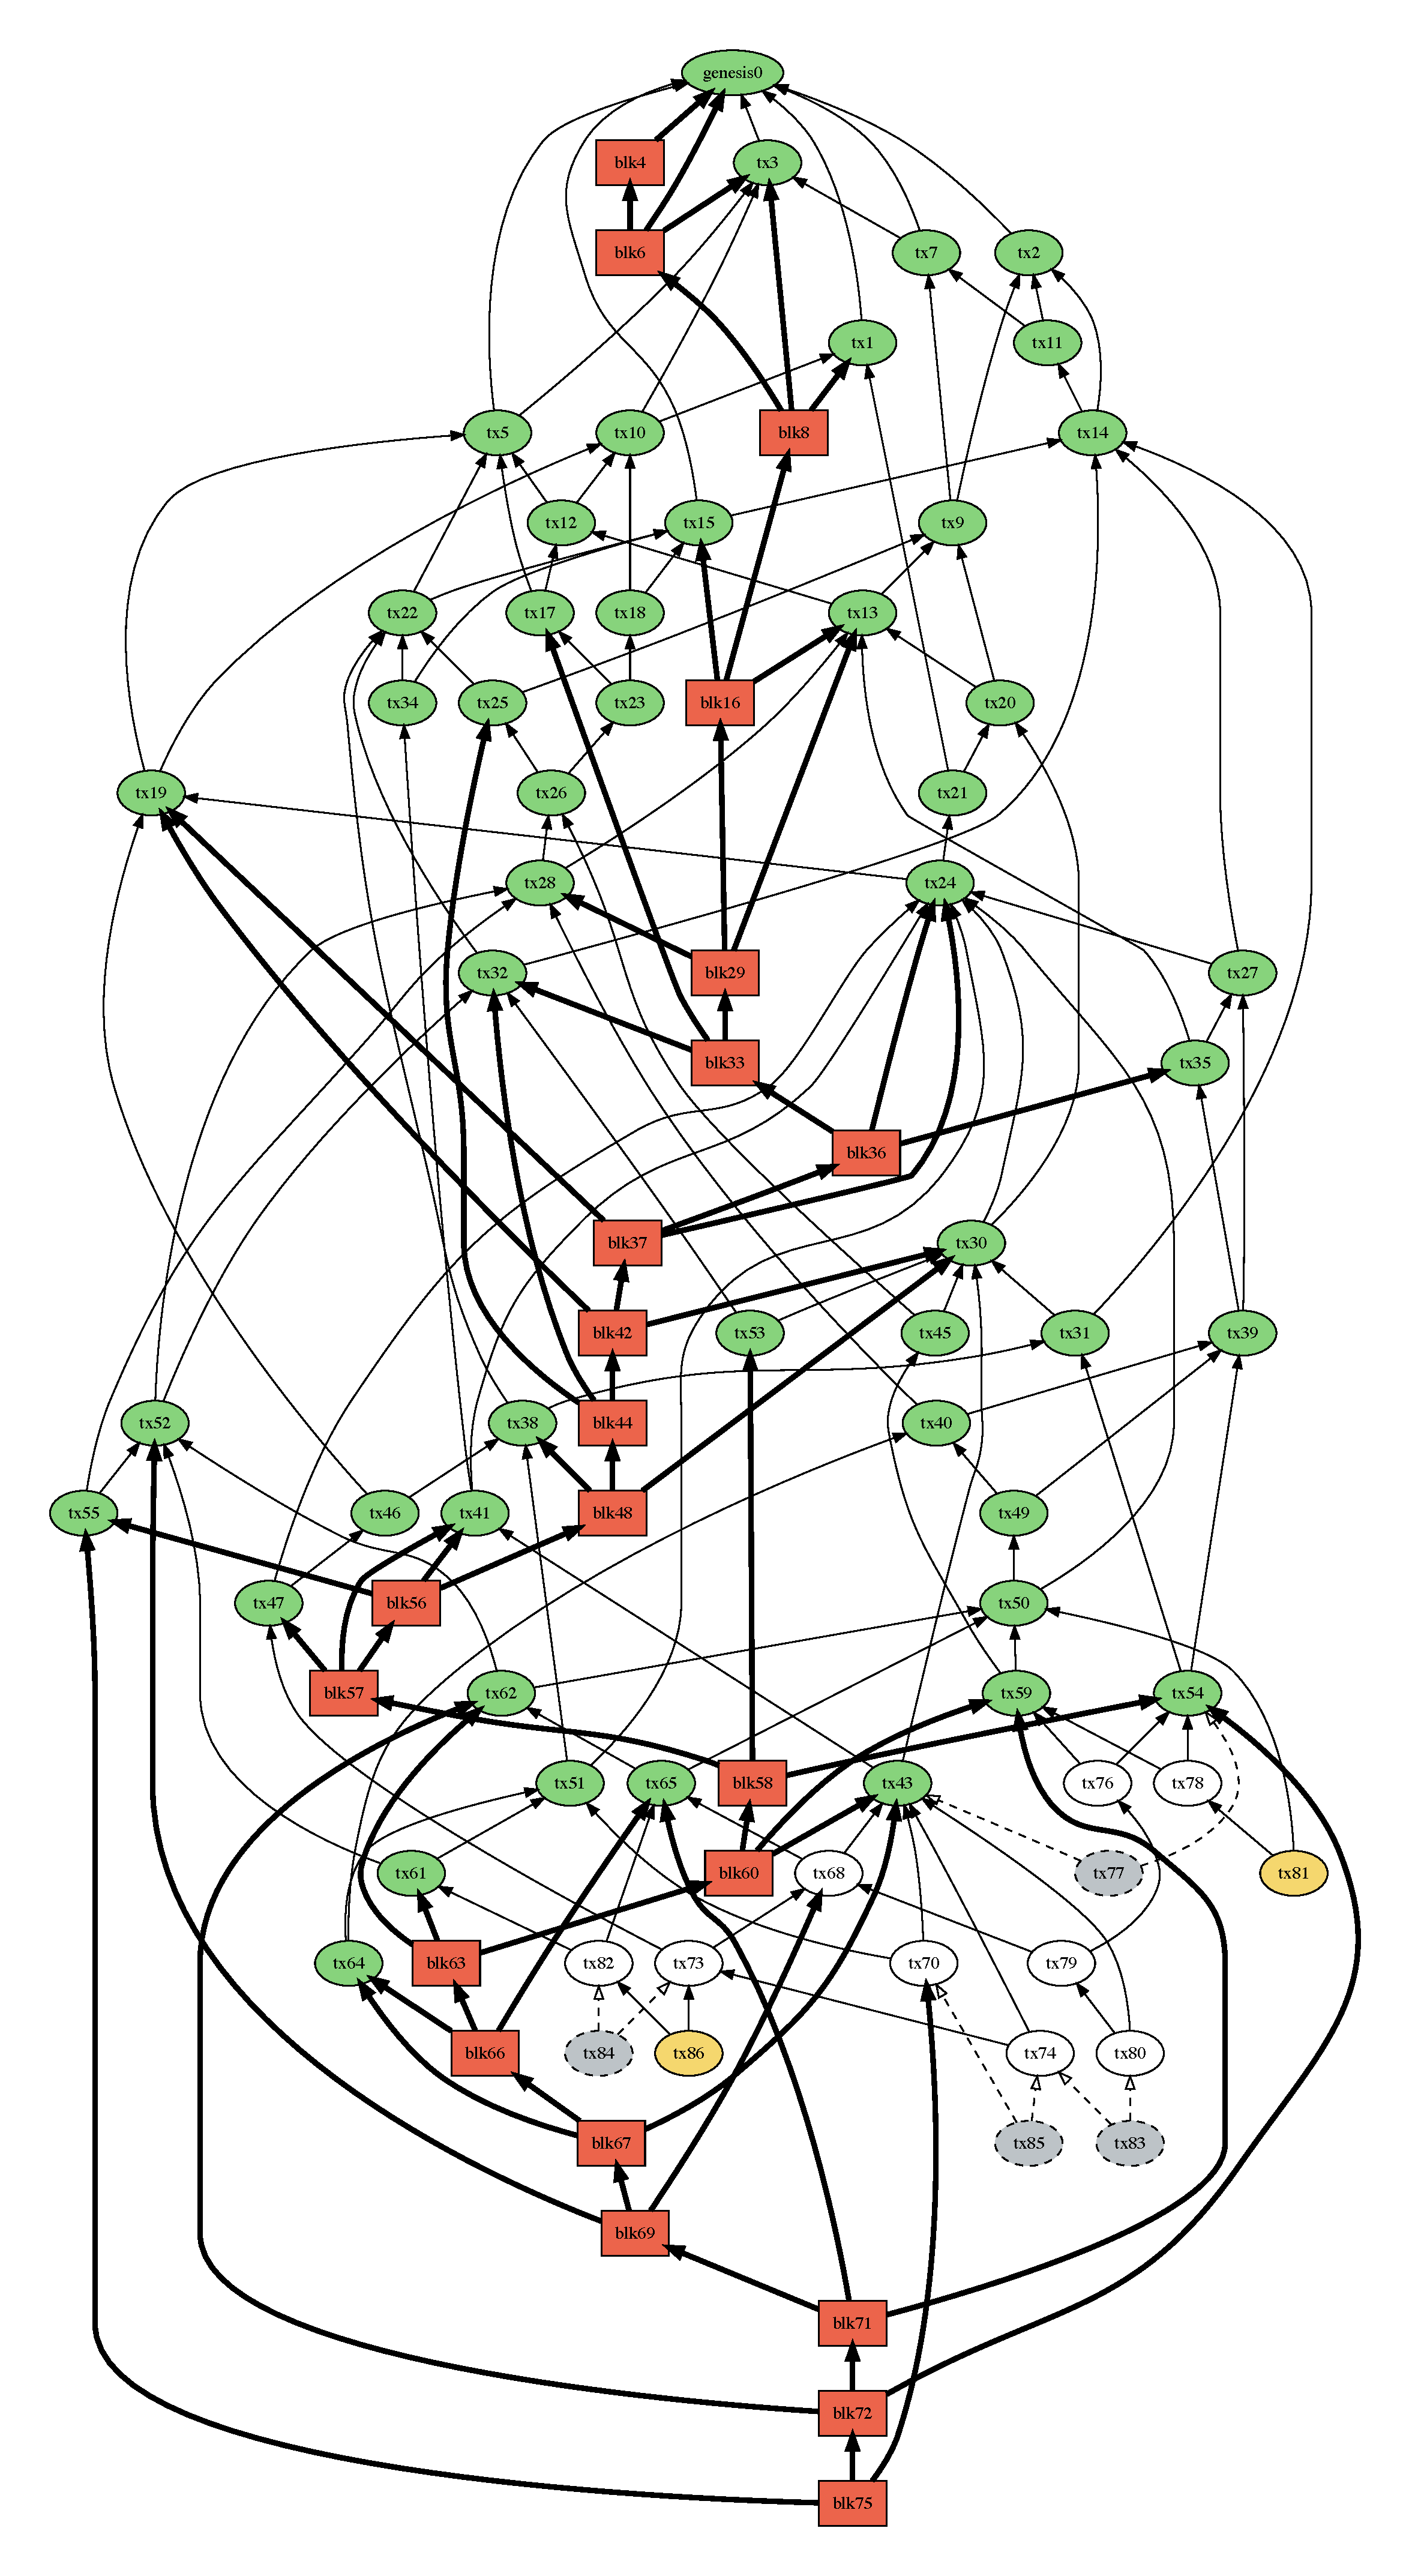
\includegraphics[width=\textwidth]{./images01/sim/hathor-2.pdf}
\caption{Visualization of a Hathor's graph with transactions and blocks. Red boxes are blocks; green circles are confirmed transactions; white circles are in-progress transactions; yellow circles are unconfirmed transactions (tips); and grey circles are transactions solving the proof-of-work which have not been propagated yet. The arrows show the confirmation chain. Block's arrows are in bold. \label{fig:hathor-dag-big}}
\end{figure}

%The number of transactions solving the proof-of-work may be modeled by a Birth and Death process, since if we have $k$ transactions solving the proof-of-work only two things may happen: either a new transaction will be created or one the transactions will finish solving the proof-of-work. Let the time between new transactions follows an exponential distribution with $\mu$ parameter, then the probability of a new transaction emerges before any transaction finishes its proof-of-work is $q_k = \mathbf{P}(T_{\text{new tx}} = \min\{T_{\text{new tx}}, T_1, T_2, \dots, T_k\}) = \frac{\mu}{\mu + \sum_{i=1}^k \lambda_i}$. Hence, the probability of any transaction finishes its proof-of-work before a new transaction emerges is $p_k = 1 - q_k = \frac{\sum_{i=1}^k \lambda_i}{\mu + \sum_{i=1}^k \lambda_i}$.

\begin{theorem}
\label{theorem-new-tx-not-tip}
When a new transaction confirms an already confirmed transaction, the depth of all transactions remains the same, i.e., the depth of the transactions are only changed when a new transaction confirm an unconfirmed transaction.
\end{theorem}

\begin{theorem}
The height of a transaction is equal to the maximum height of its parents plus one.
\end{theorem}

\begin{theorem}
If new transactions choose randomly the unconfirmed transactions to be confirmed, then no unconfirmed transaction will be left behind, i.e., all transactions will be confirmed in due time.
\end{theorem}

\chapter{Conclusion}

Bitcoin's underlying technology blockchain has been called by many as a major invention, even comparable to the invention of the internet. But it is unlikely that Bitcoin and blockchain have achieved the final or most optimal design for a secure and scalable electronic transaction system. In this work, I proposed and analysed a new architecture named Hathor, which seems a scalable alternative to Bitcoin.

Today, Bitcoin network can barely handle 8 transactions per second without increasing the unconfirmed transaction list to hundreds of thousands --- several transactions take days to be confirmed. In order to increase Bitcoin's capacity, its community has first proposed and implemented segregated witness, which was not enough. Finally, they proposed the lightning network, which is in development and should be available in the next months.

- What is better: solves a PoW with $w$, or solves $n$ PoWs with $w/n$?

%\chapter{Proposal: Questions to be explored}

%Given these preliminaries, these are some questions with which we will be concerned.


%In this paper, we will analyze the network scaling and security. How a Hathor network scales, simulating different loads and measuring the bandwidth, computational effort, and storage space necessary to handle all the transactions in time. What is the minimum transaction's aggregated weight which it may be considered unlikely to be reversed?

%We are interested in how the rate of new transactions affects how long it takes to a new transaction to be confirmed for the first time. We had already run some simulations under normal load (Fig. \ref{fig-tangle-hist}) and high load (Fig. \ref{fig-tangle-hist-2}).

%\begin{figure}[ht]
%\centering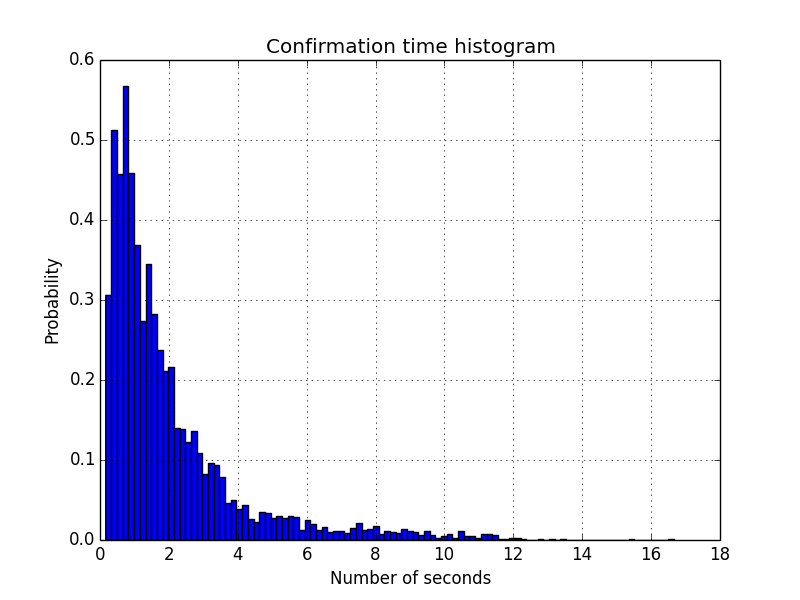
\includegraphics[width=\textwidth]{./images01/fig-tangle-hist.png}
%\caption{Histogram of how long has been a transaction waiting until its first confirmation. It was a simulation of 15 minutes with new transactions rate changing between 1 and 15 tx/s.\label{fig-tangle-hist}}
%\end{figure}

%\begin{figure}[ht]
%\centering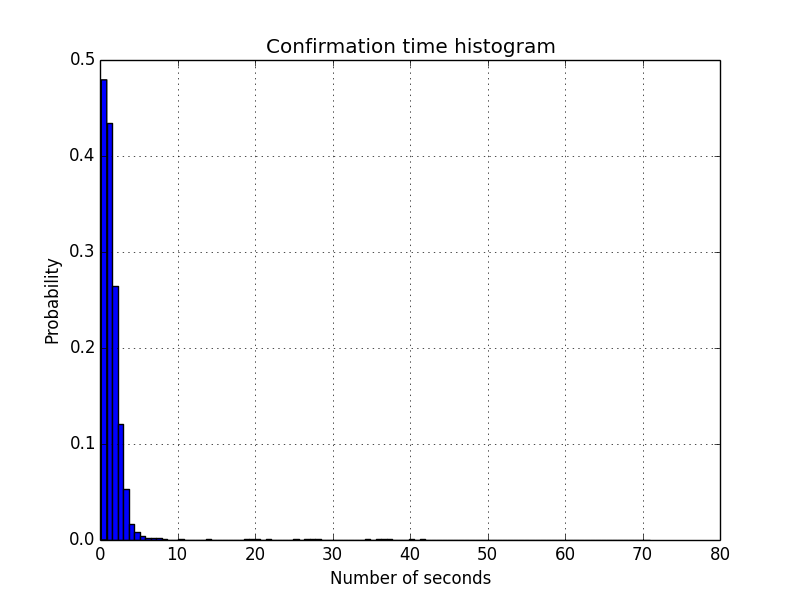
\includegraphics[width=\textwidth]{./images01/fig-tangle-hist-2.png}
%\caption{Histogram of how long has been a transaction waiting until its first confirmation. It was a simulation of 5 minutes with new transactions rate of 50 tx/s, i.e., very high load.\label{fig-tangle-hist-2}}
%\end{figure}


%Besides the time to the first confirmation, it is also important to measure how long it takes to a new transaction reach a specific accumulated weight. It is useful for exchanges and merchants to set their minimum requirements. Bitcoin's exchanges and merchants usually requires a minimum of 6 confirmations blocks.

%OLD \cite{tangle2016} suggests that constraining transactions' weight in a range would both prevent spam, because it would be necessary a minimum work to propagate a new transaction, and attacks, because an attacker would not be allowed to propagate a transaction with very high weight. We agree with the spam argument, and would like how a minimum weight would affect mobile devices's new transactions. We partially agree with the upper bound, because an attacker would be able to generate many transaction with lower weight. We will analyze if constraining transactions' weight would be effective against nuclear submarine attacks.

%OLD We have another suggestion to prevent nuclear submarine attacks: set a maximum depth for the transactions confirmed by a new transaction. So, new transactions would have to confirming newer transactions instead of old transactions, and a nuclear submarine attack would be controlled because the attacker would be not be able to create a large separate DAG. But the maximum depth rule would possibly also affect transaction created by low (hash)power devices, because it would take a longer time to solve the proof-of-work and, if the confirmations are going fast, the transaction would possibly be invalidated. This raises another important question: what would be an optimal maximum depth allowed?

%OLD If we would like to include fee transactions, how would it be distributed between confirmations? As transactions may have multiple direct confirmations, it is not obvious who would receive the transaction fee. An intuitive suggestion would be to give the fee to the first confirmation with a minimum weight, but it might have some propagation problems, because it takes a while to propagate a transaction in the network and there would be conflict.

%OLD In order to solve the fee distribution problem, we will simulate how the network would behave if we include blocks. These blocks would be like Bitcoin's, with an adjustable proof-of-work according to the network's hashpower. They would receive the fees from all confirmed transactions which had not been confirmed by any block before, and they would be able to generate new coins. These blocks would also help solving other problems.

%\begin{enumerate}
%\item Which parameters turns the network more or less vulnerable to attacks?
%\item Is there an optimal strategy to attack?
%\item Could new coins be generated demanding a proof-of-work with dynamic difficulty, like in Bitcoin?
%\item What is the equation of number of tips over time? What is the equation of how long it takes to a transaction to be confirmed for the first time? What is the equation of the accumulated weight of a transaction over time? Some equations have already been proposed by \citet{tangle2016}.
%\end{enumerate}
